% arara: pdflatex
% arara: pdflatex
% arara: pdflatex

% options:
% thesis=B bachelor's thesis
% thesis=M master's thesis
% czech thesis in Czech language
% slovak thesis in Slovak language
% english thesis in English language
% hidelinks remove colour boxes around hyperlinks

\documentclass[thesis=M,czech]{FITthesis}[2019/12/23]

\usepackage[utf8]{inputenc} % LaTeX source encoded as UTF-8

% \usepackage{amsmath} %advanced maths
% \usepackage{amssymb} %additional math symbols

\usepackage{dirtree} %directory tree visualisation

% % list of acronyms
% \usepackage[acronym,nonumberlist,toc,numberedsection=autolabel]{glossaries}
% \iflanguage{czech}{\renewcommand*{\acronymname}{Seznam pou{\v z}it{\' y}ch zkratek}}{}
% \makeglossaries

\newcommand{\tg}{\mathop{\mathrm{tg}}} %cesky tangens
\newcommand{\cotg}{\mathop{\mathrm{cotg}}} %cesky cotangens

% % % % % % % % % % % % % % % % % % % % % % % % % % % % % % 
% ODTUD DAL VSE ZMENTE
% % % % % % % % % % % % % % % % % % % % % % % % % % % % % % 
% https://www.citace.com/CSN-ISO-690.pdf
\usepackage{tabularx}
\usepackage{listings}
\usepackage{tabto}
\usepackage{changepage}
\usepackage{subcaption}
\newenvironment{example}{\begin{adjustwidth}{1cm}{}}{\end{adjustwidth}}
% \titlespacing*{\subsubsection*}{0pt}{3.25ex plus 1ex minus .2ex}{0.5em}

\department{Katedra aplikované matematiky}
\title{Open-source doporučovací systém pro české veřejné zakázky}
\authorGN{Milan} %(křestní) jméno (jména) autora
\authorFN{Vancl} %příjmení autora
\authorWithDegrees{Bc. Milan Vancl} %jméno autora včetně současných akademických titulů
\author{Milan Vancl} %jméno autora bez akademických titulů
\supervisor{Ing. Jaroslav Kuchař, Ph.D.}
\acknowledgements{Především bych chtěl vyjádřit svůj vděk své rodině, která mě podporovala po celou dobu mého studia od začátku až do konce. Děkuji panu Ing. Jaroslavu Kuchařovi, Ph.D. za vřelou komunikaci při odborném i formálním vedení této práce. Dále děkuji panu Ing. Marku Sušickému za oponenturu a záštitu téma a společnosti Profinit EU, s.r.o. za materiální podporu pro účely této práce. V neposlední řadě děkuji slečně Ing. Lucii Svitákové, panu Ing. Davidu Šenkýřovi a panu Mgr. Martinu Popelovi, Ph.D. za poskytnuté konzultace a panu Michalu Bláhovi děkuji za poskytnutí datasetu.}
\abstractCS{
    V této práci se zabývám návrhem a implementací open-source doporučovacího systému pro české veřejné zakázky. Provádím průzkum a hodnocení současných systémů týkajících se veřejných zakázek. Pro doporučovací algoritmus vybírám vlastnosti zakázek, pro které navrhuji a implementuji jejich získávání či extrakci. Za hlavní vlastnost určuji předmět plnění zakázek, ze kterého extrahuji sémantickou informaci pomocí embeddingu. Doporučovací algoritmus demonstruji v jednoduché webové aplikaci.
}
\abstractEN{
    In this thesis I deal with the design and implementation of an open-source recommender system for Czech public procurement. I conduct research and discussion of current systems related to public procurrement. For the recommendation algorithm, I select a set of procurement features for which I design and implement their retrieval and extraction. I determine the main feature as the subject of procurement from which I extract semantic information using embedding. I demonstrate the recomender algorithm with a simple web application.
}
\placeForDeclarationOfAuthenticity{V~Praze}
\declarationOfAuthenticityOption{4} %volba Prohlášení (číslo 1-6)
\keywordsCS{české veřejné zakázky, doporučovací systém, zpracování textu, podobnost textu, text embedding, open-source}
\keywordsEN{Czech public procurement, recommender system, text processing, text similarity, text embedding, open-source}
% \website{http://site.example/thesis} %volitelná URL práce, objeví se v tiráži - úplně odstraňte, nemáte-li URL práce

\begin{document}

% \newacronym{CVUT}{{\v C}VUT}{{\v C}esk{\' e} vysok{\' e} u{\v c}en{\' i} technick{\' e} v Praze}
% \newacronym{FIT}{FIT}{Fakulta informa{\v c}n{\' i}ch technologi{\' i}}

\begin{introduction}
    Veřejné zakázky (dále VZ) jsou nepostradatelnou součástí české státní veřejné správy. Podíl trhu veřejných zakázek na HDP České republiky dosáhl za rok 2018 11,76 \% \cite{mmr2018}, což odpovídá počtu přes 61 tisíc nových zakázek v hodnotě  více než 370 miliard korun\cite{ceskezakazky}. Meziročně potom v České republice přibývá průměrně více než 50 tisíc nových zakázek za stovky miliard korun.
    
    Z hlediska korupčního rizika patří veřejné zakázky k nejvíce ohroženým oblastem veřejného financování. Riziko korupce narůstá kvůli objemu transakcí a finančním  zájmům  zainteresovaných  stran,  ale  také  díky  složitosti  procesu,  úzké  spolupráci  mezi státní  a  soukromou  sférou  a  množství  subjektů,  které  se  zadávání  veřejných  zakázek  účastní\cite{transparency2019}.
    
    Veliký dopad na efektivitu a transparentnost řízení zakázek má elektronizace procesu zadávání, která je v dnešní době již ze zákona povinná. K~tomu slouží hned několik systémů, které se navzájem doplňují nebo si konkurují.
    
    Počet a struktura těchto systémů může být pro nezasvěceného uživatele poněkud nepřehledná. 
    Použití stávajících systémů k vyhledávání zakázek navíc od uživatele z pravidla vyžaduje pokročilý přehled o členění a možných parametrech zakázek, což může znamenat bariéru k dosažení hodnotných informací.
    
    Ovšem i v případě, kdy má uživatel detailní přehled o problematice je stále limitován úrovní služby, kterou mu stávající systémy poskytují, respektive za kterou uživatel zaplatil. Více o omezeních stávajících systémů pojednávám v kapitole \ref{sec:current_systems_summary}.

    % Přestože se některé systémy snaží integrovat informace i z ostatních, lze narazit na zakázky, které jejich vyhledávače nenaleznou.

    % Jednotlivé vyhledávače obvykle disponují různě širokými spektry parametrů pro vyhledávání zakázek. Ať už prohledávají pouze dataset vlastního systému nebo i ostatních, možnosti filtrů jednotlivých nástrojů se obvykle překrývají a jsou omezené na strukturovaná data či fulltextové vyhledávání v datech zakázek. Dle mého průzkumu žádný dostupný nástroj nedisponuje pokročilejší analýzou obsahu zakázek.
    
    % Nalezení výsledků pro uživatele je zpravidla podmíněno jeho interakcí se systémem v podobě exaktního zadání vyhledávání. Některé systémy sice umožňují nějakou formu odběru notifikací, ovšem nenarazil jsem na funkčnost, která by nabízela výsledky přizpůsobené danému uživateli ve formě automatického doporučování.
    % \newpage
    
    % Pokročilejší funkčnosti současných systémů jsou obvykle omezené úrovní služby, za kterou uživatel poskytovateli zaplatil. V žádném případě potom nejde o otevřené projekty ve smyslu open-source\footnote{Open-source -- software s otevřeným zdrojovým kódem. Otevřenost znamená jak technickou dostupnost kódu, tak legální dostupnost – licenci software\cite{wikiOS}.} licencování.
    
\end{introduction}

\chapter{Cíl práce}

Cílem této práce je navrhnout a implementovat open-source doporučovací systém pro české veřejné zakázky. Doporučování systému bude založeno na vhodných vlastnostech veřejných zakázek, které lze z jejich dokumentace nebo portálů k tomu určených získat.

Proces extrakce vhodných vlastností je samotnou součástí práce, přičemž hlavní vlastností je zde předmět zakázky. V rámci extrakce bude provedena analýza potřebných dat zakázek, na základě které bude navržen a implementován samotný proces zpracování převážně jejich dokumentace. Extrahované vlastnosti by měly -- pokud možno -- reprezentovat sémantickou informaci zakázky.

Pro následnou rozšiřitelnost systému budou mít jednotlivé komponenty modulární architekturu a budou dostatečně zdokumentované pro možnost sestavení výsledného systému.

K demonstračním účelům funkčnosti systému vznikne v rámci práce také jednoduchá webová aplikace, která bude umožňovat uživatelskou interakci se systémem a využití všech jeho důležitých vlastností, jako je vyhledávání či uživatelsky přizpůsobené zobrazování doporučovaných položek.

Všechny části systému budou navrženy a implementovány za pomoci a využití vhodných open-source technologií, přičemž samotný výsledný projekt bude distribuovaný v rámci open-source licence.

    
\chapter{Stávající řešení}

Pro uvedení do kontextu veřejných zakázek je v první řadě na místě vyjasnění co přesně veřejná zakázka je. K tomu použiji popis z Wikipedie\cite{wikiPC}, který zní:
\begin{quote}
    Veřejná zakázka je nákup zboží, zadání práce, objednání díla nebo služby veřejným subjektem, kterým je stát, obec, samosprávný celek, organizace jimi založené, nebo případně dalším subjektem, který hospodaří s penězi, nebo jinými veřejnými statky nebo hodnotami pocházejícími z daní, poplatků či jiných zdrojů veřejného bohatství. Veřejné zakázky jsou realizované na základě smlouvy mezi zadavatelem a jedním či více dodavateli. Jedná se o úplatné poskytnutí dodávek či služeb nebo úplatné provedení stavebních prací. Jednou ze stran uzavírající smlouvu je veřejný zadavatel. Veřejná zakázka musí být podle zákona realizována na základě písemné smlouvy. 
\end{quote}

Ve veřejných zakázkách se tedy přirozeně nakládá s veřejnými prostředky, což na zadavatele přináší odpovědnost za její správné řízení, které je striktně vymezené zákonem. Pravidla pro řízení zakázek se v některých ohledech liší podle typu zakázky, které dělíme:
\begin{itemize}
    \item podle předmětu na:
    \begin{enumerate}
        \item VZ na služby,
        \item VZ na dodávky,
        \item VZ na stavební práce,
    \end{enumerate}
    \item a podle předpokládané hodnoty na:
    \begin{enumerate}
        \item nadlimitní VZ,
        \item podlimitní VZ,
        \item VZ malého rozsahu.
    \end{enumerate}
\end{itemize}

% Pro umožnění dodržení všech pravidel řízení zakázek existuje několik systémů, které více či méně usnadňují zadavatelům práci s jejich zadáváním.

% Umožnění dodržení všech pravidel řízení zakázek zajišťuje hned několik systémů, které více či méně usnadňují zadavatelům práci s jejich zadáváním.
\section{Systémy pro podporu zadávání veřejných zakázek}

\paragraph{Informační systém o veřejných zakázkách}
(dále jen ISVZ) poskytuje obecné informace o zadávání veřejných zakázek, informace o dodavatelích, vyhledávač zakázek či dodavatelů, základní přehled o dalších podpůrných systémech, různé datasety a statistiky.

\paragraph{Věstník veřejných zakázek}
(dále jen Věstník) je jednotným místem pro uveřejňování základních informací o veřejných zakázkách, které jsou zadávány v souladu se zákonem č. 134/2016 Sb, o veřejných zakázkách. Tyto informace jsou zadávány formou \uv{formulářů} (například Oznámení o zahájení zadávacího řízení, Oznámení o výsledku zadávacího řízení) skládajících se z mnoha parametrů.
Věstník umožňuje parametrické vyhledávání formulářů a Profilů zadavatelů. 

\paragraph{Profil zadavatele} je podle zákona č. 134/2016 Sb., o zadávání veřejných zakázek vymezen jako elektronický nástroj, který umožňuje neomezený dálkový přístup a na kterém zadavatel uveřejňuje informace a dokumenty ke svým veřejným zakázkám. Internetová adresa nástroje je uveřejněna ve Věstníku veřejných zakázek

% Kompletní seznam certifikovaných nástrojů je dostupný na portálu o veřejných zakázkách a koncesích\footnote{Portál o veřejných zakázkách a koncesích -- informační portál MMR týkající se zadávání VZ; dostupný z www.portal-vz.cz}. Jako příklad nejdůležitějších nástrojů uvádím:

Kompletní seznam certifikovaných nástrojů poskytuje portál o veřejných zakázkách a koncesích\footnote{Portál o veřejných zakázkách a koncesích -- informační portál MMR týkající se zadávání VZ; dostupný z www.portal-vz.cz}. Jako příklad nejdůležitějších nástrojů uvádím:
\begin{itemize}
    \item Národní elektronický nástroj -- (NEN) systém pro elektronické VZ spravovaný Ministerstvem pro místní rozvoj ČR. Z povinnosti ho užívají ústřední orgány státní správy a jejich podřízené organizace. Jeho užívání je zcela zdarma; dostupný z nen.nipez.cz
    \item Portál pro vhodné uveřejnění -- nejpoužívanější systém pro uveřejňování a administraci VZ v ČR (využívá ho 33 \% všech zadavatelů)\cite{vhodneuverejneni}, který pro vyhledávání integruje i zakázky z ostatních systémů. Aplikace nabízí různé cenové balíčky služeb obsahující možnosti správy či vyhledávání (poskytuje i balíček zdarma); dostupný z www.vhodne-uverejneni.cz
    % \item E-ZAK -- platforma umožňující nákup či pronájem nástroje. Pořízené nástroje umožňují konfiguraci, podle které poskytují různé možnosti vyhledávání či poskytování informací; dostupná z www.ezak.cz
    \item E-ZAK -- platforma umožňující nákup či pronájem konfigurovatelného nástroje, který disponuje různými možnostmi vyhledávání či poskytování informací; dostupná z www.ezak.cz
    \item Tender arena -- nástroj umožňuje registraci profilu s možností výběru úrovně zpoplatněné služby (poskytuje zdarma registraci s omezeným použitím nástroje) pro zadávání zakázek. Vyhledávání je omezeno po jednotlivých profilech; dustupný z www.tenderarena.cz
\end{itemize}

Vedle klasických nástrojů pro zadávání VZ existují tzv. e-tržiště, která se zaměřují na zakázky malého rozsahu. Mezi nejdůležitější patří:
\begin{itemize}
    \item TENDERMARKET -- dostupný z www.tendermarket.cz,
    \item Gemin -- dostupný z www.gemin.cz
\end{itemize}

\paragraph{Tenderman}
je vyhledávač referencí a zadávacích dokumentací\cite{tenderman}. Pomocí vyhledávače lze provádět jednoduchý průzkum trhu a referencí na fungující dodavatele. Vyhledávač podporuje přehledné filtrování zakázek či dodavatelů. Pro použití aplikace je nutná registrace a zakoupení licence, která se škáluje podle velikosti organizace (příležitostně nabízí časově omezenou bezplatnou registraci). Aplikace je dostupná z tenderman.cz.

\paragraph{VsechnyZakazky.cz}
je další nezávislý vyhledávač zakázek, zadavatelů a dodavatelů. Aplikace nevyžaduje, ani neumožňuje registraci. Aplikace je dostupná z www.vsechnyzakazky.cz.

\paragraph{Hlídač státu}
 je nezisková organizace, jejíž cílem je transparentní státní správa. Systém funguje v podobě webové platformy, kde se na jednom místě kontrolují, analyzují, vysvětlují a propojují smlouvy z registru smluv, veřejné zakázky, dotace, detailní financování a sponzory politických stran i politiky samotné\cite{hlidacstatu}. Hlídač státu disponuje silným vyhledávačem, pomocí kterého si uživatel může nastavit odběr novinek odpovídajících zadaným kritériím. Platforma je dostupná z www.hlidacstatu.cz.

\newpage
\section{Shrnutí}
\label{sec:current_systems_summary}
Přestože se některé stávající systémy snaží integrovat informace o zakázkách i z ostatních systémů, lze narazit na zakázky, které ani jejich vyhledávače nenaleznou.

Jednotlivé vyhledávače obvykle disponují různě širokými spektry parametrů pro vyhledávání zakázek. Ať už prohledávají pouze dataset vlastního systému nebo i ostatních, možnosti filtrů jednotlivých nástrojů se obvykle překrývají a jsou omezené na strukturovaná data či fulltextové vyhledávání v datech zakázek. Dle mého průzkumu žádný dostupný nástroj nedisponuje pokročilejší analýzou obsahu zakázek.

Nalezení výsledků pro uživatele je zpravidla podmíněno jeho interakcí se systémem v podobě exaktního zadání vyhledávání, což je plně dostačující v případech, kdy uživatel přesně ví, co chce nalézt. Některé systémy navíc umožňují nějakou formu odběru notifikací, které do omezené míry zastupují automatické nabízení zakázek či novinek.

Při průzkumu stávajících systémů jsem ovšem nenarazil na funkčnost, která by nabízela výsledky přizpůsobené danému uživateli ve formě automatického doporučování. Taková funkčnost by přitom byla uživateli nápomocná například v případech, kdy nemá přesnou představu o parametrech zakázky, která by ho mohla zajímat.

Pokročilejší funkčnosti současných systémů jsou navíc obvykle omezené úrovní služby, za kterou uživatel poskytovateli zaplatil. V žádném případě potom nejde o otevřené projekty ve smyslu open-source\footnote{Open-source -- software s otevřeným zdrojovým kódem. Otevřenost znamená jak technickou dostupnost kódu, tak legální dostupnost – licenci software\cite{wikiOS}.} licencování.


\chapter{Data a doména}
Myšlenka doporučovacích systémů je založena na automatickém uspořádávání potenciálně užitečných informací pro uživatele bez jeho vstupu, případně se vstupem minimálním. Každý doporučovací systém nutně potřebuje množinu dat, které -- a zároveň podle kterých -- bude uživateli doporučovat výsledky.

Fundamentální složkou dat doporučovacího systému v doméně veřejných zakázek jsou jejich dokumentace, které obvykle obsahují veškeré podstatné informace o zakázce. Kromě toho ale mohou být pro doporučování přínosné i další informace, které se v dokumentaci samotné vyskytovat nemusí.

Například předmět zakázky může být v dokumentaci specifikován příliš konkrétně. Tím se ztěžuje dohledání podobné zakázky, jejímž předmětem může být stejná věc jinak pojmenovaná. V tom případě by bylo užitečné takové položky předmětu kategorizovat, aby byly odkryty jejich podobnosti.

Kromě dalších vlastností by mohla být hodnotná i lokalizační podobnost či podobnost na základě předmětu podnikání zadavatele, kdy pro uživatele bude pravděpodobně zajímavější zakázka ze sousední obce (a případně v oboru uživatelova podnikání), než jí podobná zakázka z druhé strany země.

V této kapitole dále pojednávám o datech a zdrojích zmíněných vlastností využitelných v doporučovacím systému veřejných zakázek.
\newpage

\section{Typy dat a jejich zdroje}
\subsection{Dokumenty veřejných zakázek}
\label{data&domain_dokumenty_vz}

Dokumenty veřejných zakázek jsou stěžejní datovou částí celého systému. Lze v nich dohledat většina podstatných informací potřebných pro doporučování. Zbytek potenciálně užitečných informací, které v dokumentaci nejsou zmíněné přímo, bývá nějakým způsobem často z dokumentace alespoň odkazován.

Dokumentace zakázek je zpravidla uveřejněna na profilu jejich zadavatelů, který jsou ze zákona povinni uveřejnit na certifikovaném nástroji (dále \uv{nástroj pro profil})\cite{vhodneuverejneniFAQ}. Stejně tak je povinností zadavatelů zajistit, aby základní vybrané informace o veřejné zakázce měly podobu strukturovaných dat\cite{isvz2}. Nástroje pro profily potom tyto informace poskytují přes veřejné aplikační rozhraní (dále jen \uv{API}), čímž se stávají data veřejných zakázek lépe dostupná pro strojové zpracování.

Základní informace o zakázkách zadavatelé uveřejňují ve Věstníku, ve kterém jsou, mimo jiné, i odkazy na profily všech zadavatelů, čímž se stává pomyslným rozcestníkem pro zpracování dat všech veřejných zakázek.

API profilových nástrojů poskytují pro každý z profilů jednotné XML rozhraní, přes které se lze dotázat na zakázky daného profilu za určité období. V poskytovaných datech jsou potom kromě základních parametrů zakázky i informace o jednotlivých uchazečích, nabízených cenách a přiložených dokumentech.

Dokumentace veřejných zakázek se běžně skládají z několika částí a v různých formátech. Často se vyskytují textové dokumenty (\textit{doc}/\textit{pdf}) jako jsou výzvy k podání nabídek, zadávací dokumentace, vzory smluv, krycí listy, oznámení o výběrech zadavatelů či finální smlouvy (obvykle podepsané a oskenované listy smluv ve formátu \textit{pdf}). Dále se v dokumentacích vyskytují přílohy (projektové dokumentace, specifikace, dodatky...) v různých datových formátech (\textit{doc}, \textit{pdf}, \textit{xls}, \textit{zip}).

\subsection{Kategorie produktů a služeb}

Veřejné zakázky mají obecně definovaný slovník kategorií předmětu. Jsou jím tzv. CPV kódy (z angl. \uv{Common Procurement Vocabulary}). Tento slovník je vydaný Evropským parlamentem a je tak jednotný pro všechny členské státy EU, přičemž pro každý jazyk členských států existuje mutace tohoto slovníku.

Struktura klasifikačního systému CPV se skládá z hlavního a doplňkového slovníku\cite{CPV}:
\begin{enumerate}
    \item Hlavní slovník je založen na stromové struktuře sestávající nejvýše z devítimístných kódů se slovním popisem produktu, činnosti nebo služby, které jsou předmětem smlouvy.
    \begin{table}[h!]
        \begin{tabularx}{\textwidth}{|l|l|c|l|X|}
                 \hline
                  Úroveň & Struktura & Počet & Příklad & Popis \\\hline
                  \hline
                  Oddíly & \small{XX000000-Y} & desítky (45) & \small{45000000-7} & \scriptsize{Stavební práce}\\\hline
                  Skupiny & \small{XXX00000-Y} & nižší stovky & \small{45200000-7} & \scriptsize{Práce pro kompletní nebo částečnou výstavbu inženýrské stavitelství}\\\hline
                  Třídy & \small{XXXX0000-Y} & vyšší stovky & \small{45210000-7} & \scriptsize{Bytová výstavba}\\\hline
                  Kategorie & \small{XXXXX000-Y} & tisíce & \small{45212000-7} & \scriptsize{Stavební úpravy budov sloužících pro volný čas, sporty, kulturu, ubytování a restaurace}\\\hline
        \end{tabularx}
    \caption{Přehledová tabulka úrovní CPV kódů}
    \label{table:CPV}
    \end{table}
    
    Číselný kód je osmimístný a dělí se do čtyř úrovní (oddíly, skupiny, třídy a kategorie), které detailně popisuji v tabulce \ref{table:CPV}.
    
    Každá z posledních tří číslic kódu odpovídá dalšímu upřesnění v rámci jednotlivých kategorií. Devátá číslice slouží k ověření předešlých čísel.
    
    Například \uv{Stavební úpravy plováren} mají kód 45212212-5.
    
    Slovník takových kódů obsahuje necelých 10~tisíc.
    
    \item K rozšíření popisu předmětu smlouvy může být použit doplňkový slovník. Položky doplňkového slovníku jsou označeny alfanumerickým kódem, kterému odpovídá slovní popis umožňující další upřesnění charakteristik nebo účelu zboží, které je předmětem nákupu. Doplňkových kódů je ve slovníku necelý jeden tisíc.
    
    Alfanumerický kód obsahuje tři úrovně:
    \begin{enumerate}
        \item písmeno odpovídající sekci,
        \item písmeno odpovídající skupině,
        \item tři číslice odpovídající pododdílům, přičemž poslední číslice slouží k ověření předešlých.
    \end{enumerate}
    
    Například \textit{kov} má doplňkový kód AA01 a \textit{hliník} AA02.
\end{enumerate}

Číselník těchto kódů je dostupný například na webu ISVZ\cite{isvz}.

Přestože zadavatelé CPV kódy zadávají při uveřejňování ve Věstníku, není zcela jednoduché k zakázkám kódy dohledat, protože samotné nástroje pro profily zpravidla tyto kódy nepodporují a Věstník neposkytuje API pro dotazování na informace o konkrétní zakázce.

CPV kódy bývají uvedené v konkrétních dokumentech VZ, ovšem zdaleka ne vždy.
\newpage
\subsection{Katalog produktů a služeb}
\label{sec:product_catalog}

Exaktně definovaná struktura kategorií CPV kódů přináší strojovému zpracování VZ různé důsledky. Přínosné je to, že se s nimi na obecné rovině jednoduše pracuje. Na druhou stranu je ovšem jejich obecnost někdy příliš omezující.

Chceme-li postoupit na další úroveň podrobnosti specifikace předmětu -- na jednotlivé položky -- dojdeme do situace, kdy je nutné řešit podobnost dvou položek s odlišným názvem, přestože si mohou být blízké.

K tomu by bylo zapotřebí mít vhodně strukturovaný katalog všech možných položek (produktů a služeb), podle kterého by bylo možné dohledat klasifikace jednotlivých položek na různých úrovních podrobnosti. Zde ale narazíme na problém, že tak rozsáhlý katalog, aby obsáhl všechny možné položky neexistuje. Teoreticky by mohlo jít zkombinovat katalogy z různých odvětví (jako například katalogy internetových obchodů), ovšem ani takové katalogy není snadné najít, získat ani zpracovat, protože nebývají veřejně dostupné.

Jako příklad velikého katalogu uvedu internetový porovnávač cen Heureka.cz, který obsahuje více než 29 milionů produktů\cite{heureka}. Heureka, jako standardní internetový obchod, neposkytuje veřejné API pro listování položek z~katalogu. Jediný možný způsob jak standardně přistoupit k jejich obsahu je tedy přes webové rozhraní, které ovšem nepodporuje rozsáhlejší stránkování než 20 položek na stránku. To znamená, že samotné vylistování všech položek pro načtení celého katalogu s názvy produktů by znamenalo nejméně 1,5 milionu požadavků a za stabilní odezvy 0,3 vteřiny na požadavek by se tak při sériovém stahování samotný katalog stahoval déle než 5 dní. Navíc za předpokladu, že jedna položka bude mít název dlouhý zhruba 100 znaků, budou data skládající se z pouhých názvů položek dosahovat řádu jednotek gigabajtů.

\subsection{Lokalita zadavatele}
\label{sec:data_locality}

V úvodu této kapitoly zmiňuji také místní zařazení zakázek, které by doporučování mohlo pozitivně obohatit o upřednostňování \uv{blízkých} zakázek oproti \uv{dalekým}.

Každý zadavatel musí uvádět adresu sídla své organizace, přičemž takové informace o ekonomických subjektech jsou poté dostupné v různých rejstřících.

Jedním ze systémů poskytujících informace o všech ekonomických subjektech je ARES\footnote{ARES - Administrativní registr ekonomických subjektů je informační systém, který umožňuje vyhledávání nad ekonomickými subjekty registrovanými v České republice. Zprostředkovává zobrazení údajů vedených v jednotlivých registrech státní správy, ze kterých čerpá data\cite{ARES}.}, který kromě webového vyhledávače poskytuje také API pro dotazování na jednotlivé subjekty podle čísla IČO. Tím lze získat lokalizační informaci o zadavatelích VZ.

Počítání podobnosti (respektive inverzně vzdálenosti) adres samotných nedává kloudný smysl. Pro doporučování je tak nutné převést adresy na souřadnicový systém (GPS), ve kterém jsou takové operace přirozené.  Proces převedení adresy na zeměpisné souřadnice se nazývá \uv{geokódování}\cite{geocoding} a poskytuje ho jako službu většina mapových platforem.

Například platforma Mapy.cz poskytuje API pro jednoduché dotazování na GPS souřadnice konkrétní adresy.

\subsection{Předmět podnikání zadavatele}
\label{sec:data_subsub}

Posledním zmíněným typem informace je předmět podnikání zadavatele.

Tyto informace též poskytuje systém ARES a lze tak k nim přistoupit stejným způsobem jako k adresám.
% Systém ARES poskytuje kromě informací o sídle zadavatelů i informace o předmětu jejich podnikání, které mají jistě také potenciál obohatit doporučování systému.

\chapter{Extrakce vlastností zakázek}

Ne všechna data veřejných zakázek (viz. kapitola \ref{data&domain_dokumenty_vz}) jsou z hlediska strojového zpracování strukturovaná a tedy lehce zpracovatelná. Například dokumentace zakázek obsahují soubory v mnoha různých datových formátech, různé kvalitě a jejich obsah je převážně v podobně souvislého nestrukturovaného textu.

Aby byl doporučovací algoritmus sytému schopný s daty zakázek efektivně pracovat, je nutné provést jejich předzpracování ve smyslu extrakce důležitých vlastností jak z jejich strukturované, tak i nestrukturované části.

O jednotlivých částech extrakce vlastností zakázek pojednávám dále v podkapitolách této kapitoly.

\newpage
\section{Klasifikace dokumentů}

V případě, že původní data používané doporučovacím systémem nedisponují kompletně všemi vlastnostmi, které jsou k doporučování přínosné či nutné, je na místě jejich automatické doplnění (klasifikování či regrese).

U veřejných zakázek jsou jednou takovou potenciálně vhodnou vlastností dříve zmiňované CPV kódy. 

Klasifikace CPV kódů se ovšem ukazuje být hned ze tří důvodů problematická.

Zaprvé je to jejich hierarchická struktura. Standardní klasifikátory založené na strojovém učení jsou zpravidla schopné klasifikovat pouze ploché struktury tříd. Pro klasifikování hierarchické struktury tříd je tak nutné aplikovat nadstandardní postupy. O možnostech řešení klasifikování hierarchických struktur pojednávám více v samostatné kapitole \ref{sec:hierarchy_classification}.

Zadruhé, zakázky mohou zasahovat hned do několika odvětví a jejich zařazení tak není omezené na jediný CPV kód. V případech, kdy klasifikované položky mohou spadat do více než jedné třídy mluvíme o tzv. \uv{multi-label} klasifikaci, o které se dále rozepisuji v kapitole \ref{sec:multilabel_classification}.

Zatřetí je problematické množství všech kódů (tříd pro klasifikaci). Intuitivně, čím více je tříd ke klasifikaci, tím více je potřeba vzorků pro trénování klasifikátoru. CPV kódů jsou tisíce, tudíž pro korektní klasifikaci všech kódů je potřeba veliká množina dat s objektivním rozložením tříd. Podrobnější analýzu distribuce CPV kódů v datech řeším v kapitole \ref{sec:cpv_distribution}.


\subsection{Klasifikace hierarchických struktur}
\label{sec:hierarchy_classification}

Zatímco lidská mysl vnímá přirozeně okolní svět v hierarchických strukturách, architektury modelů strojového učení jsou zpravidla navržené pro plochou reprezentaci dat. Proto je v praktických úlohách často nutné řešit překlenutí nesouladu těchto dvou pohledů. Podle článku\cite{weiss2019} se nabízí několik základních přístupů, jak tento problém řešit.

Autorka článku ilustruje jednotlivé přístupy na příkladě druhů domácích mazlíčků, jako jsou vidět obrázku \ref{fig:weiss2019local1}.

\begin{enumerate}
    \item Plochá klasifikace
    
    Přímočaré řešení spočívající v opomenutí hierarchické struktury a klasifikaci pouze listových tříd. Není zapotřebí řešit nic navíc, stačí přímo použít standardní plochý klasifikátor. Toto zjednodušení je ovšem za cenu ztráty potenciálně důležitých informací v podobě vazeb samotné struktury.
    
    % Znázornění přístupu je zobrazeno na obrázku \ref{fig:weiss2019flat}.
    
    % \begin{figure}\centering
    % 	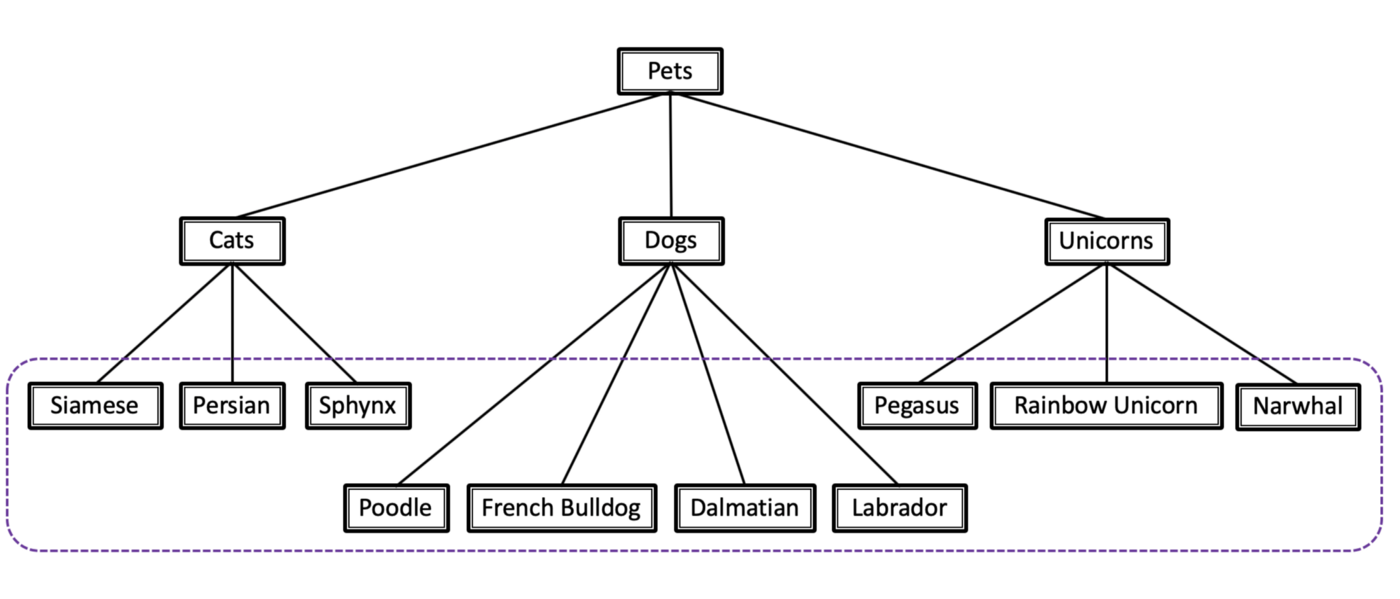
\includegraphics[width=1\textwidth]{images/weiss2019/hierarchical_class_flat.png}
    % 	\caption{Plochý přístup klasifikace hierarchické struktury\cite{weiss2019}}\label{fig:weiss2019flat}
    % \end{figure}

    \item Globální klasifikace
    
    Globální klasifikace spočívá v navržení jednoho komplexního--globálního modelu pro podchycení celé hierarchie jako celku. Jednotlivé implementace se mohou velice lišit. Globální model může být založen na tzv. \uv{clusterování}, multi-label klasifikaci nebo různě zkombinovaných algoritmů uzpůsobených na konkrétní případ užití.
    % Obrázek \ref{fig:weiss2019global} znázorňuje tento přístup.
    
    % \begin{figure}\centering
    % 	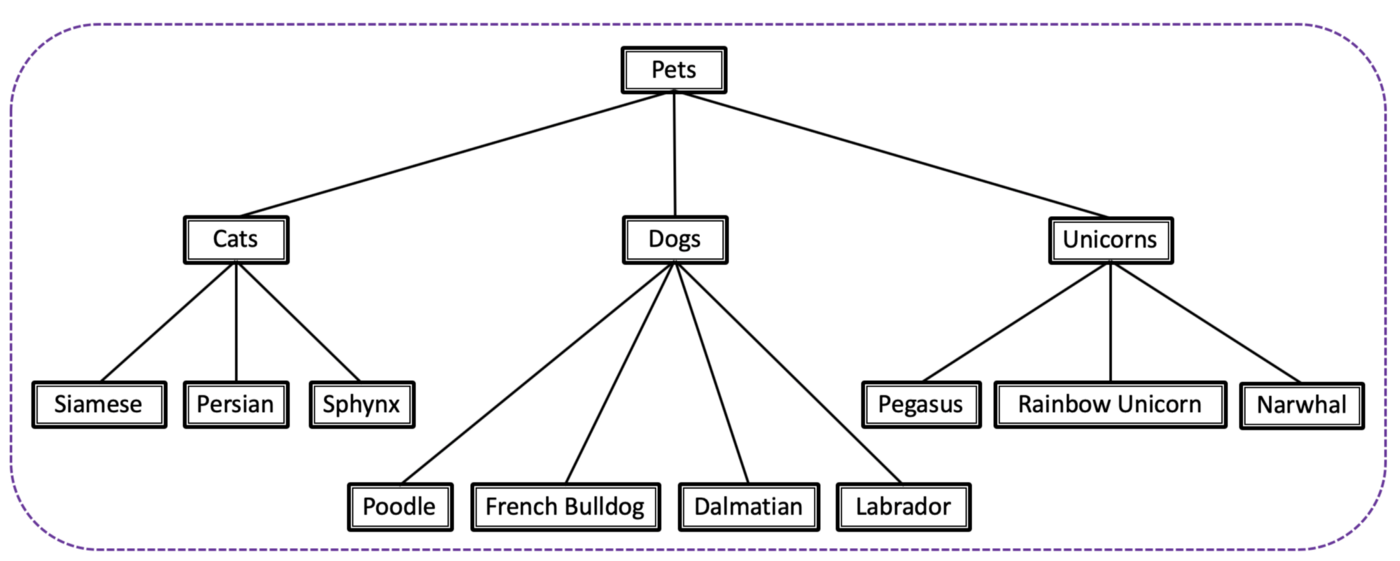
\includegraphics[width=1\textwidth]{images/weiss2019/hierarchical_class_global.png}
    % 	\caption{Globální přístup klasifikace hierarchické struktury\cite{weiss2019}}\label{fig:weiss2019global}
    % \end{figure}
    
    \item Hierarchicky strukturovaná lokální klasifikace
    
    Tento přístup se zakládá na myšlence použití několika oddělených klasifikátorů pro různé pozice ve struktuře. Existují tři možnosti, jak tento přístup implementovat:
    \begin{itemize}
        \item Lokální klasifikátor pro každý uzel předka
        
        Pro každý z vnitřních uzlů se natrénuje multi-label klasifikátor pro odlišení tříd jeho potomků. Tento přístup jde vyladit tak, aby se klasifikovaly jen relevantní třídy pro daný uzel a nedocházelo k chybným klasifikacím sourozeneckých tříd. Znázornění přístupu je zobrazeno na obrázku \ref{fig:weiss2019local1}.
    
        \begin{figure}\centering
        	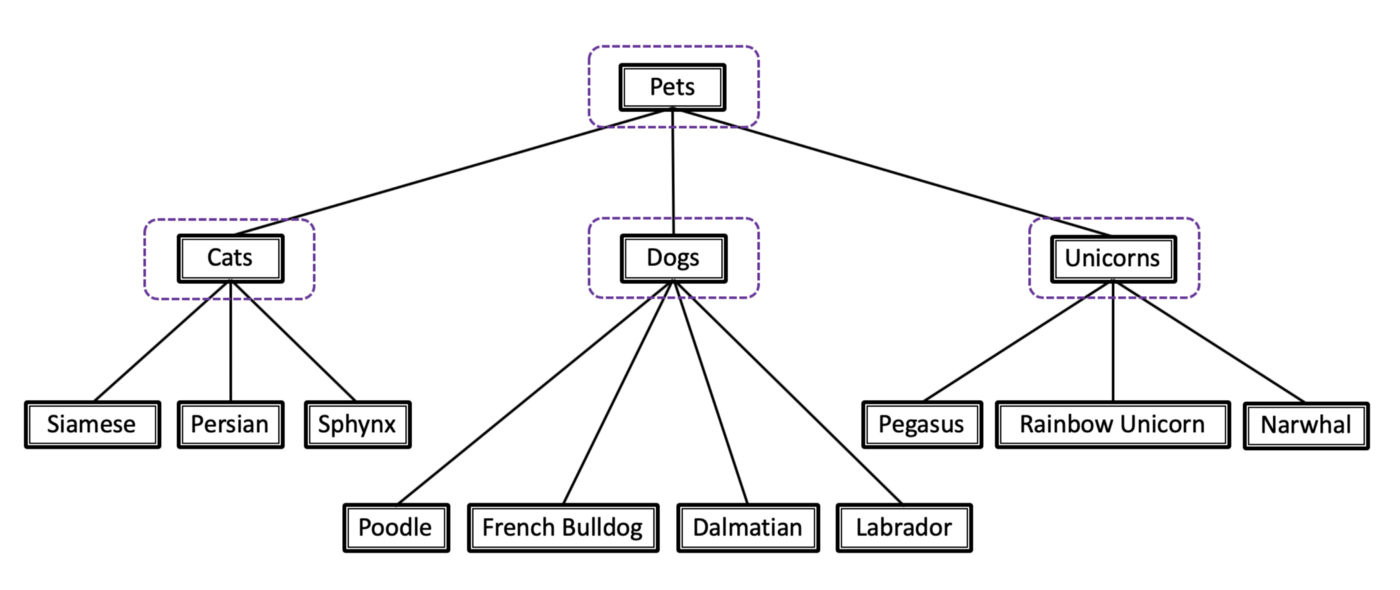
\includegraphics[width=1\textwidth]{images/weiss2019/hierarchical_class_local1.png}
        	\caption{Lokální klasifikátor pro každý uzel předka\cite{weiss2019}}\label{fig:weiss2019local1}
        \end{figure}
        
        \item Lokální klasifikátor pro každý uzel
        
        Přístup se zakládá na vytvoření binárního klasifikátoru pro každý uzel struktury (kromě kořenu). Oproti předchozímu přístupu lokální klasifikátory odpovídají na otázku \uv{Odpovídá tato třída instanci?} místo otázky \uv{Která z následujících tříd instanci odpovídá?} Tato metoda je zachycena na obrázku \ref{fig:weiss2019local2}.
    
        \begin{figure}\centering
        	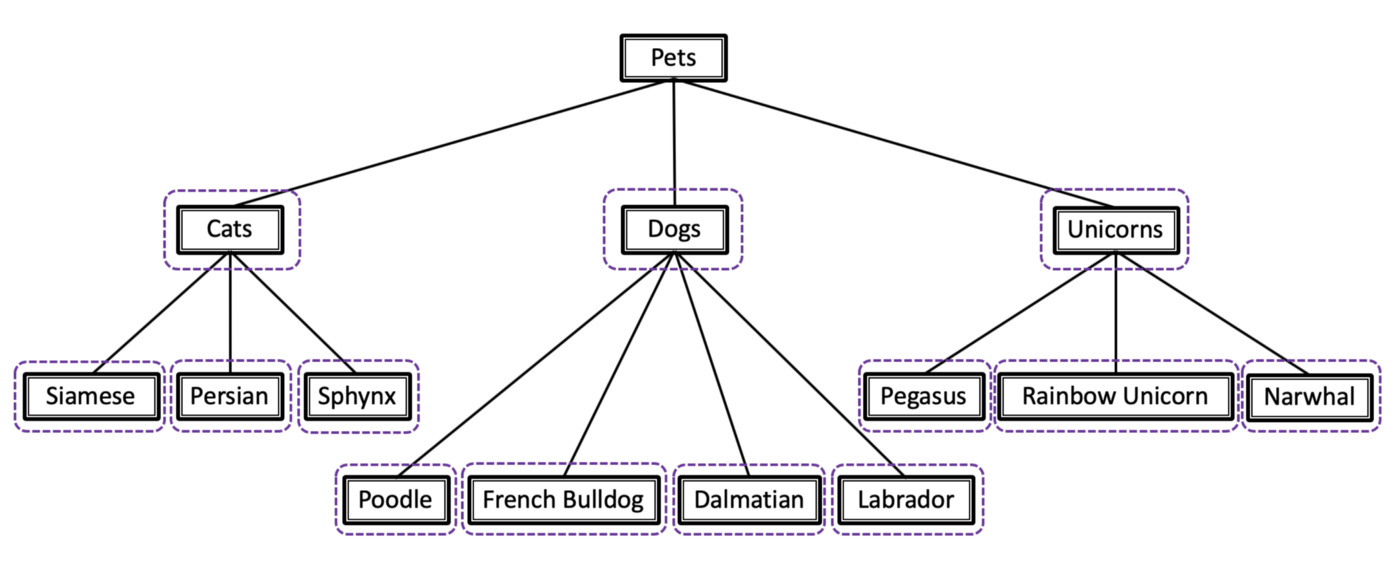
\includegraphics[width=1\textwidth]{images/weiss2019/hierarchical_class_local2.png}
        	\caption{Lokální klasifikátor pro každý uzel\cite{weiss2019}}\label{fig:weiss2019local2}
        \end{figure}

        \item Lokální klasifikátor pro každou úroveň
        
        U tohoto přístupu se množství klasifikátorů omezuje na počet úrovní hierarchické struktury. Z principu zde může docházet k nesmyslným klasifikacím sourozeneckých tříd. Přístup je zobrazen na obrázku \ref{fig:weiss2019local3}.
    
        \begin{figure}\centering
        	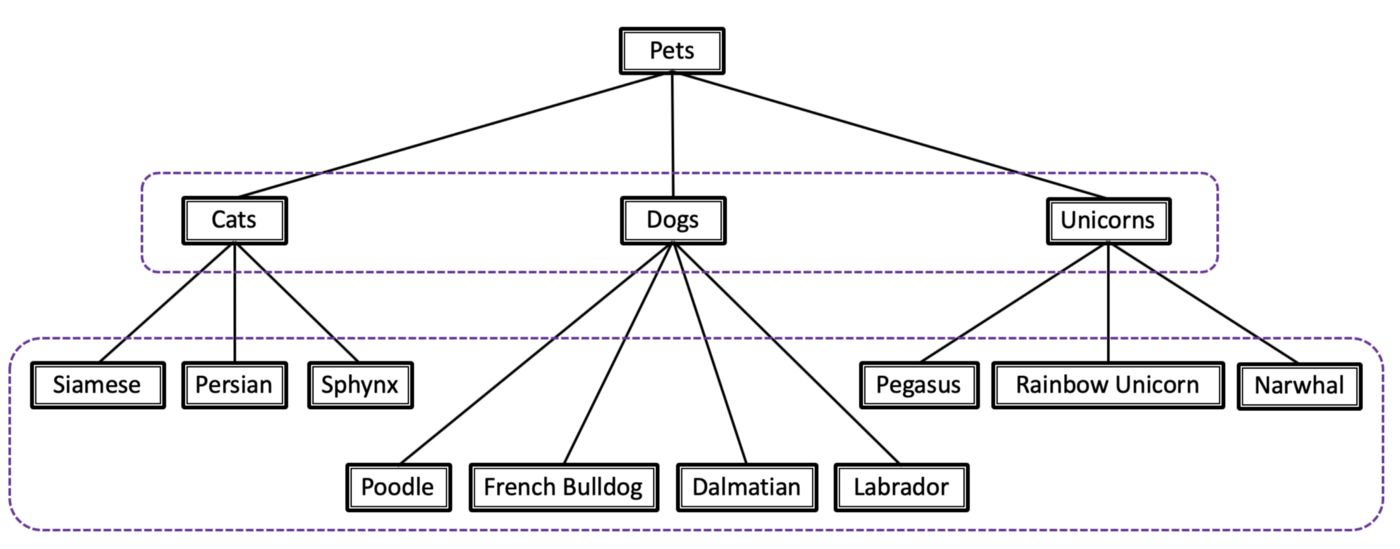
\includegraphics[width=1\textwidth]{images/weiss2019/hierarchical_class_local3.png}
        	\caption{Lokální klasifikátor pro každou úroveň\cite{weiss2019}}\label{fig:weiss2019local3}
        \end{figure}
    \end{itemize}
    
    Přístup pomocí lokálních klasifikátorů je intuitivní a ponechává hierarchickou informaci za použití standardních klasifikátorů. Může se ovšem projevit problém se zpětnou propagací chyb, která v základní implementaci mezi jednotlivými klasifikátory neprobíhá.
    
\end{enumerate}

\subsection{Multi-label klasifikace}
\label{sec:multilabel_classification}

Multi-label klasifikace je úloha \uv{přiřazování} jednotlivých tříd (příznaků) dané instanci. Třídy jedné instance tak nejsou vzájemně výlučné, na rozdíl od tzv. \uv{multi-class} klasifikace, ve které jde o úlohu \uv{rozřazování} jednotlivých instancí do tříd.

Existuje několik přístupů řešení multi-label klasifikace\cite{nooney2018}:

\begin{enumerate}
    \item Jeden z několika
    
    Přístup \uv{jeden z několika} v podstatě převádí problém multi-label klasifikace na standardní multi-class tím, že pro každou třídu se vytvoří jeden klasifikátor a ve výsledku se vybírá třída toho klasifikátoru, který dosahuje největší jistoty.
    
    \item Binární přítomnost
    
    V tomto případě se vytváří binární klasifikátor pro každou třídu, přičemž ve výsledku se vybírají všechny třídy pozitivně klasifikované na svou přítomnost. Instanci tak nemusí být přiřazena ve výsledku žádná třída. Tato metoda nebere ohled na vzájemné vazby mezi třídami.
    
    \item Řetězec klasifikátorů
    
    Přístup spočívá ve vytvoření řetězce klasifikátorů, kde každý jednotlivý klasifikátor využívá výsledků jemu předcházejících klasifikátorů. Tato metoda je schopná podchytit vazby mezi třídami. Počet jednotlivých klasifikátorů je opět rovný počtu tříd, ale trénování je sofistikovanější, jako je zobrazeno na obrázku \ref{fig:nooney2018multiclass}.

    \begin{figure}\centering
    	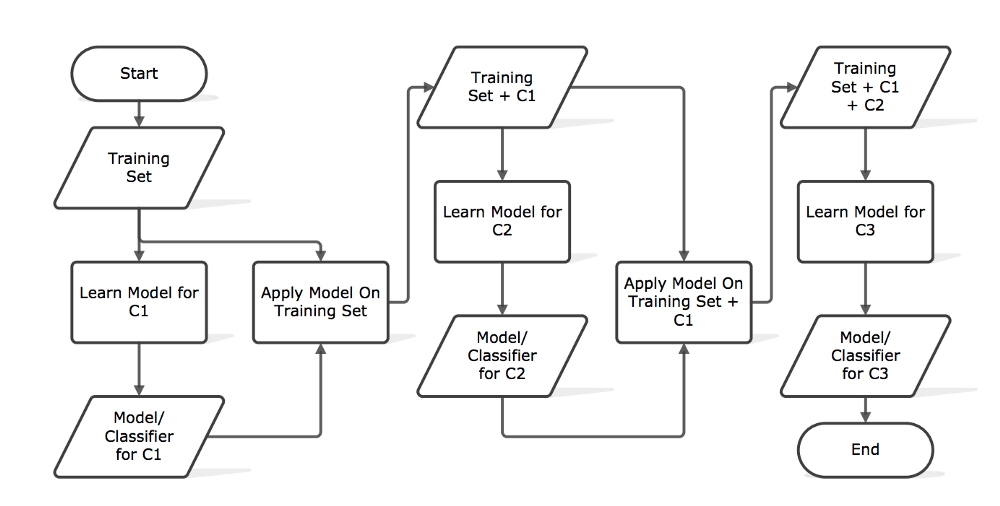
\includegraphics[width=1\textwidth]{images/nooney2018_multilable.png}
    	\caption{Schéma trénování řetězového multi-label klasifikátoru\cite{nooney2018}}\label{fig:nooney2018multiclass}
    \end{figure}
    
    \item Podmnožiny tříd
    
    Přístup zakládající se na podmnožinách celého setu tříd je také schopný podchycovat vztahy mezi třídami. Vytvoří se klasifikátor pro každou z umělých tříd odvozených jako podmnožiny původních tříd. U této metody dochází k problému tzv. \uv{kombinatorické exploze}, kdy úlohu nelze technologicky dořešit.
    
    \item Adaptivní algoritmy
    
    Metoda adaptivních algoritmů spočívá v uzpůsobování \uv{single-label} klasifikačních algoritmů na multi-label změnou jejich základních funkcí. Více ve zdrojovém článku\cite{nooney2018}.
    
\end{enumerate}

\subsection{Analýza CPV kódů v datech}
\label{sec:cpv_distribution}

Jedním ze základních kroků data science projektů předcházejících samotnému budování modelu je analýza dat. Tuto kapitolu tak věnuji statistické analýze CPV kódů v datech VZ.

Dataset s přiřazenými CPV kódy k zakázkám mi byl poskytnut správci portálu Hlídač státu. Obsahuje přes 30 tisíc záznamů párů evidenčních čísel zakázek(dále jen ECZ\footnote{Evidenční čísla zakázky jsou identifikátory zakázek používané ve Věstníku. Napříč profily zadavatelů ovšem zpravidla používané nejsou.}) a jim přiřazené CPV kódy. Zakázky datasetu jsou náhodně vybrané zakázky s uvedeným ECZ(zhruba pětina ze všech zakázek) za období leden až červen 2019 od více než tisíce různých zadavatelů z celé České republiky. Majoritní zastoupení (přes 12 tisíc zakázek) má samotný zadavatel Jihočeského kraje a druhý nejpočetnější je zadavatel Libereckého kraje s jedním tisícem zakázek. Nad 500 zakázek v datasetu dosahují ještě další 4 zadavatelé.

Některé ECZ se v datasetu vyskytují mnohonásobně, zatímco jiné nemají přiřazený žádný CPV kód a některé mají kódy nevalidní. Dataset tak čistím pro ponechání pouze validních záznamů. Ve výsledku tak zbývá 10\,607 607namů párů kódů ECZ--CPV obsahujících 9127 unikátních ECZ kódů (počet zakázek) a 1756 unikátních kódů CPV.

V tabulce \ref{table:CPVdist} zaznamenávám hodnoty distribuce CPV kódů v datasetu. Na diagramech odkázaných z tabulky jsou zobrazeny odpovídající distribuce relevantních tříd:
\begin{table}[h!]
\centering
    \begin{tabular}{|l|r|r|r|}
         \hline
          Úroveň & Počet unikátních & Počet relevantních* & Diagram\\\hline
          \hline
          Oddíly & 44 & 19 & \ref{fig:cpvdist1} \\\hline
          Skupiny & 245 & 21 & \ref{fig:cpvdist2} \\\hline
          Třídy & 636 & 17 & --- \\\hline
          Kategorie & 1134 & 9 & --- \\\hline
          Celý kód & 1756 & 8 & \ref{fig:cpvdist} \\\hline
    \end{tabular}
\caption[Přehledová tabulka distribuce úrovní CPV kódů v datasetu]{Přehledová tabulka distribuce úrovní CPV kódů v datasetu;\newline*~za relevantní třídy beru takové, které mají alespoň 100 výskytů}
\label{table:CPVdist}
\end{table}

\begin{figure}\centering
	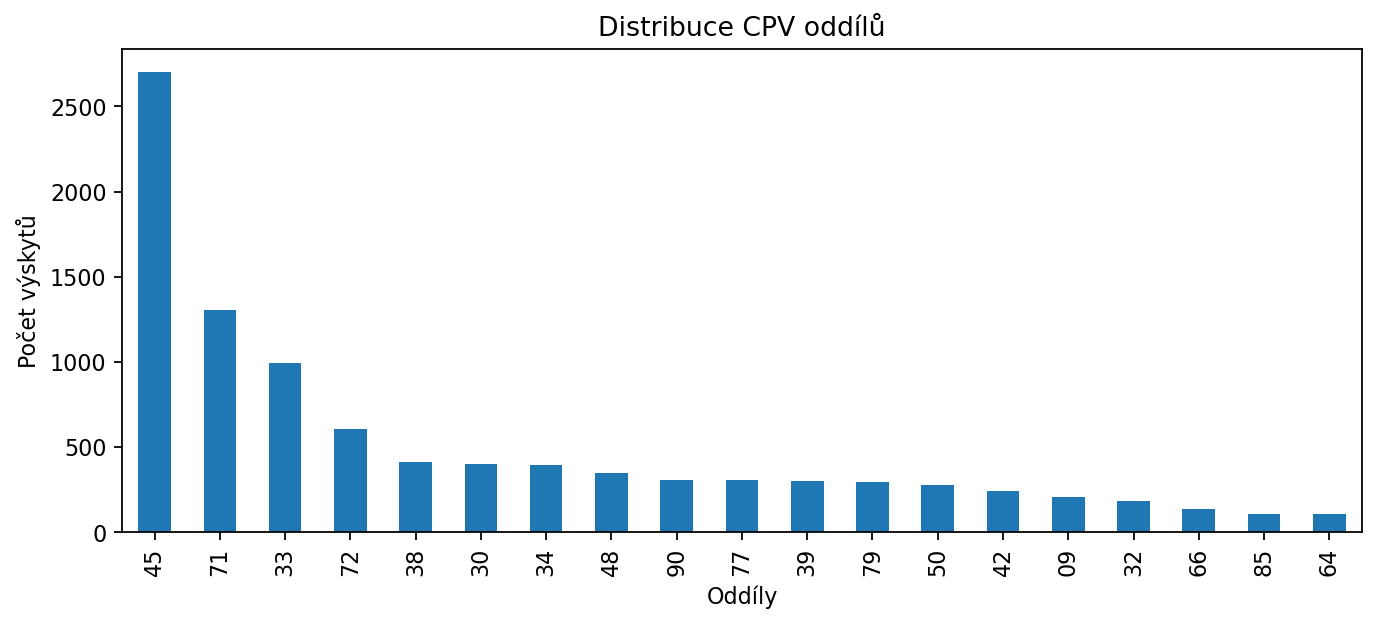
\includegraphics[width=1\textwidth]{images/cpv/dist_cpv_1.png}
	\caption{Distibuce CPV oddílů v datasetu}\label{fig:cpvdist1}
\end{figure}
\begin{figure}\centering
	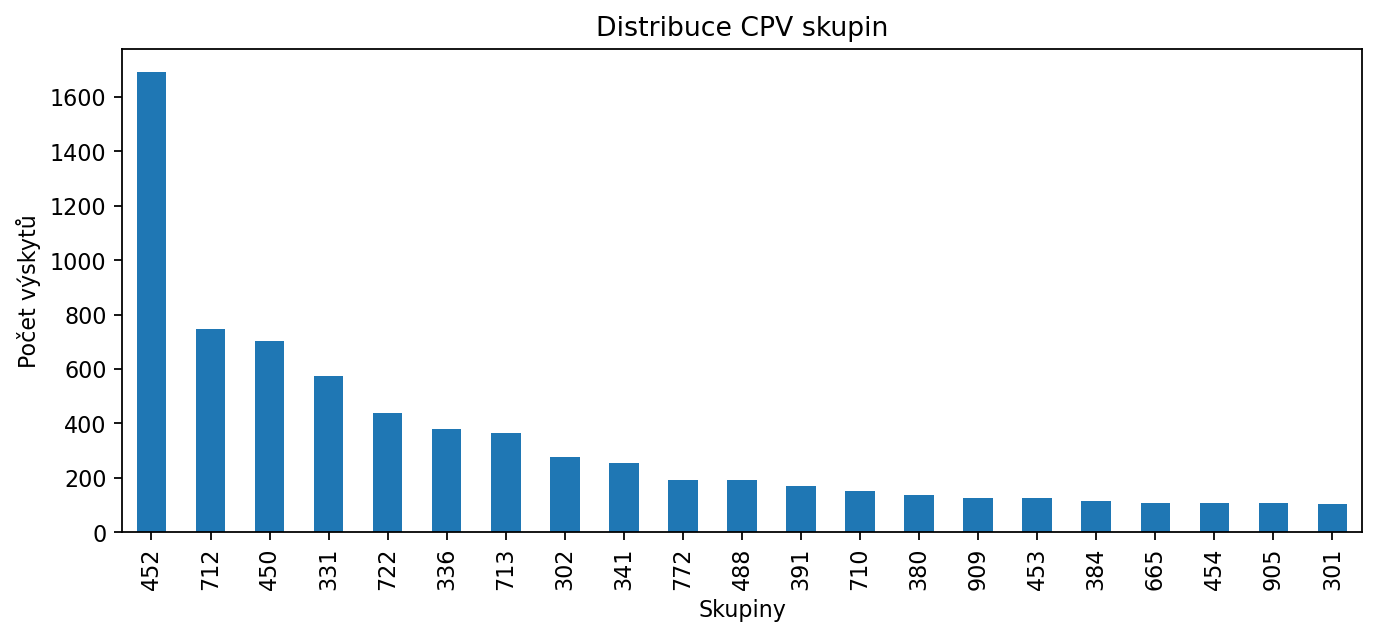
\includegraphics[width=1\textwidth]{images/cpv/dist_cpv_2.png}
	\caption{Distibuce CPV skupin v datasetu}\label{fig:cpvdist2}
\end{figure}
% \begin{figure}\centering
% 	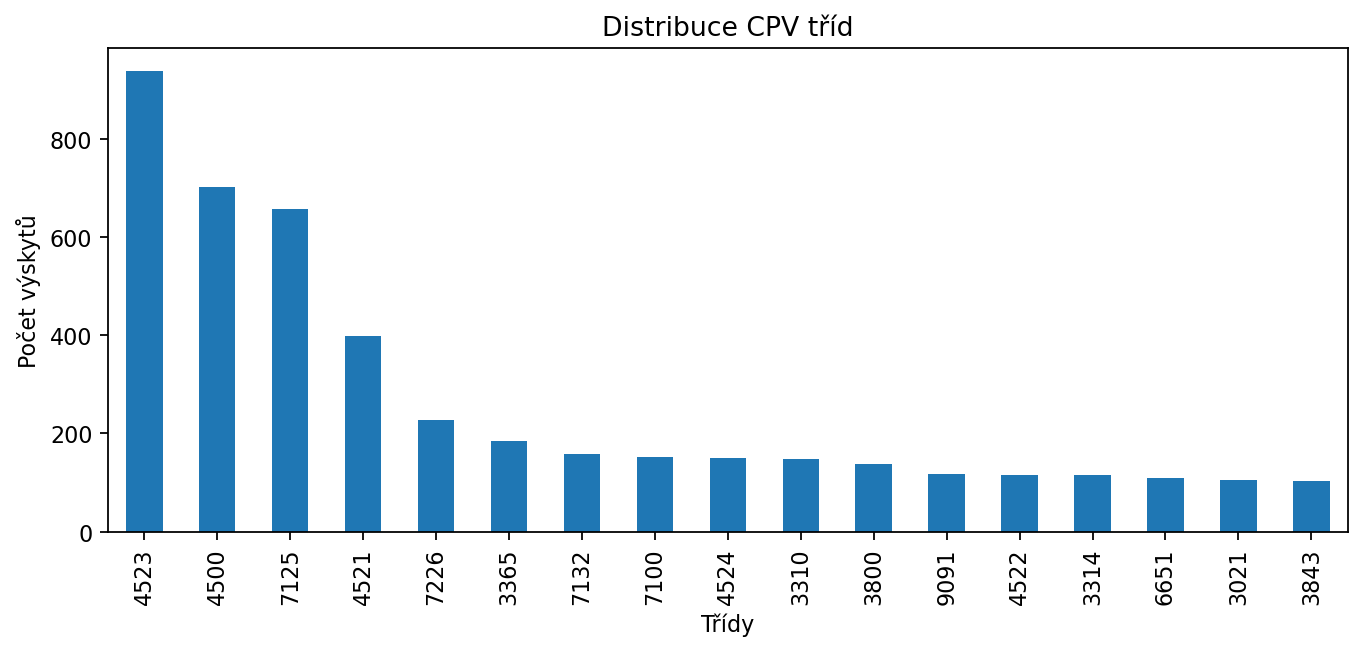
\includegraphics[width=1\textwidth]{images/cpv/dist_cpv_3.png}
% 	\caption{Distibuce CPV tříd v datasetu}\label{fig:cpvdist3}
% \end{figure}
% \begin{figure}\centering
% 	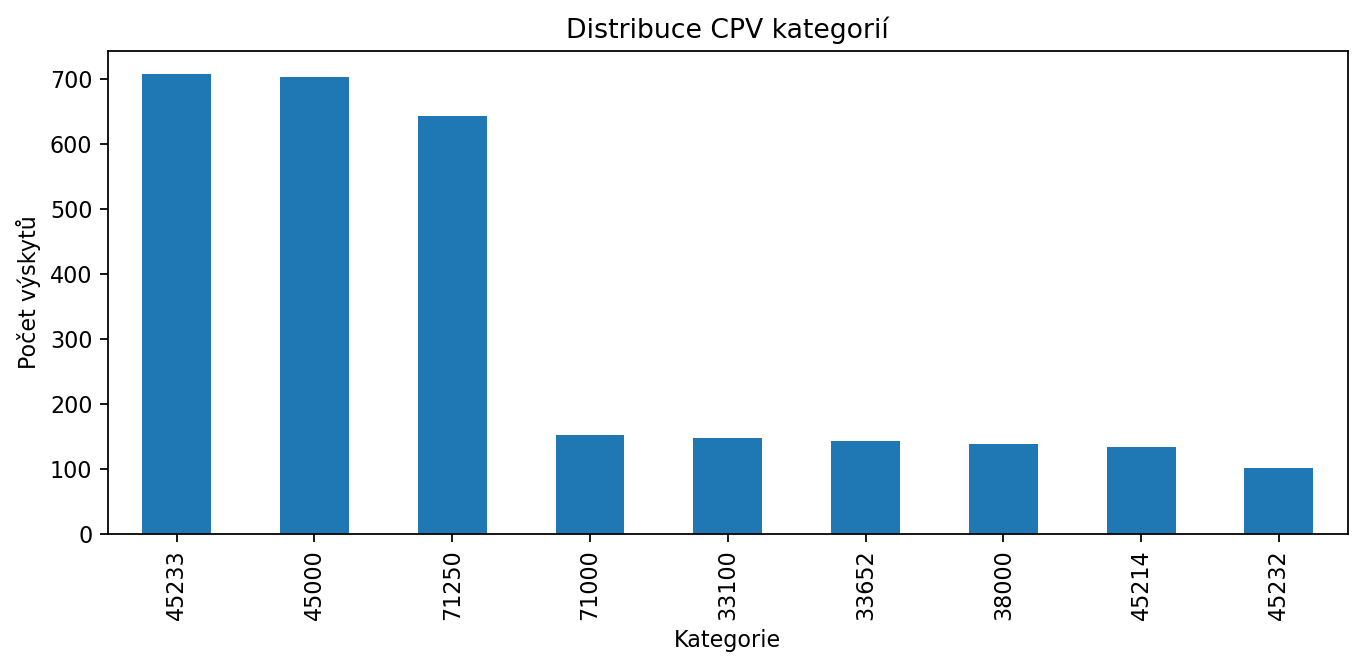
\includegraphics[width=1\textwidth]{images/cpv/dist_cpv_4.png}
% 	\caption{Distibuce CPV kategorií v datasetu}\label{fig:cpvdist4}
% \end{figure}
\begin{figure}\centering
	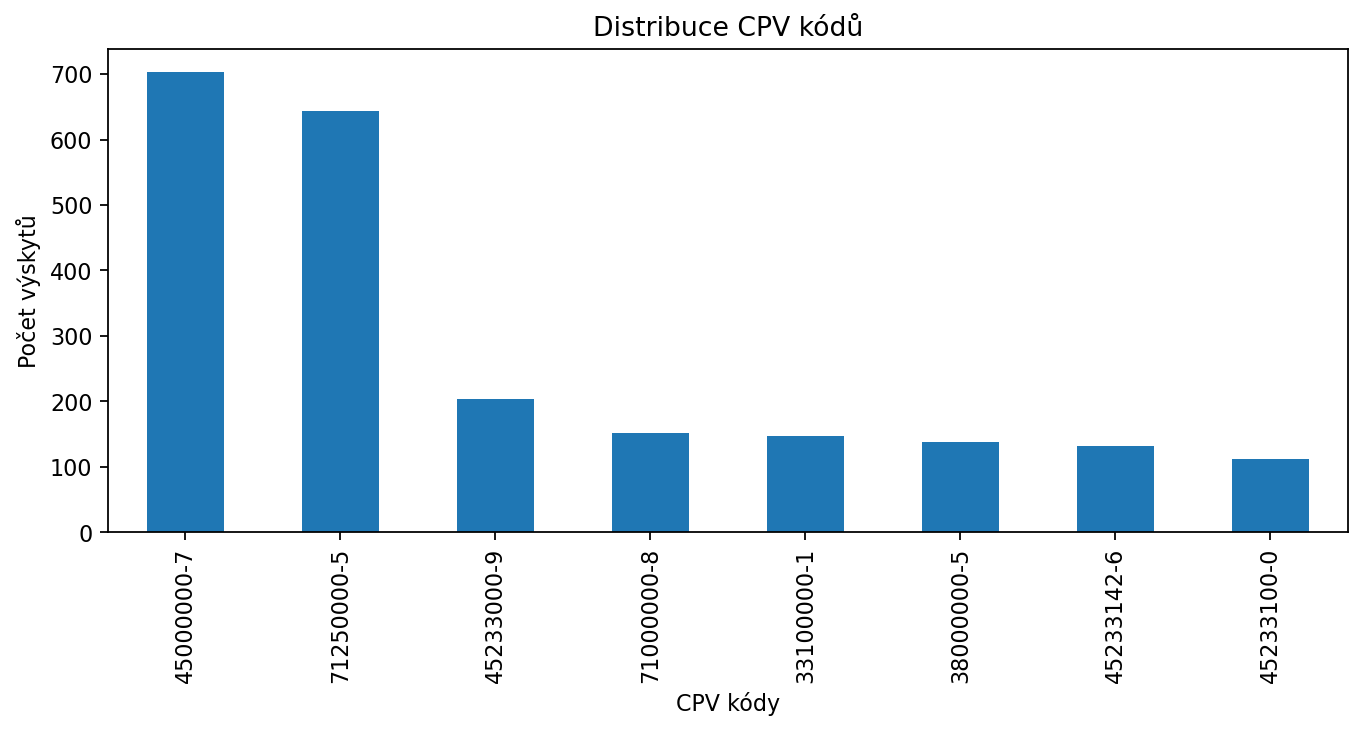
\includegraphics[width=1\textwidth]{images/cpv/dist_cpv.png}
	\caption{Distibuce CPV kódů v datasetu}\label{fig:cpvdist}
\end{figure}
    
Z hodnot v tabulce \ref{table:CPVdist} a diagramů \ref{fig:cpvdist1}, \ref{fig:cpvdist2} a \ref{fig:cpvdist} je zřejmé, že zastoupení tříd je nevyrovnané. Zatímco zakázky týkající se stavebního odvětví (oddíl 45) tvoří signifikantní majoritu, některé oddíly nemají zastoupení vůbec (oddíl 41 – Shromážděná a upravená voda). Relevantních\footnote{\label{not:relevant_class}Relevantní -- třídy se zastoupením alespoň 100 výskytů} tříd je necelá polovina.

Vzhledem k celkovému počtu CPV kódů (necelých 10 tisíc) oproti počtu unikátních kódů v datasetu (1756) je zřejmé, že konkrétních kódů chybí veliké množství. Pouhých 8 z nich potom čítá více než 100 výskytů.

Je možné si povšimnout, že některé oddíly samy o sobě obsahují hned několik relevantních skupin, což vysvětluje vyšší počet relevantních skupin oproti počtu relevantních oddílů. Tento jev je potom vidět na diagramu \ref{fig:cpvdist2}, kde je hned několik skupin z oddílů 45, 71, 33 a 30.

Diagram \ref{fig:cpvdist} potom ukazuje, že mnoho zakázek má uvedené CPV zařazení v nejmenším možném detailu, což potvrzuje počet výskytů kódů 45000000-7, 71000000-8 a 38000000-5.

Na základě zjištění analýzy datasetu usuzuji, že trénovat úspěšně klasifikátor pro určení CPV zařazení zakázek podle textu jejich dokumentace by na množině zakázek tohoto datasetu nebylo možné. Pro smysluplné učení klasifikátoru by dataset musel být mnohem obsáhlejší a vyvážený v zastoupení jednotlivých tříd.

\subsection{Extrakce CPV kódů}
\label{sec:cpv_extraction}

Přestože v systému neaplikuji automatickou klasifikaci dokumentů, některé CPV kódy lze získat přímo z dokumentů.

Pro tyto účely implementuji extraktor CPV kódů z textu, který podle regulárního výrazu vyhledává  všechny řetězce odpovídající formátu CPV kódu.

\newpage
\section{Embedding dokumentů}
\label{sec:document_embedding}
Dnešní digitální výpočetní technologie spoléhají bez výjimky na číselnou reprezentaci dat. Některá data je možné přirozeným způsobem zobrazovat do spojitého prostoru, jako například obraz reprezentovaný dvourozměrným popisem barev, či zvuk popsaný průběhem signálu, zatímco jiná data takto přirozeně reprezentovat nelze.

Jedním z obtížně reprezentovatelných typů dat je text přirozeného jazyka, kde se pro reprezentaci slov při jeho zpracování tradičně užívá kód 1 z n, který z principu vytváří velmi řídce obsazené prostory s vysokým počtem dimenzí. To je z mnoha důvodů nepraktické. Data jsou prostorově náročná a reprezentace nijak nezachycuje vztahy mezi slovy.

Žádoucí je tak převést všechna slova do spojitého prostoru pevně dané dimenze, která nebude závislá na velikosti slovníku.

V praxi se používají vektory v prostoru reálných čísel nabývajícím desítky až stovky rozměrů. Vnoření jsou vytvářena automaticky, často s použitím strojového učení, čímž se význam jednotlivých rozměrů stává neinterpretovatelný. Vektory tak mají význam pouze ve vztahu k ostatním, samostatně ne.

\subsection{Embedding}
Ve svém článku Palachy\cite{palachy2019} shrnuje vnořování slov (dále angl. embedding), jako metodu reprezentace slov v číselném vektorovém prostoru, která se stala nedílnou součástí dnešních řešení úloh strojového zpracování přirozeného jazyka (dále NLP z angl. natural language processing). Embedding umožňuje modelům strojového učení závisejícím na vektorové reprezentaci vstupu využít takové reprezentace jako bohatšího vyjádření samotného vstupního textu. Ve vektorovém prostoru je možné zachovat více sémantické i syntaktické informace, což napomáhá k dosažení lepších výsledků v téměř kterékoli úloze zpracování přirozeného jazyka.

Milníkem se stala v roce 2013 publikace práce skupiny Tomáše Mikolova. Jejich word2vec model s inovativním přístupem k získávání embeddingů spustil vlnu zájmu o obor. 
Palachy dodává, že myšlenka embeddingu a její zásadně pozitivní dopady vedly vědce k úvaze o její aplikaci na větší textové celky, od vět až po knihy. Snaha mnoha lidí vyústila v řadu nových metod získávání vektorové reprezentace s různými inovativními řešeními a další významné průlomy v oboru.
Ve článku \cite{palachy2019} člení přístupy řešení text embeddingu do čtyř kategorií.

1.	Sumarizace slovních vektorů

Klasický přístup, který zastupuje například algoritmus „bag-of-words“ v případě „one-hot“ slovních vektorů. Je možné aplikovat různá schémata vážení k sumarizaci vektorů.

2.	Modelování témat

Přestože zde nelze mluvit o získávání embeddingů jako o hlavním účelu, modelovací techniky jako LDA („latent Dirichlet allocation“) nebo PLSI („probabilistic latent semantic indexing“) inherentně generují prostor pro embedding dokumentů. Tím modelují a vysvětlují distribuci slov v korpusu, kde jednotlivé dimenze mohou být viděny jako latentní sémantické struktury skryté v datech.

3.	Enkodér---dekodér modely

Přístup využívající vnitřní reprezentaci dat v podobě číselných vektorů. Modely vznikají učením bez učitele s výhodou použití stále dostupnějších velkých korpusů s neoznačenými daty.

4.	Učení s učitelem

Modely neuronových sítí mají schopnost naučení získávat obohacené reprezentace vstupních dat, které využívají k řešení úloh souvisejících s textem. Takto naučené sítě obsahují skryté vrstvy, kde jsou data reprezentovaná právě číselnými vektory.

\subsubsection{Klasické metody}
\subsubsection*{Bag-of-words}
Metoda reprezentující text jako (multi)množiny vyskytujících se slov -- tzv. „bag-of-words“ (dále BOW). Každý dokument je zastoupen vektorem o délce velikosti slovníku, kde každá pozice zastupuje počet výskytů daného slova. Z~této podstaty metoda neuchovává žádnou gramatickou ani souslednou informaci o textu. Viz. obrázek \ref{fig:palachy2019BOW}.
\begin{figure}\centering
	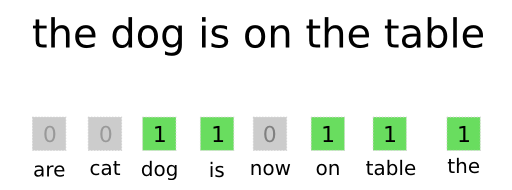
\includegraphics[width=0.5\textwidth]{images/palachy2019/palachy2019_BOW.png}
	\caption{Příklad reprezentace BOW\cite{palachy2019}}\label{fig:palachy2019BOW}
\end{figure}

\subsubsection*{Bag-of-n-grams}
Metoda se snaží oproti klasickému BOW omezit ztrátu informace o pořadí. Místo výskytu slov tak počítá výskyty n--slovných sousloví. Klasický BOW je tak případ této metody pro n = 1. Hlavní problém této metody je nelineární závislost velikosti slovníku na počtu unikátních slov. Proto se často užívají techniky ke snížení velikosti slovníku. Viz. obrázek \ref{fig:palachy2019BONG}.
\begin{figure}\centering
	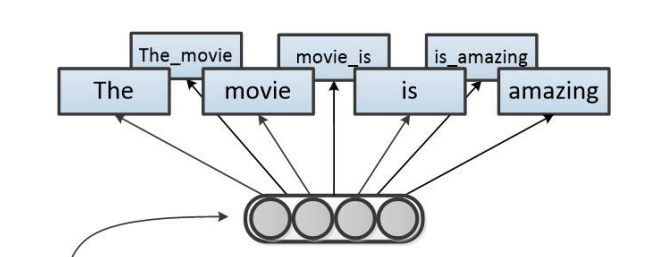
\includegraphics[width=0.5\textwidth]{images/palachy2019/palachy2019_BONG.png}
	\caption{Schéma reprezentace bag-of-n-grams\cite{palachy2019}}\label{fig:palachy2019BONG}
\end{figure}

\subsubsection*{tf-idf}
Předešlé metody počítají jednotlivé výskyty, což není zcela objektivní metrika, protože některá slova se vyskytují obecně častěji, čímž se stávají méně důležitými. Alternativou je vážící schéma „term frequency – inverse document frequency“ (dále \textit{tf-idf}). Toto schéma se skládá ze dvou složek: četnost slova v dokumentu (\textit{tf}) a převrácená četnost slova ve všech dokumentech (\textit{idf}). Pro výsledné ohodnocení se složky násobí, přičemž ve výpočtu \textit{tf} roste s počtem výskytů, zatímco \textit{idf} je vysoké, když je slovo vzácné.

\subsubsection{Modelování témat}
\subsubsection*{Latent Dirichlet allocation}
LDA je generativní statistický model opírající se o myšlenku, že „každý dokument lze popsat distribucí témat a každé téma může být popsáno distribucí slov“. Při vytváření modelu z korpusu dokumentů vzniká skrytá (latentní) vrstva abstraktních témat. Každý dokument je poté reprezentován jako výběr z Dirichletova rozdělení nad tématy a každé téma jako výběr z Dirichletova rozdělení nad slovy. Hlavním užitím LDA je neřízené odhalování témat v dokumentech, tzv. modelování témat (z angl. topic modelling). Existují avšak i užití, kde latentní prostor témat se využívá jako prostor pro embedding dokumentů. Viz. obrázek \ref{fig:palachy2019LDA}.
\begin{figure}\centering
	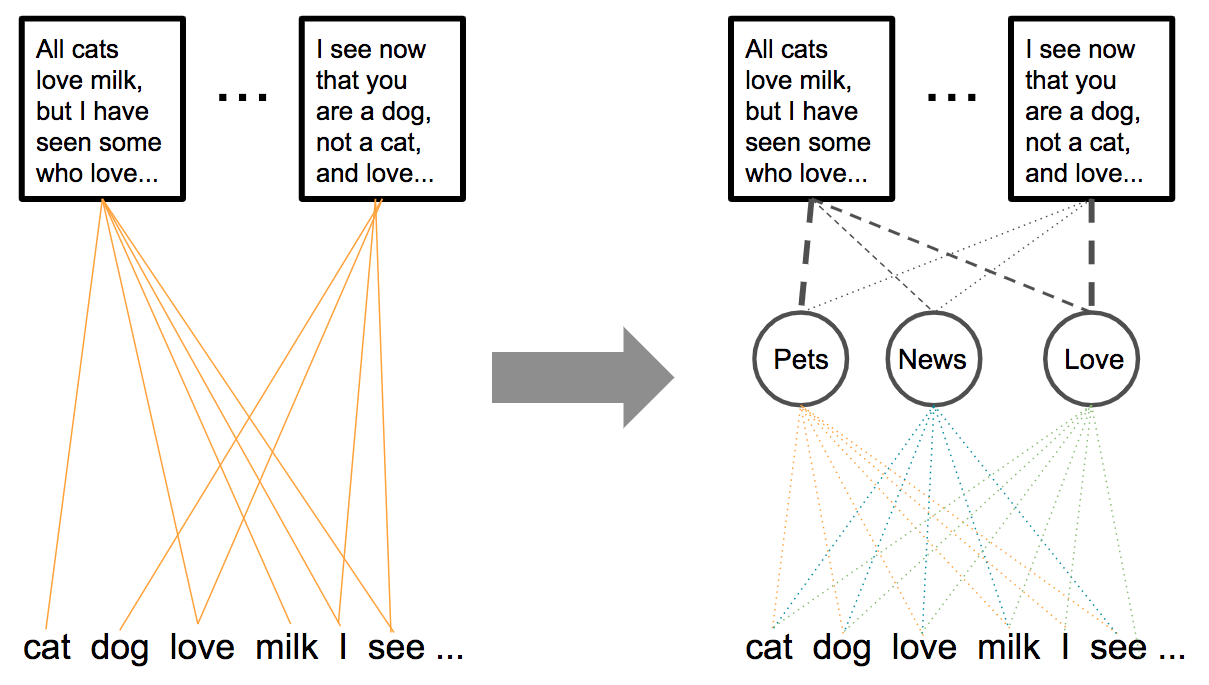
\includegraphics[width=0.8\textwidth]{images/palachy2019/palachy2019_LDA.png}
	\caption{Ukázka přechodu z BOW na LDA\cite{palachy2019}}\label{fig:palachy2019LDA}
\end{figure}

\newpage
\subsubsection{Metody učení bez učitele}
Většina modelů text embeddingu byla navržena na základě myšlenky distribuční hypotézy (z angl. The Distributional Hypothesis), podle které slova vyskytující se ve stejných kontextech tíhnou k podobnému významu. Tuto myšlenku o slovech modely dále rozšiřuji různými přístupy i pro delší části textu.

\subsubsection*{word2vec}
Jak už bylo řečeno v úvodní kapitole, word2vec\cite{mikolov2013} zaznamenal převrat v oboru zpracování přirozeného jazyka. Word2vec je mělká (dvouvrstvá) neuronová síť, která dokáže matematicky podchytit vazby mezi slovy z korpusu. Jako příklad úspěšného objevu se uvádí široce známá formule:
\begin{equation}
word2vec('king' ) - word2vec('man' ) + word2vec('woman' ) \cong word2vec('queen')
\end{equation}
Tvůrci modelu přichází se dvěma architekturami. První je CBOW (z angl. continuous bag-of-words), která predikuje prostřední slovo na základě několika okolních slov, zatímco druhá, tzv. skip-gram architektura, v jistém smyslu dělá opačný proces, tedy predikuje okolní kontextová slova na základě jednoho vstupního. Dle autorů je mezi architekturami výkonnostní rozdíl. Zatímco CBOW je rychlejší, architektura skip-gram dokáže predikovat lépe pro méně obvyklá slova\cite{mikolov2013}.
 Na obrázku \ref{fig:mikolov2013word2vec} jsou vidět obě architektury.
\begin{figure}\centering
	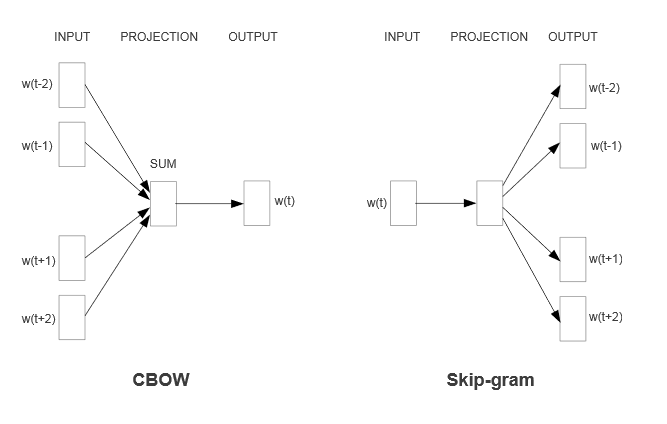
\includegraphics[width=0.8\textwidth]{images/mikolov2013_word2vec.png}
	\caption{Architektury CBOW a skip-gram\cite{mikolov2013}}\label{fig:mikolov2013word2vec}
\end{figure}

\newpage
\subsubsection*{n-gram embeddingy}
V práci \cite{mikolov2013b} autoři rozšiřují skip-gram algoritmus modelu word2vec pro použití na krátkých frázích. Místo jednoslovných tokenů tak při učení modelu používají několikaslovné fráze. Takový přístup je přirozeně nevhodný pro delší fráze kvůli rychlému růstu velikosti slovníku se zvyšující se délkou fráze. Metoda také negeneralizuje svou funkci na neznámé fráze jako jiné metody.

\subsubsection*{Agregace embeddingů slov}
Velice intuitivní metoda pro získání embeddingu delšího textu je agregace embeddingů jednotlivých slov. Provedením vektorové operace získáme opět vektor v tom samém embeddingovém prostoru. Nabízí se například sčítání či průměrování vektorů,  ale existují i o něco složitější řešení obsahující další kroky či vrstvy. Například v práci Kentera\cite{kenter2016} návrhli jednoduchou neuronovou síť nad průměrovanými slovními embeddingy, čímž predikuje okolní věty. Palachy uvádí ve svém článku\cite{palachy2019} další příklady.

\subsubsection*{doc2vec}
Model, zvaný jako „paragraph vectors“\cite{le2014}, je zřejmě první pokus zobecnění použití modelu word2vec na sekvence slov. Metoda je založená na rozšíření standardního modelu o paměťový vektor, který cílí na zachycení téma/kontextu ze vstupu. Každý odstavec je mapovaný na unikátní vektor (tzv. paragraph vector) podobně jako slova ze slovníku. Tento vektor je sdílený mezi všemi kontexty okna plovoucího přes odstavec. Pro predikované slovo se paměťový vektor přidává ke kontextu fixní velikosti. Vektory pro neznámé odstavce jsou náhodně inicializované. Paragraph vector je zobrazen na schéma \ref{fig:palachy2019PV}.
\begin{figure}\centering
	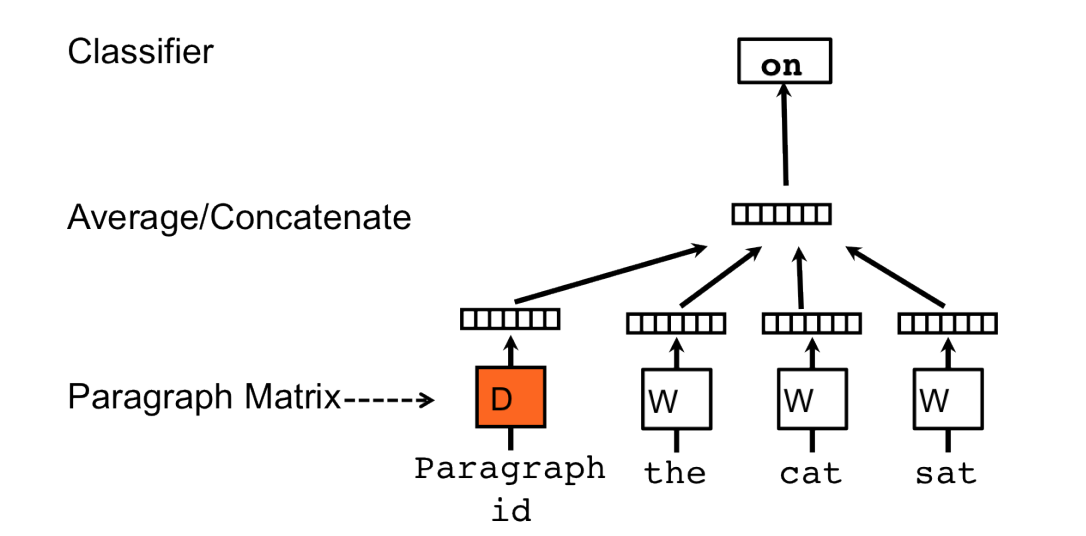
\includegraphics[width=0.8\textwidth]{images/palachy2019/palachy2019_PV.png}
	\caption{Sdílená paměť modelu paragraph vector\cite{palachy2019}}\label{fig:palachy2019PV}
\end{figure}

\subsubsection*{sent2vec}
Představený model sent2vec v Pagliardiniho\cite{pagliardini2018} práci dále kombinuje předešlé přístupy. Autoři rozšiřují CBOW algoritmus modelu word2vec o schopnost zpracování celých vět. Pro predikci slova ve větě je místo kontextového okna o fixní velikosti použito jako kontext celý zbytek věty. Vektory slov z kontextu jsou opět průměrované jako vstup do neuronové sítě. Schéma modelu je zobrazeno na obrázku \ref{fig:palachy2019sent2vec}.
\begin{figure}\centering
	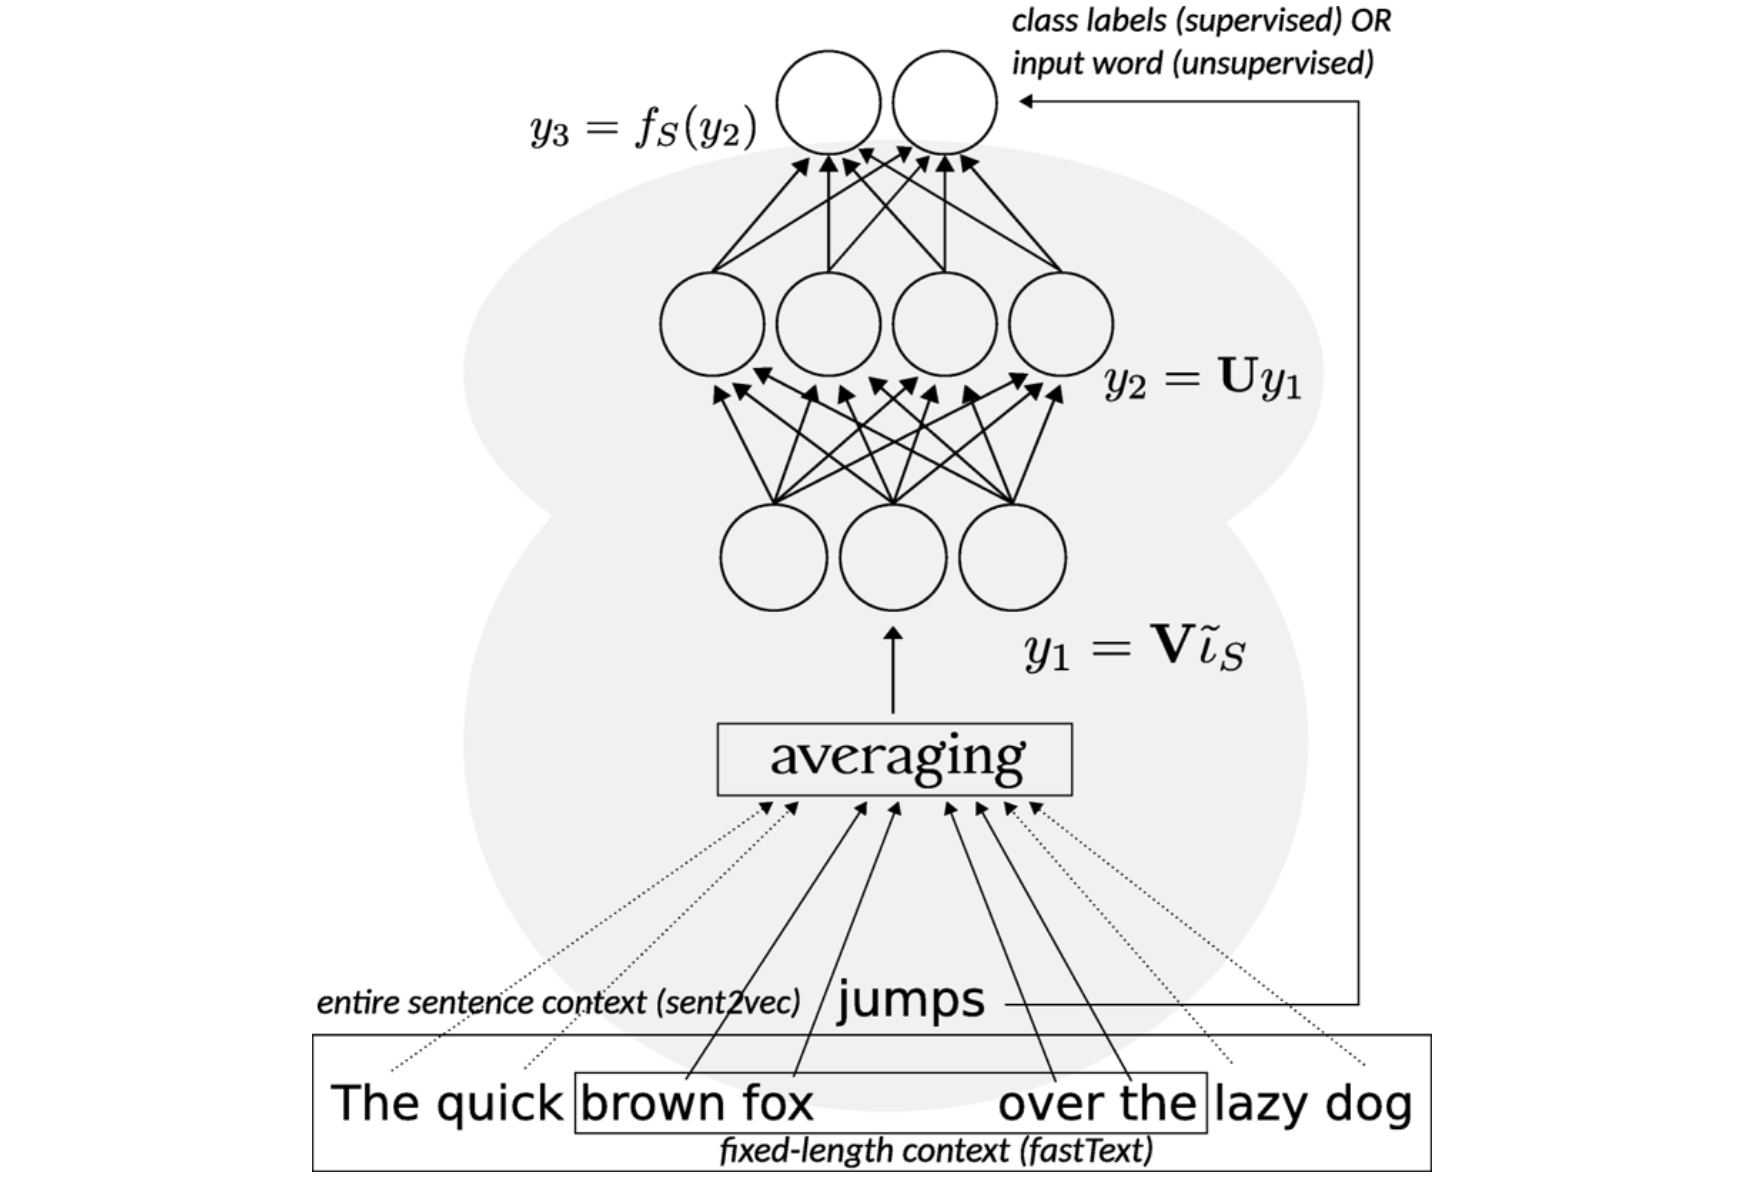
\includegraphics[width=\textwidth]{images/palachy2019/palachy2019_sent2vec.png}
	\caption{Schéma modelu sent2vec s příkladem\cite{palachy2019}}\label{fig:palachy2019sent2vec}
\end{figure}

\subsubsection*{GloVe}
V práci Penningtona\cite{pennington2014} přichází s odlišnou myšlenkou získávání informace pro embedding slov, kterou předznamenává jeho název odvozený z anglického „Global Vectors“. Zatímco word2vec model je zaměřen pouze na lokální informaci v textu (slova z okolí), GloVe vedle lokální zachycuje i globální statistiky korpusu. Ve výpočtech k tomu zahrnuje matici společných výskytů slov (z angl. co-occurrence matrix). Autorům se tak podařilo vytvořit další model, který předčil ostatní modely v úlohách rozpoznávání pojmenovaných entit, podobnosti či analogie slov.

Ve článku Ganegedara\cite{genegedara2019} je GloVe popsán dopodrobna.

\subsubsection*{Skip-thought vektory}
Další pokus o zobecnění skip-gram architektury word2vec modelu rozšiřuje původní koncept ve smyslu použití celé věty jako základní jednotky pro predikci. Skip-thought přístup predikuje předcházející a následující větu. Autoři používají rekurentní neuronové sítě pro enkodér a dekodér, které využívají embedovací vrstvu provádějící embedding jednotlivých slov. Více je vysvětleno na obrázku \ref{fig:palachy2019ST}.
\begin{figure}\centering
	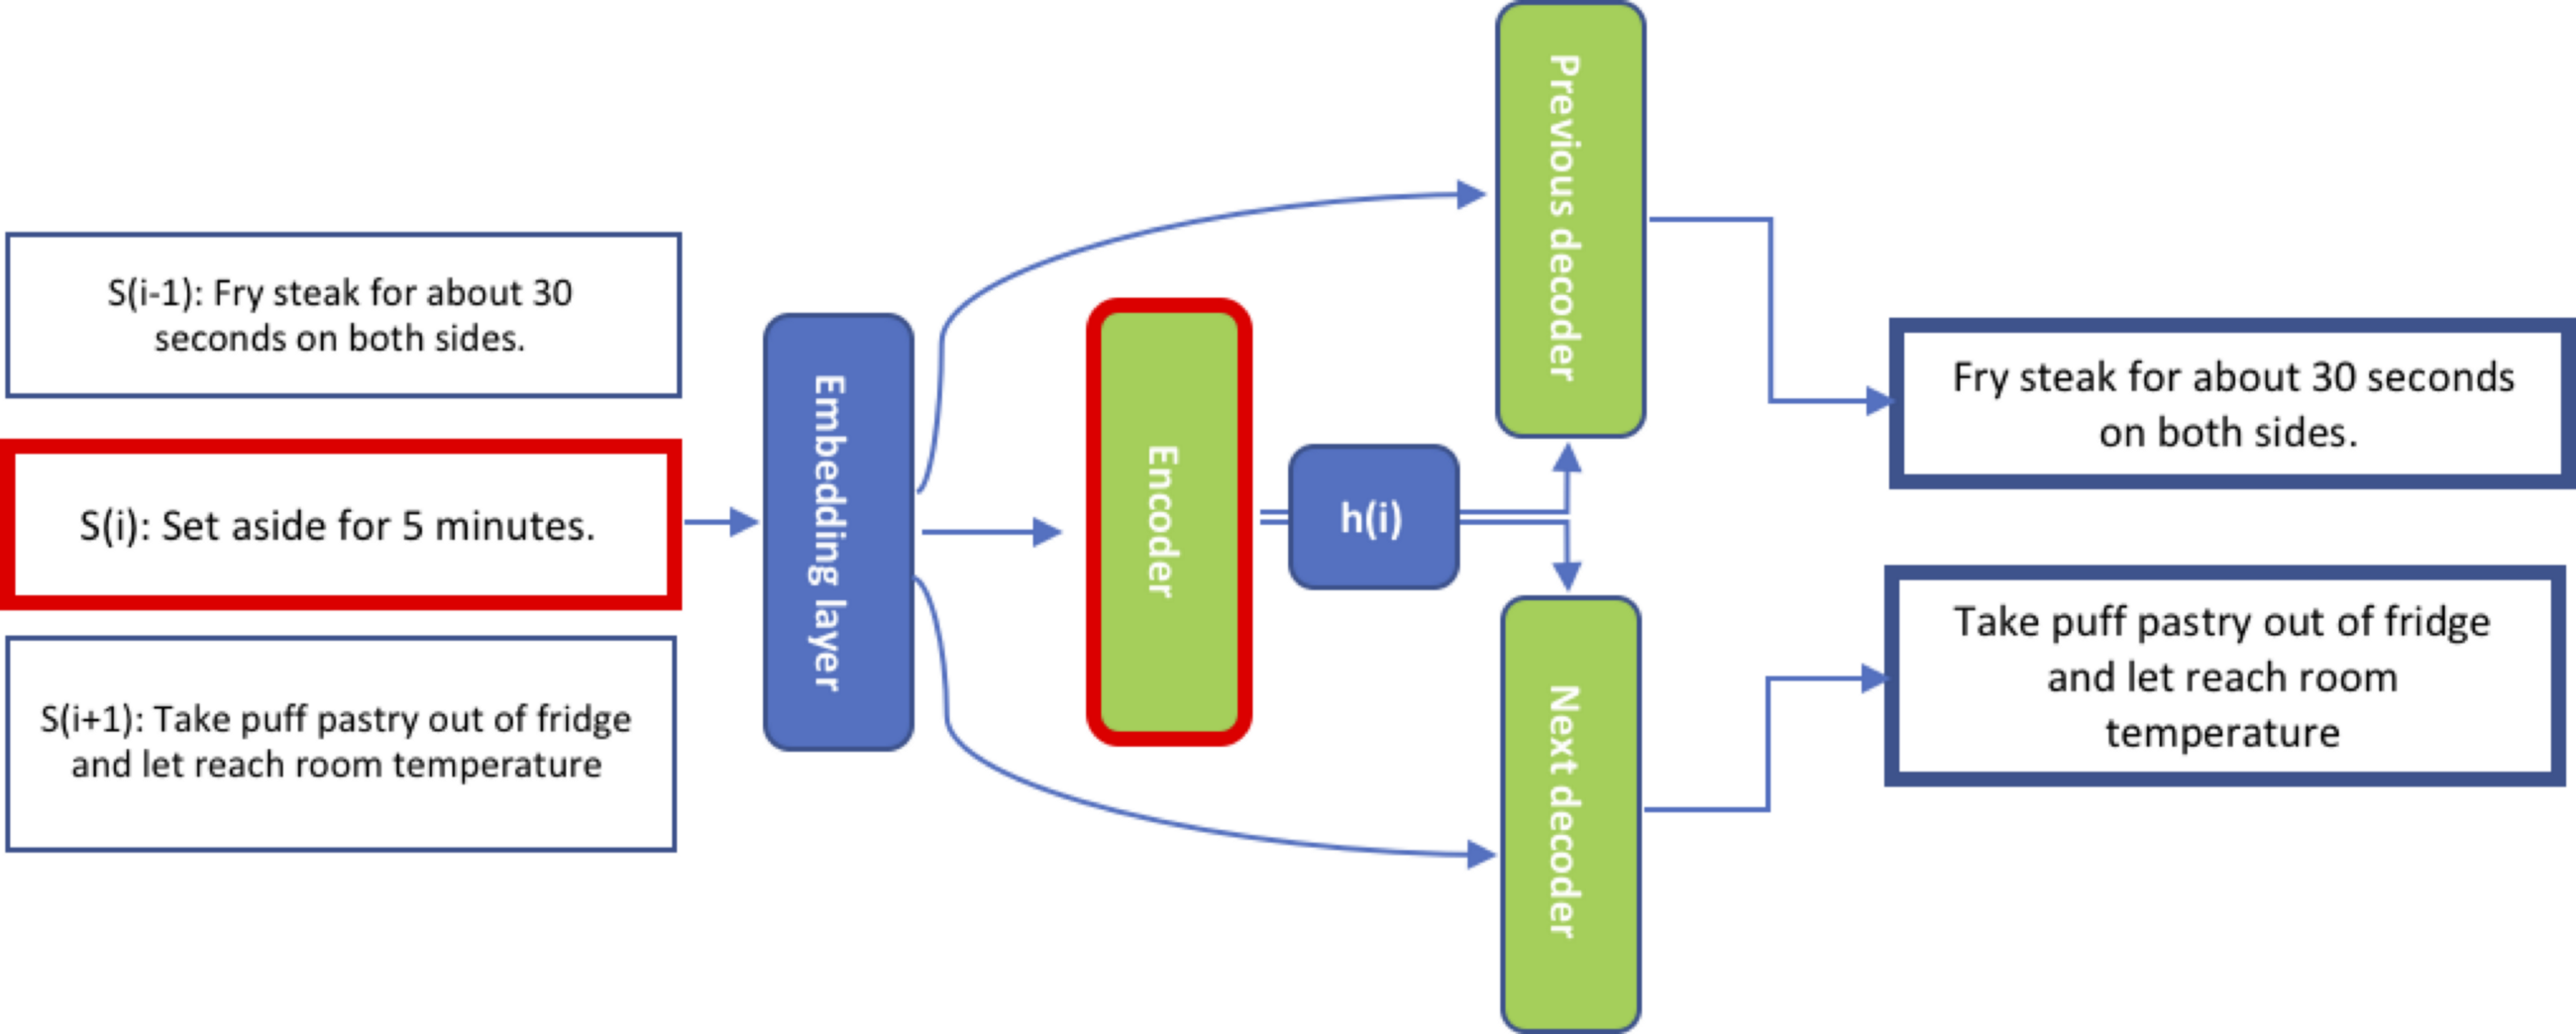
\includegraphics[width=\textwidth]{images/palachy2019/palachy2019_skip-thought.png}
	\caption[Schéma skip-thought modelu]{Schéma skip-thought modelu -- věta s(i) je zakódována enkodérem do skryté reprezentace h(i), na základě které dekodéry predikují předešlou s(i--1) a následující s(i+1) větu\cite{palachy2019}}
	\label{fig:palachy2019ST}
\end{figure}

\subsubsection*{Quick-thought vektory}
Skupina pod vedením Logenswarana\cite{logenswaran2018} navrhla přeformulováním úlohy embeddingu dokumentů zcela nový přístup. Kontext, ve kterém se věta vyskytuje, začali predikovat metodou učením s učitelem. Viz. obrázek \ref{fig:palachy2019QT}.
\begin{figure}\centering
	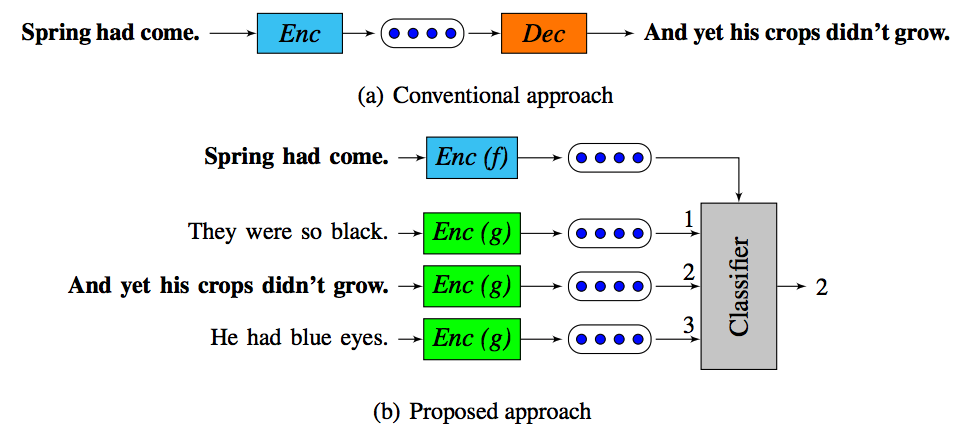
\includegraphics[width=0.9\textwidth]{images/palachy2019/palachy2019_QT.png}
	\caption{Schéma modelu quick-thought (b) oproti skip-thought (a) \cite{palachy2019}}\label{fig:palachy2019QT}
\end{figure}

% \subsubsection{FastSent}
% Hill ve své práci\cite{hill2016} navrhl zjednodušené řešení skip-thought modelu, kde místo enkodéru a dvou dekodérů se používá klasický BOW. Díky tomu je dosaženo značného snížení výpočetní náročnosti.

\subsubsection*{Word Mover's Embedding}
Metoda je založená na „Word Mover’s Distance“\cite{kusner2015} -- metrice pro podobnost mezi dvěma dokumenty definováná jako minimální vzdálenost, kterou potřebují embedovaná slova jednoho dokumentu urazit ve vektorovém prostoru k dosažení embedovaných slov druhého dokumentu. K těmto účelům bylo navrženo D2KE (z angl. distances to kernel and embeddings)\cite{wu2018}, jako metodologii pro odvození kernelu z dané vzdálenostní funkce. Na obrázku \ref{fig:palachy2019WME} je zobrazeno odvození takového kernelu.
\begin{figure}\centering
	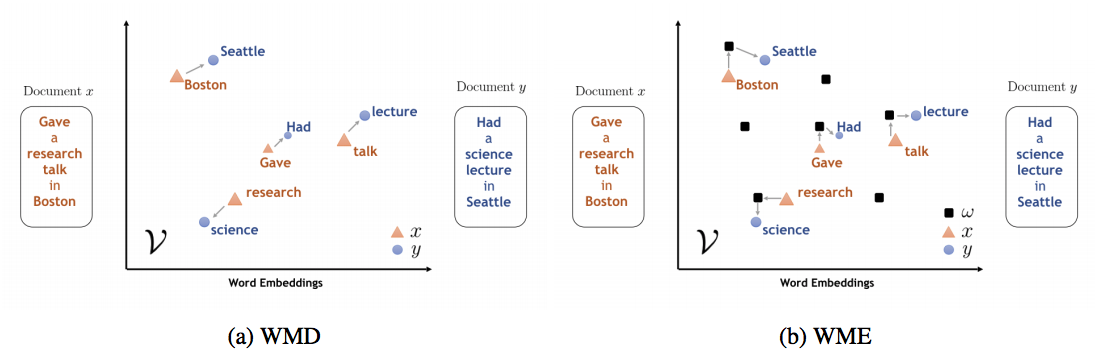
\includegraphics[width=\textwidth]{images/palachy2019/palachy2019_WME.png}
	\caption{Ukázka vztahu WMD (a) a WME (b) s kernelem odvozeným na základě množiny náhodných dokumentů\cite{palachy2019}}\label{fig:palachy2019WME}
\end{figure}

Více do detailu Palachy popisuje ve článku\cite{palachy2019}.

\subsubsection*{ULMFiT}
Zde se nejedná přímo o metodu embeddingu, jako spíš o inovativní přístup k řešení úloh zpracování přirozeného jazyka. ULMFiT (z angl. Universal Language Model Fine-tuning)\cite{hovard2018} přichází jako první s aplikací metody tzv. „transfer-learningu“ v NLP. Metoda spočívá ve třech krocích:
\begin{enumerate}
    \item Základní před-trénování jazykového modelu (například na textu z Wikipedie).
    \item Ladění (z angl. fine-tune) jazykového modelu na cílové doméně.
    \item Ladění klasifikátoru pro cílovou úlohu.
\end{enumerate}
Podle článku\cite{ghelani2019}, tímto způsobem použitá síť výrazně překonala dosavadní state-of-the-art řešení na několika úlohách klasifikace textu.

\subsubsection*{ELMo}
V práci Peters a spol\cite{peters2018} přichází s myšlenkou hluboce „kontextualizovaných“ slovních embeddingů. Místo přiřazování fixních embeddingů každému slovu, ELMo (z anlg. Embeddings from Language Model) používá oboustrannou LSTM (z angl. bi-directional long short-term memory) síť ke zpracování celé věty, čímž vytváří embedding pro slova na základě kontextu z obou stran. Vnitřní reprezentace slov je založená na jednotlivých znacích, čímž se model stává robustnějším pro slova mimo slovník použitý při trénování.

Alammar\cite{alammar2018} přehledně prezentuje celý proces ELMo embeddingu.

\subsubsection*{Transformers}
Práce „Attention Is All You Need“\cite{vaswani2017} odstartovala novou éru v oboru zpracování přirozeného jazyka. Vznikla rodina modelů typu tzv. Transformer, který se vyhýbá konvolučnímu i rekurentnímu přístupu ke zpracování sekvence a místo toho používá inovativní přístup zvaný „attention“. Stále však uchovávají architekturu enkodér (čtení vstupu) -- dekodér (provádění predikce).

Tyto modely generují kontextové embeddingy obsahující informaci o sousedních slovech, přestože jejich cílem není tvořit bohatý embedovací prostor pro vstupní text.
 Na obrázku \ref{fig:alammar2018transformer} je zobrazeno schéma enkodér--dekodér architektury Transformer.
\begin{figure}\centering
	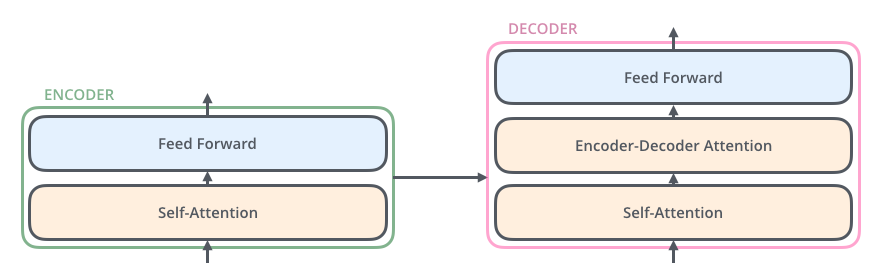
\includegraphics[width=\textwidth]{images/alammar2018_transformer.png}
	\caption{Ilustrace enkodér-dekodér architektury Transformer\cite{palachy2019}}\label{fig:alammar2018transformer}
\end{figure}

\subsubsection*{USE}
„Universal Sentence Encoder“\cite{cer2018} přichází s unikátní myšlenkou učení enkodéru pro získání embeddingů vět. USE je založený na skip-thought modelu, avšak místo obou částí enkodér--dekodér architektury je použito pouze architektury se sdíleným enkodérem, který je paralelně učený na různých úlohách. Tím autoři cílí na vytvoření jednoho univerzálního enkodéru, schopného plnit roli embedování vět v různých aplikacích jako je klasifikace, klastrování či podobnost textu.

Autoři USE přichází se dvěma možnostmi řešení enkodéru. První používá tzv. hluboce průměrovanou síť (z angl. deep averaging network), zatímco druhá se opírá o složitější strukturu transformeru\cite{yang2018}.
 Na obrázku \ref{fig:yang2018USE} je zobrazena architektura sdílení enkodéru.
\begin{figure}\centering
	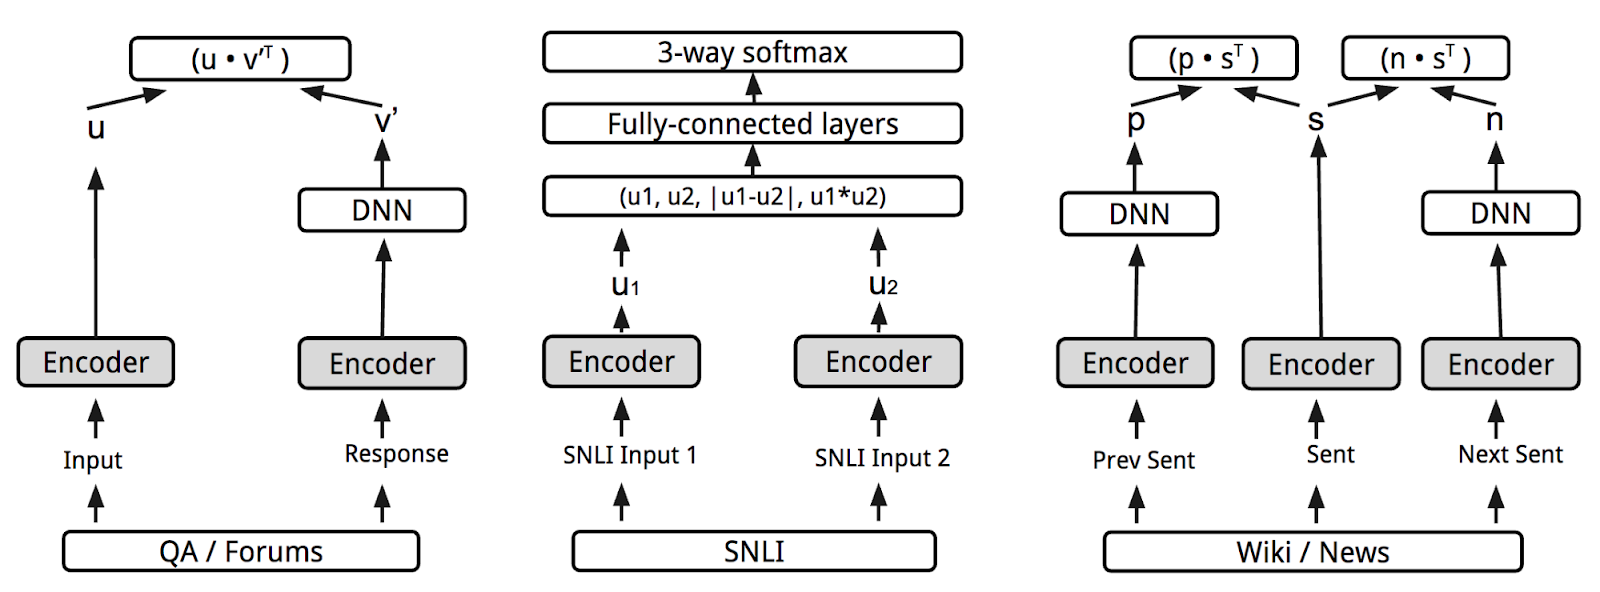
\includegraphics[width=\textwidth]{images/yang2018_USE.png}
	\caption{Architektura paraleního učení modelu USE se sdíleným enkodérem\cite{yang2018}}\label{fig:yang2018USE}
\end{figure}

\subsubsection*{GPT}
Jako jednou z prvních adaptací Transformer architektury je GPT (z angl. Generative Pre-Training Transformer)\cite{radford2018}. Oproti základní architektuře používá však jinou strukturu. GPT se skládá pouze z na sebe napojených bloků dekodéru. Vyškálováním modelu autoři později dosáhli lepšího modelu, pojmenovaného jako GPT-2\cite{radford2019}.

Ve svém článku\cite{liang2019} Liang uvádí, že GPT se řadí mezi tzv. autoregresivní jazykové modely, které používají kontextových slov k predikci slova následujícího. Přístup autoregresivních jazykových modelů je ovšem omezující na dva směry, buď dopředný, nebo zpětný, jako je zobrazeno na obrázku \ref{fig:liang2019GPT}.
\begin{figure}\centering
	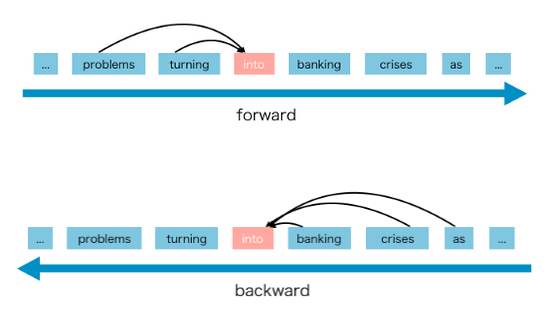
\includegraphics[width=0.8\textwidth]{images/liang2019/liang2019_GPT.png}
	\caption{Směrově orientované predikce autoregresivního jazykového modelu\cite{liang2019}}\label{fig:liang2019GPT}
\end{figure}

\newpage
\subsubsection*{BERT}
Dalším z úspěšných modelů Transformer rodiny je BERT (z angl. Bidirectional Encoder Representations from Transformers)\cite{devlin2018}, který způsobil rozruch v komunitě, kvůli dosažení state-of-the-art výsledků v mnoha různých úlohách zpracování přirozeného jazyka, říká Horev\cite{horev2018}.

BERT je navržený pro modelování jazyka a jeho následné jednoduché ladění. Díky tomu potřebuje oproti klasickému Transformer modelu pouze mechanizmus enkodéru.

Autoři modelu přišli na nový způsob řešení predikce slova na základě kontextu. BERT nepredikuje následující slovo, ale slovo zamaskované speciální značkou. Takovému přístupu se říká autoenkódovací jazykový model (z angl. autoencoder language model), viz. obrázek \ref{fig:liang2019BERT}.
\begin{figure}\centering
	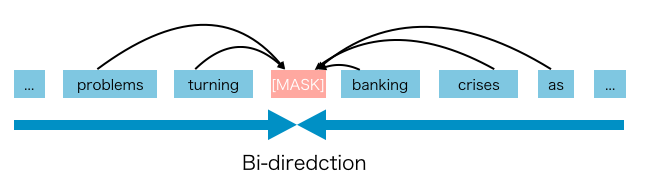
\includegraphics[width=0.8\textwidth]{images/liang2019/liang2019_BERT.png}
	\caption{Obousměrně orientovaný autoenkodér\cite{liang2019}}\label{fig:liang2019BERT}
\end{figure}
Této inovace BERT využívá pro komplexnější využití kontextové informace.

Narozdíl od autoregresivních modelů enkodér modelu BERT může číst celou sekvenci slov najednou, přestože název modelu je odvozen od dvousměrného čtení, jak je zobrazeno na obrázku \ref{fig:alammar2018BERT}.

% Mnohem více do detailu o architektuře Transformer a BERT popisuje Jay Alammar ve svých ilustrovaných článcích\cite{alammar2018}\cite{alammar2018b}.
Mnohem více do detailu je popsáno v ilustrovaných článcích\cite{alammar2018}\cite{alammar2018b}.
\begin{figure}\centering
	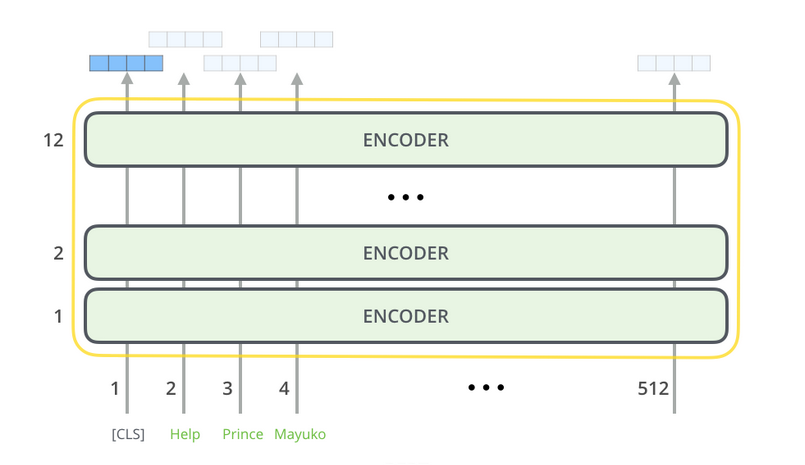
\includegraphics[width=0.8\textwidth]{images/alammar2018_BERT.png}
	\caption{Ilustrace architektury modelu BERT\cite{alammar2018}}\label{fig:alammar2018BERT}
\end{figure}

\subsubsection*{Sentence-BERT}
Jak je vidět na obrázku \ref{fig:alammar2018BERT}, BERT doplňuje sekvenci tokenů o speciální token [CLS], kde jeho výstup lze používat pro klasifikační úlohy. Autoři modelu Sentence-BERT však ukazují\cite{reimers2019}, že poskytuje pouze slabý embedding pro jiné než klasifikační úlohy. Navrhli proto architekturu využívající BERT jako základ pro tzv. „siamese“ a „triplet“(zachycené na obrázku  \ref{fig:palachy2019SBERT}) síťovou strukturu, kterou by bylo možné zachycovat sémanticky smysluplné embeddingy vět. Tím se jim podařilo překonat dosavadní state-of-the-art metody pro embedding vět.
\begin{figure}\centering
	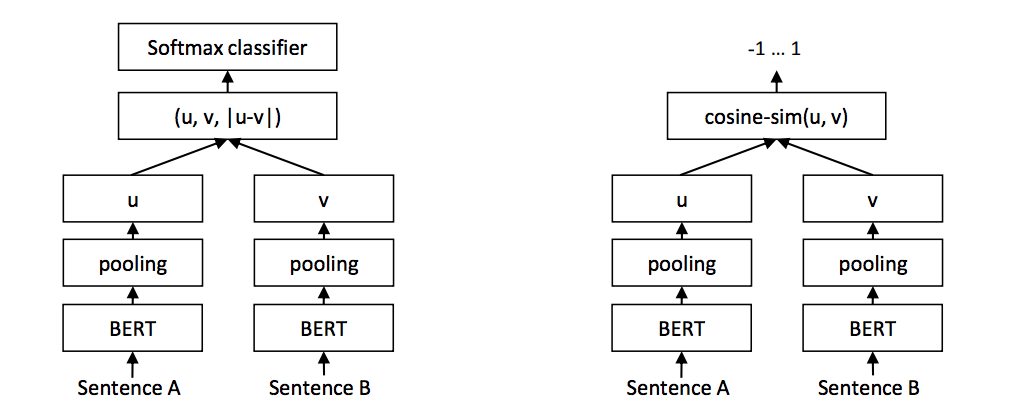
\includegraphics[width=\textwidth]{images/palachy2019/palachy2019_SBERT.png}
	\caption{Architektura SBERT pro trénování klasifikátoru a počítání kosinové podobnosti\cite{palachy2019}}\label{fig:palachy2019SBERT}
\end{figure}

\subsubsection*{XLNet}
XLNet\cite{yang2019} je model odvozený od modelu Transformer-XL\cite{dai2019}, který vznikl jako rozšíření klasického transformeru ve smyslu zrušení omezení vstupu fixní délky. Jak Liang vysvětluje ve svém článku\cite{liang2019}, princip autoenkodéru v modelu BERT přinesl i svá omezení. Proto autoři modelu XLNet navrhli tzv. permutační modelování jazyku (z angl. permutation language modeling). To umožňuje modelu využít kontextu z obou stran, přestože zůstává být autoregresivní, jak je naznačeno na obrázku \ref{fig:palachy2019SBERT}. Tyto inovace se opět projevily pozitivně na vlastnosti modelu, díky čemu zaujal state-of-the-art výsledky pro mnoho NLP úloh.
\begin{figure}\centering
	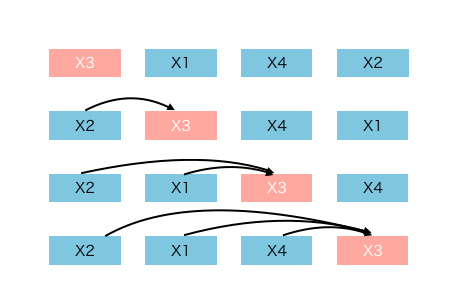
\includegraphics[width=0.5\textwidth]{images/liang2019/liang2019_XLNet.png}
	\caption{Permutační modelování jazyka\cite{liang2019}}\label{fig:liang2019XLNet}
\end{figure}

\subsubsection*{Další}
Vývoj jazykových modelů je stále v rozmachu a tak skoro každý měsíc vychází publikace s nějakým novým objevem. V mé práci nemůžu ani zdaleka obsáhnout vše zajímavé, nicméně jeden z velice vyčerpávajících a aktuálních přehledů je například ve článku\cite{suryavansh2020} od Manua Suryavanshe.

\subsubsection{Metody učení s učitelem}
Palachy ve svém článku\cite{palachy2019} dále uvádí několik přístupů řešení embeddingu pomocí metod učení s učitelem. Pro účely mé práce tyto metody však nejsou důležité, proto je konkrétně nezmiňuji.

\newpage
\subsection{Výběr metody a technologie}
Pro výběr vhodného modelu pro aplikaci při vyhodnocování podobnosti textů stanovuji tato kritéria. Vzhledem k doméně mé práce -- české veřejné zakázky -- potřebuji, aby byl model schopný pracovat s českým jazykem. Zároveň však nedisponuji prostředky k učení modelu na českém korpusu od nuly, tedy potřebuji najít před-trénovaný model podporující češtinu. Kandidátní modely poté experimentálně vyhodnocuji k finálnímu výběru toho nejvhodnějšího.

\subsubsection{Dostupné před-trénované modely}
Naprostá většina různých modelů je poskytována pouze s anglickými před-trénovanými modely, kvůli čemu se pro mé účely stávají nevhodnými.

% Dle dosavadních state-of-the-art výsledků podle portálu paperswithcode.com v kategorii sémantické podobnosti textů se nejlépe umísťují modely XLNet a ALBERT\cite{lan2019}. Ani pro jeden z těchto modelů není publikovaný před-trénovaný model s podporou češtiny, viz. repozitář \textit{zihangdai/xlnet}\footnote{XLNet repozitář -- https://github.com/zihangdai/xlnet} a web \textit{Huggingface Transformers}\footnote{Huggingface Transformers web -- https://huggingface.co/transformers/pretrained\_models.html}. 
Dosavadní state-of-the-art výsledky podle portálu paperswithcode.com v kategorii sémantické podobnosti textů ukazují, že nejlépe se umísťují modely XLNet a ALBERT\cite{lan2019}. Ani pro jeden z těchto modelů není publikovaný před-trénovaný model s podporou češtiny, viz. repozitář \textit{zihangdai/xlnet}\footnote{XLNet repozitář -- https://github.com/zihangdai/xlnet} a web \textit{Huggingface Transformers}\footnote{Huggingface Transformers web -- https://huggingface.co/transformers/pretrained\_models.html}. 

Dalším nadějným kandidátem je model Sentence-BERT, který sice poskytuje vícejazyčný model \textit{distiluse-base-multilingual-cased}, avšak mezi podporovanými jazyky tohoto modelu se čeština nedostala. Model je dostupný v repozitáři autorů (\textit{UKPLab/sentence-transformers}\footnote{Sentence-BERT repozitář --  https://github.com/UKPLab/sentence-transformers}).

Model BERT se s jeho různými mutacemi dnes těší asi největší popularitě ze všech dostupných modelů. Díky tomu je také dostupné veliké množství jeho před-trénovaných modelů. Se zaměřením na češtinu jsou dostupné modely \textit{bert-base-multilingual-cased} (z oficiálního repozitáře\footnote{BERT repozitář -- https://github.com/google-research/bert/blob/master/multilingual.md} autorů) či \textit{Slavic BERT} (od skupiny \textit{DeepPavlov}\footnote{DeppPavlov web -- http://docs.deeppavlov.ai/en/master/features/pretrained\_vectors.html}).

Model USE disponuje vícejazyčnou verzí MUSE, publikovanou v práci „Multilingual Universal Sentence Encoder for Semantic Retrieval“\cite{yang2019b}. Podporuje tak 16 různých jazyků, mezi kterými však čeština není.

ULMFiT se dočkal své vícejazyčné verze MultiFiT, publikované v práci\cite{eisenschlos2019}, se kterým překonávají výsledky vícejazyčného modelu BERT. Podporuje ale jen 7 jazyků, mezi které se čeština opět nedostala.

Oproti tomu, model ELMo je vydaný s širokou podporou mnoha jazyků pod repozitářem \textit{HIT-SCIR/ELMoForManyLangs}\footnote{ElMoForManyLangs repozitář - https://github.com/HIT-SCIR/ELMoForManyLangs}. Mimo jiné tak pro model ELMo existuje i česká verze.

Dalším široce rozšířeným modelem je fastText, který nabízí různé před-trénované modely pro až 157 jazyků. Všechny modely včetně českého jsou dostupné na webu \textit{fasttext.cc}\footnote{FastText web - https://fasttext.cc/docs/en/crawl-vectors.html}

% Ostatní modely jako GPT, Sent2vec, FastSent či GloVe před-trénované modely buď vůbec nemají, nebo mají jen pro anglický jazyk. Jedině pro model GloVe existuje vícejazyčné rozšíření (dostupné na webu \textit{GloVe}\footnote{GloVe web - http://www.cs.cmu.edu/~afm/projects/multilingual\_embeddings.html}), které ovšem podporu češtiny také neposkytuje.
Ostatní modely jako GPT, Sent2vec či GloVe před-trénované modely buď vůbec nemají, nebo mají jen pro anglický jazyk. Jedině pro model GloVe existuje vícejazyčné rozšíření (dostupné na webu \textit{GloVe}\footnote{GloVe web - http://www.cs.cmu.edu/~afm/projects/multilingual\_embeddings.html}), které ovšem podporu češtiny také neposkytuje.

\subsection{Vyhodnocení modelů}
\label{sec:model_evaluation}
Zatímco na anglický jazyk se zaměřuje po celém světě mnoho lidí, pro vyhodnocení metod embeddingů pro češtinu zatím vzniklo jen pár prací.

Jednou z nich je práce Karolíny Hořeňovské -- „An evaluation of Czech word embeddings“\cite{horenovska2019}, kde autorka zmiňuje, že pro češtinu se mohou modely výkonnostně lišit od výsledků pro angličtinu. Uvádí to na příkladu CBOW architektury, která pro češtinu funguje lépe než skip-gram, zatímco pro angličtinu je to naopak. Navíc se v tom shoduje s předešlou prací „New word analogy corpus for exploring  embeddings  of Czech words“\cite{svoboda2016}. Stejně tak se shodují v tom, že GloVe model pro češtinu nefunguje dobře. Dále Hořeňovská uvádí, že i model BERT pro podobnost českých textů dosahuje překvapivě slabých výsledků.

Nejlépe se jeví model fastText, který na datasetu „Czech Dataset for Semantic Similarity and Relatedness“\cite{konopik2017} dosahuje z testovaných modelů nejlepších výsledků.

Jedním z metodik pro vyhodnocování jazykových modelů je úloha STS (z angl. Semantic Textual Similarity), která se stala hlavní úlohou tzv. SemEval (International Workshop on Semantic Evaluation). STS úloha znamená ohodnocování podobnosti dvou textových fragmentů, přičemž výsledky STS systémů jsou porovnávány s manuálně anotovanými daty. Toto porovnávání se typicky měří korelací.

V základu jsou datasety pro STS úlohu anglické, ale v práci „Czech Dataset for Semantic Textual Similarity“\cite{svoboda2018} publikují českou verzi, jako překlad původního anglického datasetu. Dataset je dostupný v repozitáři \textit{Svobikl/sts-czech}\footnote{STS Czech repozitář - https://github.com/Svobikl/sts-czech}.

V rámci práce\cite{conneau2018} vznikl nástroj pro ohodnocování kvality univerzálních reprezentací vět, tzv. \textit{SentEval}. Tento nástroj obsahuje, mimo jiné, i úlohy STS. Své experimentální vyhodnocení modelů pro embedding textu tak zakládám na tomto nástroji, který dále upravuji pro použití českého STS datasetu.

Nástroj \textit{SentEval} je dostupný ke stažení v repozitáři  \textit{facebookresearch/SentEval}\footnote{SentEval repozitář - https://github.com/facebookresearch/SentEval}. V základní verzi nepodporuje vyhodnocení embeddingů pro delší úseky textu (například celé věty), ale pouze po jednotlivých tokenech (slovech), které pouze agreguje pro získání embeddingu celého fragmentu. Dnešní modely ovšem dokážou provádět embedding pro celé věty, a proto nástroj upravuji, abych byl pomocí něj schopný vyhodnocovat embeddingy celých vět.

Vzdálenost mezi embeddingy dvou textových fragmentů každého vzorku je měřena kosinovou vzdáleností. Jako výsledek \textit{SentEval} vrací Pearsonovy a Spearmanovy korelační koeficienty mezi podobností vypočítanou z embeddingů a manuálně anotovanou.

Pro experimentální vyhodnocení vybírám několik následujících modelů:
\begin{itemize}
    \item \textit{bert-base-multilingual-cased}\\
    Vícejazyčný model typu BERT, nativně používaný NLP frameworkem \textit{Transformers} (\textit{huggingface/transformers}\footnote{Transformers repozitář - https://github.com/huggingface/transformers})
    \item \textit{multi\_cased\_L-12\_H-768\_A-12}\\
    Vícejazyčný model typu BERT, dostupný z oficiálního repozitáře \textit{google-research/bert}\footnote{BERT repozitář - https://github.com/google-research/bert/blob/master/multilingual.md}, ve formě tensorflow model checkpointu
    \item \textit{bg\_cs\_pl\_ru\_cased\_L-12\_H-768\_A-12\_v1}\\
    Vícejazyčný (podporující bulharštinu, češtinu, polštinu a ruštinu) model typu BERT, dostupný z webu NLP frameworku \textit{deeppavlov}\footnote{DeppPavlov web - http://docs.deeppavlov.ai/en/master/features/models/bert.html}, ve formě tensorflow model checkpointu
    \item \textit{bert-base-cased}\\
    Anglický model typu BERT, nativně používaný NLP frameworkem \textit{Transformers} (\textit{huggingface/transformers})
    \item \textit{cc\_cs\_300\_fasttext}\\
    Český model typu fastText, dostupný z webu frameworku \textit{fastText}, v binární formě používané knihovnou \textit{fasttext}
    \item \textit{cc\_en\_300\_fasttext}\\
    Anglický model typu fastText, dostupný z webu frameworku \textit{fastText}, v binární formě používané knihovnou \textit{fasttext}
    \item \textit{wiki\_cs\_300\_fasttext}\\
    Český model typu fastText, dostupný z webu frameworku \textit{fastText}, v binární formě používané knihovnou \textit{fasttext}, trénovaný na Wikipedii
    \item \textit{elmo\_139}\\
    % Český model typu ELMo, dostupný z repozitáře \textit{HIT-SCIR/ELMoForManyLangs}, ve formě používané framewokem \textit{elmoformanylangs}
    Český model typu ELMo, dostupný z repozitáře \textit{ELMoForManyLangs}, ve formě používané framewokem \textit{elmoformanylangs}
\end{itemize}

Dále na jednotlivých modelech provádím různé modifikace podle toho, co umožňují frameworky s nimi pracující.

Pro modely BERT, které vrací pro každý text množinu vektorů, tak v základní verzi vybírám pouze první z nich (dříve zmiňovaný [CLS] vektor), zatímco ve verzi s příponou \textit{mean\_pooled}(viz. následující tabulky) používám všechny vektory sloučené tzv. \uv{mean poolingem} po složkách.

Vedle toho, knihovna \textit{fasttext} umožňuje dvojí přístup k získání embeddingu, kde oba vrací odlišné vektory. První je embedding pro slovo (přípona \textit{word}) a druhý pro celé věty (přípona \textit{sentence})

Při vyhodnocování provádím 4 různé testy jak pro český, tak anglický dataset a oběma přístupy vyhodnocování embeddingů podle jednotlivých tokenů (základní přístup) i celých vět (upravený přístup):

\begin{itemize}
    \item \textit{STSCZ}\\
    STS úloha na českém datasetu prováděná základním přístupem nástroje \textit{SentEval}, viz. tabulka \ref{table:STSCZ}
    \item \textit{STSCZ2}\\
    STS úloha na českém datasetu prováděná upraveným přístupem pro vyhodnocení embeddingů celých vět , viz. tabulka \ref{table:STSCZ2}
    \item \textit{STS16}\\
    STS úloha na oficiálním anglickém datasetu STS16 prováděná základním přístupem nástroje \textit{SentEval}, viz. tabulka \ref{table:STS16}
    \item \textit{STS162}\\
    STS úloha na oficiálním anglickém datasetu STS16 prováděná upraveným přístupem pro vyhodnocení embeddingů celých vět, viz. tabulka \ref{table:STS162}
\end{itemize}

Výsledky experimentů jsou zobrazené v tabulkách níže.

\begin{table}[h!]
\centering
\begin{tabular}{ |l|c|c| }
 \hline
 \multicolumn{3}{|c|}{\textit{STSCZ}} \\\hline
 \hline
  Název modelu & Pearson & Spearman \\\hline
\textit{wiki\_cs\_300\_fasttext\_sentence} & 0.634602 &	0.645182\\
\textit{wiki\_cs\_300\_fasttext\_word} & 0.619290 & 0.625226\\
\textit{cc\_cs\_300\_fasttext\_sentence} & 0.616563 & 0.624195\\
\textit{multi\_cased\_L-12\_H-768\_A-12\_mean\_pooled} & 0.536009 & 0.589423\\\hline
\textit{multi\_cased\_L-12\_H-768\_A-12} & 0.522020 & 0.576311\\
\textit{bg\_cs\_pl\_ru\_cased\_L-12\_H-768\_A-12\_v1} & 0.520884 & 0.571077\\
\textit{multi\_cased\_L-12\_H-768\_A-12\_mean\_pooled} & 0.518153 & 0.566517\\
\textit{elmo\_139} & 0.513847 & 0.531696\\\hline
\textit{bg\_cs\_pl\_ru\_cased\_L-12\_H-768\_A-12\_v1\_mean\_pooled} & 0.496374 & 0.553772\\
\textit{cc\_cs\_300\_fasttext\_word} & 0.467745 & 0.486335\\
\textit{bert-base-multilingual-cased} & 0.424912 & 0.502240\\\hline
\end{tabular}
\caption{Tabulka výsledků testu \textit{STSCZ}}
\label{table:STSCZ}
\end{table}

\begin{table}[h!]
\centering
\begin{tabular}{ |l|c|c| }
 \hline
 \multicolumn{3}{|c|}{\textit{STSCZ2}} \\\hline
 \hline
  Název modelu & Pearson & Spearman \\\hline
\textit{wiki\_cs\_300\_fasttext\_sentence} & 0.634602 & 0.645156\\
\textit{cc\_cs\_300\_fasttext\_sentence} & 0.616563 & 0.624252\\
\textit{wiki\_cs\_300\_fasttext\_word} & 0.613073 & 0.618057\\
\textit{multi\_cased\_L-12\_H-768\_A-12\_mean\_pooled} & 0.599592 & 0.612282\\\hline
\textit{multi\_cased\_L-12\_H-768\_A-12} & 0.589300 & 0.605837\\
\textit{bg\_cs\_pl\_ru\_cased\_L-12\_H-768\_A-12\_v1} & 0.557063 & 0.577191\\
\textit{cc\_cs\_300\_fasttext\_word} & 0.556476 & 0.572473\\
\textit{multi\_cased\_L-12\_H-768\_A-12\_mean\_pooled} & 0.556184 & 0.573161\\\hline
\textit{bg\_cs\_pl\_ru\_cased\_L-12\_H-768\_A-12\_v1\_mean\_pooled} & 0.536216 & 0.556067\\
\textit{bert-base-multilingual-cased} & 0.377873 & 0.425252\\
\textit{elmo\_139} & 0.335470 & 0.347201\\\hline
\end{tabular}
\caption{Tabulka výsledků testu \textit{STSCZ2}}
\label{table:STSCZ2}
\end{table}

\begin{table}[h!]
\centering
\begin{tabular}{ |l|c|c| }
 \hline
 \multicolumn{3}{|c|}{\textit{STS16}} \\\hline
 \hline
  Název modelu & Pearson & Spearman \\\hline
\textit{cc\_en\_300\_fasttext\_sentence} & 0.493155 & 0.542878\\
\textit{wiki\_cs\_300\_fasttext\_word} & 0.421575 & 0.486014\\
\textit{wiki\_cs\_300\_fasttext\_sentence} & 0.414491 & 0.481977\\
\textit{bert-base-cased} & 0.413597 & 0.527323\\
\textit{bert-base-cased\_mean\_pooled} & 0.401948 & 0.512354\\
\textit{cc\_en\_300\_fasttext\_word} & 0.273957 & 0.345844\\\hline
\end{tabular}
\caption{Tabulka výsledků testu \textit{STS16}}
\label{table:STS16}
\end{table}

\begin{table}[h!]
\centering
\begin{tabular}{ |l|c|c| }
 \hline
 \multicolumn{3}{|c|}{\textit{STS162}} \\\hline
 \hline
  Název modelu & Pearson & Spearman \\\hline
\textit{bert-base-cased\_mean\_pooled} & 0.645878 & 0.655573\\
\textit{wiki\_cs\_300\_fasttext\_word} & 0.563231 & 0.590259\\
\textit{cc\_en\_300\_fasttext\_sentence} & 0.493155 & 0.542878\\
\textit{cc\_en\_300\_fasttext\_word} & 0.484478 & 0.498747\\
\textit{bert-base-cased} & 0.461828 & 0.498818\\
\textit{wiki\_cs\_300\_fasttext\_sentence} & 0.414491 & 0.481977\\\hline
\end{tabular}
\caption{Tabulka výsledků testu \textit{STS162}}
\label{table:STS162}
\end{table}

Na výsledcích je možné pozorovat hned několik zjištění.

Zaprvé, nejdůležitější zjištění je, že nejlépe si vede model fastText, což mimo jiné potvrzuje i tvrzení v práci Hořeňovské\cite{horenovska2019}, zmíněného výše. Stejně tak se ukázalo, že model ELMo dosahuje obecně slabších výsledků. Nakonec model BERT dosahuje různých výsledků, závisejících na nastavení úlohy a volby konkrétního testu.

Zarážející zjištění je, že výsledky modelů \textit{bert-base-multilingual-cased} a \textit{multi\_cased\_L-12\_H-768\_A-12} se liší, přestože by měli být modely totožné, pouze použité jiným způsobem. Vysvětluji si to možným zveřejněním jiných verzí těchto modelů pro stažení oproti nativnímu použití frameworkem.

Stejně tak je zvláštní, že český model fastText je schopný dosahovat srovnatelných a dokonce i lepších výsledků na anglickém testu než samotné anglické modely BERT i fastText.

Změna přístupu určování embeddingu se projevila pro různé modely také různě. Zatímco u modelu fastText se téměř neprojevily, model ELMo ztratil na výkonu při embedování celé věty a model BERT zaznamenal pro některá nastavení zlepšení, ale pro některá zase zhoršení.


\subsection{Sestavení komponenty pro extrakci embeddingu}
\label{sec:component_embedding}

Komponenta pro extrakci embeddingu z textu je velice jednoduchá. Přímo využívá knihovny \textit{fasttext} pro provádění embeddingu za použití FastText modelu --- konkrétně \textit{cc\_en\_300\_fasttext\_sentence} --- který se jeví podle vyhodnocení z kapitoly \ref{sec:model_evaluation} nejlépe.

Komponenta přijímá token v podobě textového řetězce a vrací jeho embedding jako vektor reálných čísel o dimenzi 300 (defaultní nastavení modelu) v podobě \textit{numpy}\footnote{NumPy -- Python knihovna pro vědecké výpočty;\newline
dostupná z https://pypi.org/project/numpy/} pole.

Implementace komponenty je adaptovaná pro příjem kolekce tokenů, kdy vrací kolekci obsahující embedding pro každý z tokenů.

Pro inicializaci vyžaduje předání binárního \textit{fasttext} modelu, nebo alespoň systémové cesty k němu.

\newpage
\section{Extrakce předmětu}
\label{sec:subjextraction}

V této kapitole popisuji proces extrakce předmětu z dokumentace veřejných zakázek (viz. kapitola \ref{data&domain_dokumenty_vz}).

Extrakce předmětu ve své podstatě zastává stěžejní část předzpracování dat celého systému. Jejím cílem je vyextrahovat předmětnou informaci z nestrukturovaného textu celé dokumentace VZ. Přestože jsou data dokumentace VZ nestrukturovaná, jde o poměrně specifický typ dat, ve kterém se zpravidla opakují určité vzorce. Tento proces se snaží využít těchto vzorců k předzpracování textu, primárně spočívajícího v čistění dat v podobě různého filtrování, transformací a extrakcí.

\subsection{Návrh procesu extrakce předmětu}
\label{sec:subj_extraction_design}

Při tvz. \uv{black-box} pohledu na proces je na vstupu veškerá dostupná dokumentace veřejné zakázky a na výstupu výčet konkrétních předmětných částí této VZ.

Pro takovou transformaci navrhuji proces sestávající z těchto hlavních kroků (podprocesů):
\begin{enumerate}
    \item Extrakce textu z dokumentů
    \item Identifikace kontextu předmětu v dokumentech
    \item Filtrování a transformace kontextu
    \item Extrakce předmětných částí podle lokálních charakteristik
    \item Extrakce předmětných částí podle větného rozkladu
\end{enumerate}

\begin{quote}
    V textu dále používám specifické názvosloví pro symbolické odlišení druhu procesů, které provádí operace s částmi textu:
    \begin{itemize}
        \item filter:= odfiltrovává; část textu, která vyhovuje podmínce, je odstraněna,
        \item transformer:= transformuje; část textu, která vyhovuje podmínce, je nahrazena definovanou či odvozenou náhradou,
        \item extraktor:= extrahuje; část textu, která vyhovuje podmínce, je ponechána.
    \end{itemize}
\end{quote}

Celý proces je schématicky znázorněn na obrázku \ref{fig:subjextraction}.
\begin{figure}\centering
	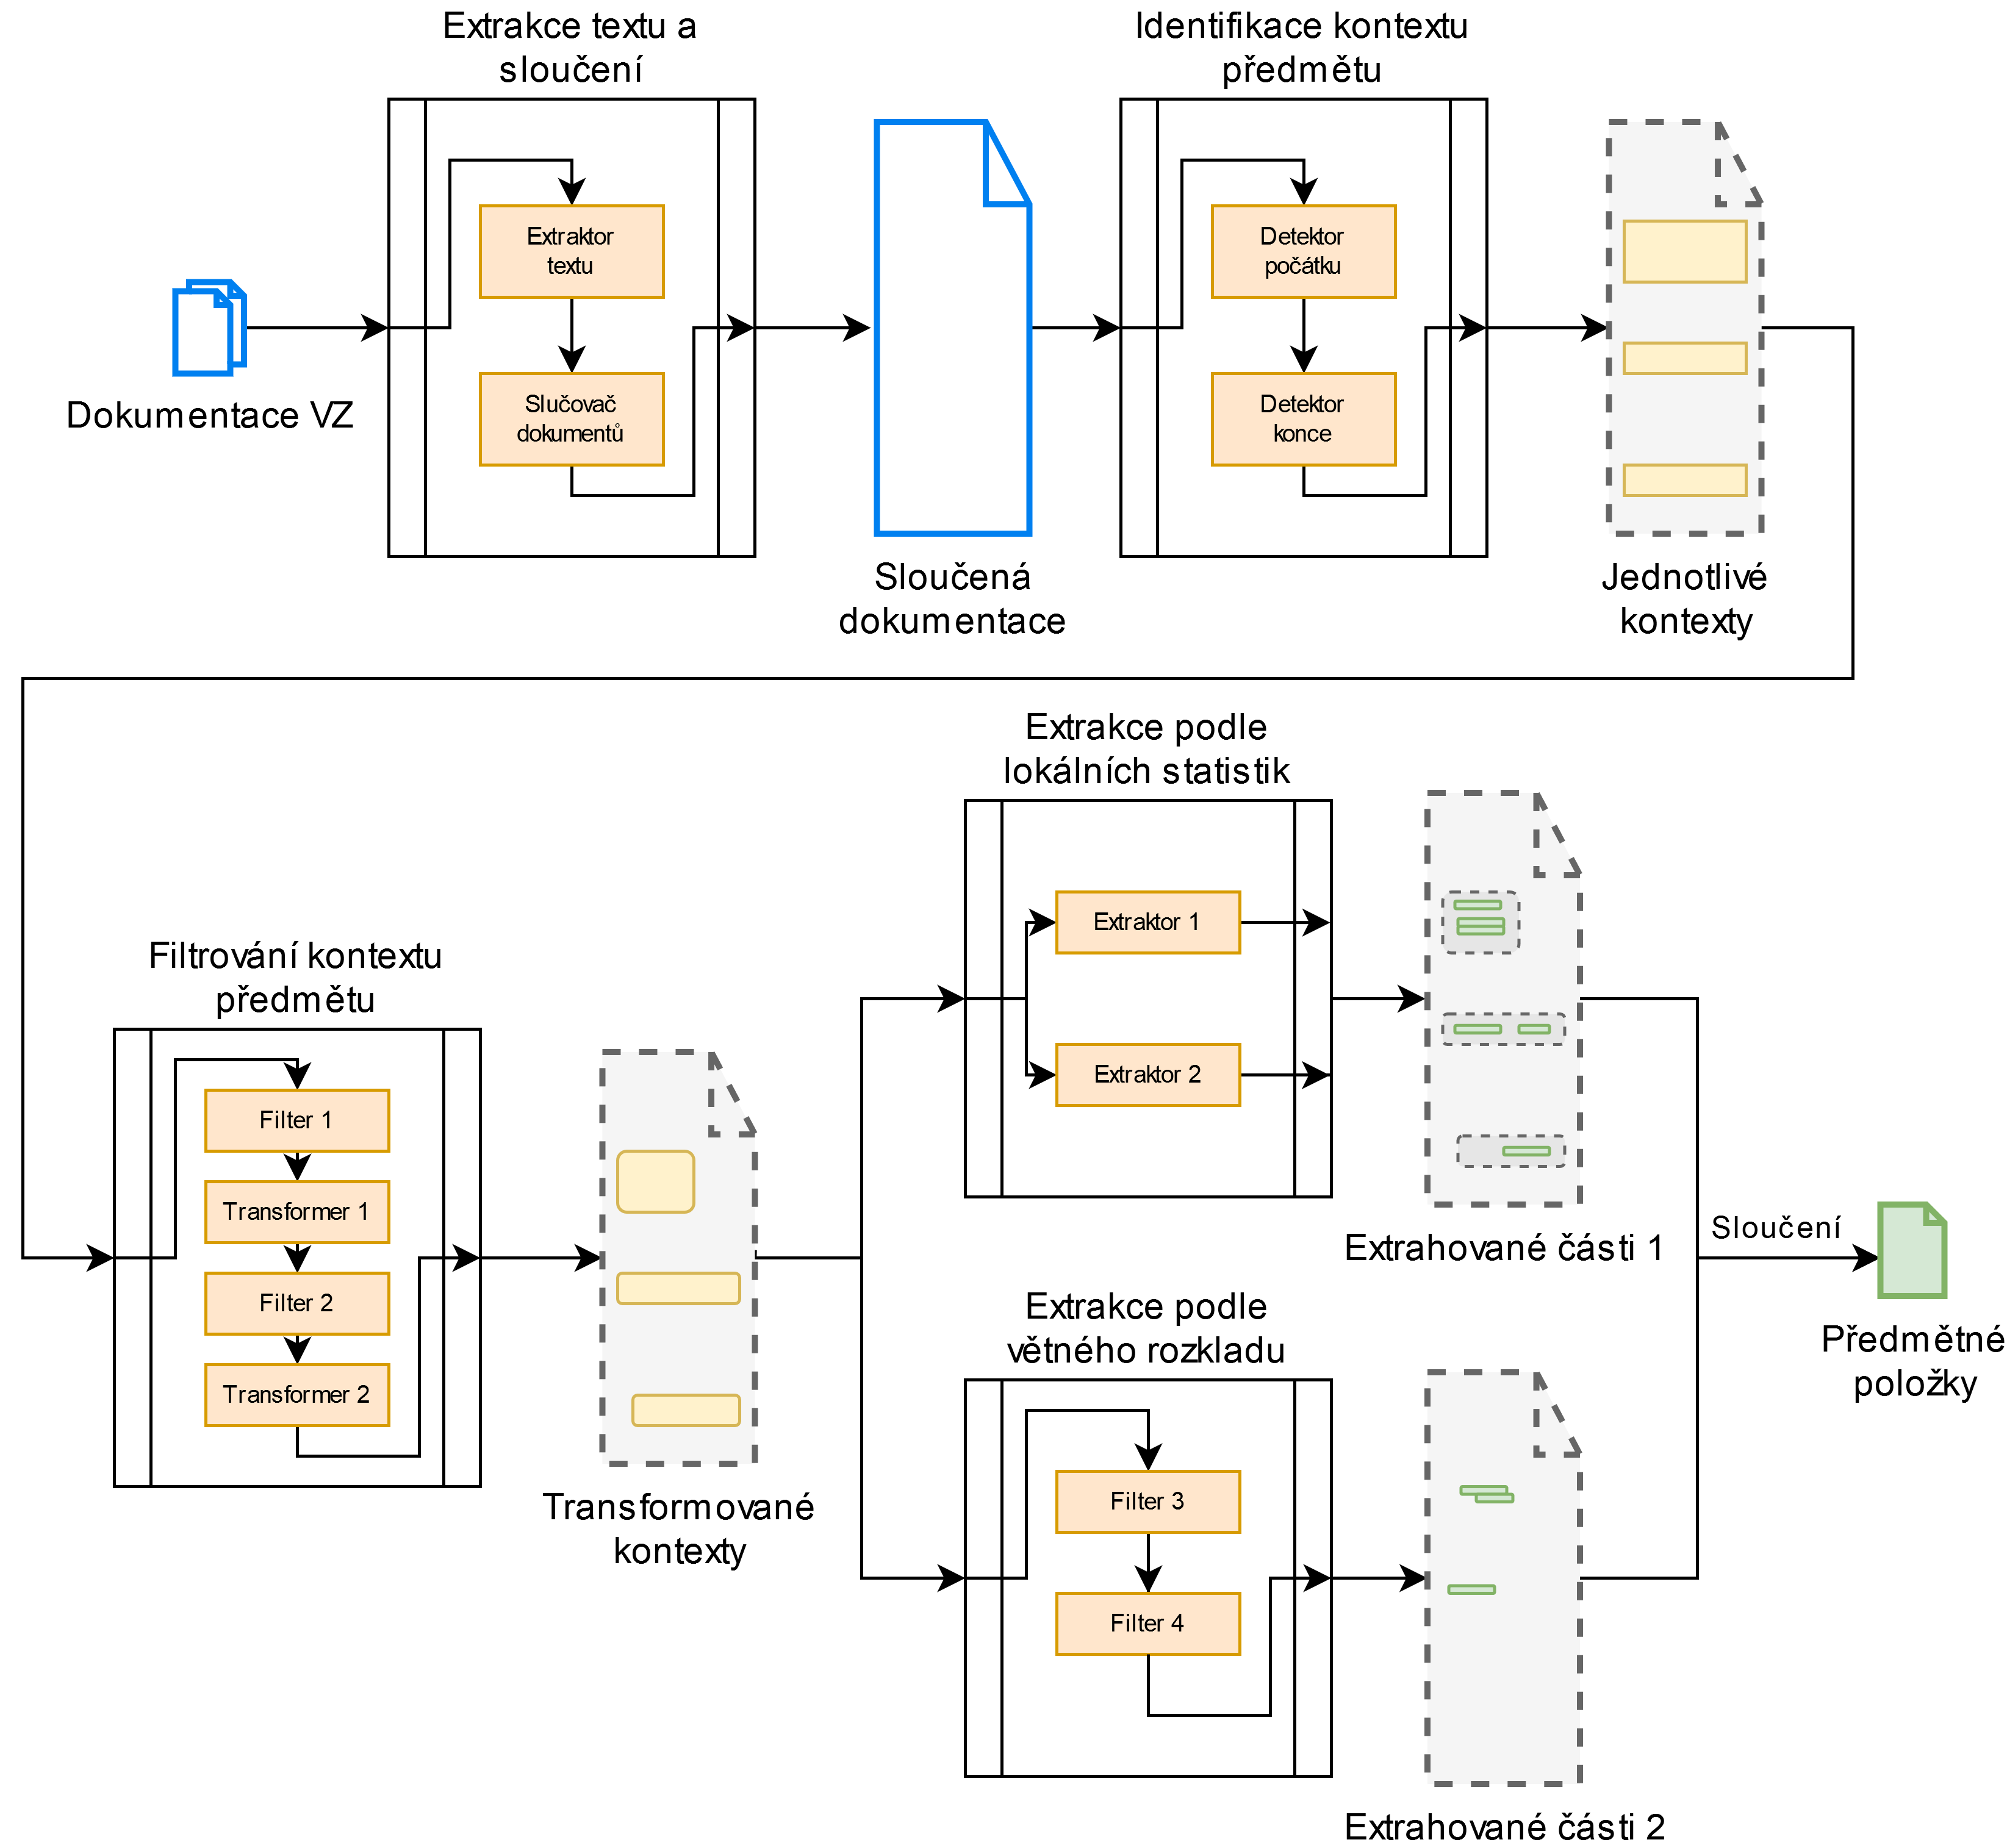
\includegraphics[width=1\textwidth]{images/subj_extraction.png}
	\caption{Schéma procesu extrakce předmětu dokumentace VZ}\label{fig:subjextraction}
\end{figure}


\subsection{Extrakce textu z dokumentů}
Jak napovídá schéma \ref{fig:subjextraction}, na vstupu procesu extrakce textu je veškerá dostupná dokumentace k VZ v podobě tzv. \uv{formátovaného} textu (z angl. rich-text). Na výstupu se poté očekává souvislý \uv{prostý} text (z angl. plain-text).

V dokumentaci VZ se standarně vyskytují předsmluvní dokumenty, přílohy (projektové dokumentace, specifikace), smlouvy a mnoho dalšího. Z většiny se jedná o textové dokumenty ve formátu \textit{.pdf} či \textit{.doc/.odt}, ale vyskytují se i~další od tabulek (\textit{.xls}), přes obrázky (\textit{.jpg}) až po komplexní archivy (\textit{.zip}) nebo certifikáty (\textit{.cer}). Ze všech těchto formátů potřebuji extrahovat prostý text.

K tomu využívám nástroje projektu \textit{public-contracts}, který je jako open-source dostupný v repozitáři \textit{opendatalabcz/public-contracts}\footnote{opendatalabcz/public-contracts repozitář\newline --
dostupný z https://github.com/opendatalabcz/public-contracts},
vyvíjeného v rámci laboratoře otevřených dat
\textit{OpenDataLab}\footnote{OpenDataLab web -- dostupný z https://opendatalab.cz/}, který používá pro extrakci textu nástroje \textit{Apache Tika} s OCR technologií \textit{Tesseract}.

Samotný projekt \textit{public-contracts} řeší vyhledávání českých VZ, stejně jako stahování jejich dokumentace, extrakci textu z nich a následné uložení do databáze. Implementován je v jazyku Java a pro ukládání vyextrahovaných textů používá databázi Postgres.

Takto vyextrahovaný text nakonec slučuji pro použití v dalším procesu.

\subsection{Identifikace kontextu předmětu}
\label{sec:subj_context_identification}

Některé zakázky obsahují rozsáhlé projektové dokumentace o desítkách až stovkách stran. Kvůli tomu je nutné takový rozsah omezit na kontext, ve kterém se pojednává o samotném předmětu. Zároveň je výběr správné části dokumentu přínosný i obecně pro zpřesnění výsledků, díky odfiltrování velikého množství nerelevantní informace z textu.

Proces identifikace kontextu předmětu tak provádí transformaci souvislého prostého textu na jeho podmnožiny, jak je znázorněno na schématu \ref{fig:subjextraction}.

Slovo kontext předmětu zde ideálně znamená část textu obsahující samotnou kapitolu předmětu, což je obvykle rozsah od názvu kapitoly po její konec.

\subsubsection{Určení počátku kontextu}
Určení počátku kontextu vypočítávám ve čtyřech krocích:
\begin{enumerate}
    \item \textbf{Nalezení klíčových slov}
    
    Naprostá většina dokumentace VZ pojednává o předmětu v kapitole s názvem odvozeným od slova \uv{předmět}, přičemž v samotné kapitole se poté různě vyskloňované slovo často dále objevuje. Na základě toho specifikuji množinu klíčových slov, které v celém textu vyhledávám. Vzhledem k tomu, že klíčová slova se mohou vyskytovat mnohonásobně, dochází k falešným nálezům. Kvůli tomu jednotlivá klíčová slova ohodnocuji body, které vyjadřují sílu jejich výskytu k určení počátku kontextu.
    
% <příklad>

    Klíčová slova a jejich ohodnocení mohou být například následující:
    \begin{table}[h!]
    \centering
    \begin{tabular}{ |l|c|c| }
     \hline
      Klíčové slovo & Ohodnocení \\\hline
      \hline
    Předmět smlouvy & 10\\
    Předmět plnění & 10\\
    Název veřejné zakázky & 3\\
    Předmět  & 1\\
    Popis & 1\\\hline
    \end{tabular}
    \caption[Klíčová slova a jejich ohodnocení]{Klíčová slova a jejich ohodnocení
    % TODO
    % (jednotlivá ohodnocení jsou usouzená odhadem jejich významnosti na základě testovací množiny dat).
    }
    \label{table:example_subj_keywords}
    \end{table}

    Ne všechny VZ obsahují ve své dokumentaci kapitolu s předmětem. Proto specifikuji i další obecná slova jako \uv{název} či \uv{popis} pro odchycení obecnějších vzorů.
    
    \item \textbf{Identifikování lokálních formátovacích charakteristik jednotlivých výskytů}
    
    Přestože se převedením dokumentů na prostý text ztratí mnoho informace o formátování, některé lokální formátovací charakteristiky jsou uchovány i v prostém textu. Takovými jsou například: velká písmena, číslování kapitol, ale i jen obyčejné odřádkování.
    
    Těchto charakteristik se snažím využít v podobě multiplikativního koeficientu na body klíčového slova. Pro každý výskyt tak detekuji jednotlivé charakteristiky a při pozitivní detekci patřičně upravuji koeficient, který je základě rovný jedné.
    
    Charakteristiky, které detekuji jsou zaznamenány v tabulce \ref{table:example_local_characteristics}.
% dovysvetlit hodnoty
    \begin{table}
    \centering
    \begin{tabular}{ |c|l|c| }
     \hline
    Označení & Charakteristika & Úprava koeficientu \\\hline
    \hline
    CH1 & Výskyt tvoří celou samostatnou řádku & +2\\
    CH2 & Přesný výskyt (odpovídají velká/malá písmena) & +1,5\\
    CH3 & Výskyt psaný verzálkami & +1,5\\
    CH4 & Blízké odřádkování za výskytem  & +2\\
    CH5 & Číslování předcházející výskytu & +2\\\hline
    CH6 & Římské číslování předcházející výskytu & +2\\
    CH7 & Blízký výskyt slovesa \uv{je} za výskytem\footnotemark & +2\\
    CH8 & Slovo \uv{článek} předcházející výskytu & +2\\
    CH9 & Blízký výskyt jména \uv{Zboží} za výskytem\footnotemark & -1\\
    CH10 & Běžná věta za výskytem\footnotemark & + poměr malých písmen\\\hline
    \end{tabular}
    \caption[Detekované charakteristiky a jejich dopad na multiplikativní koeficient ohodnocení klíčových slov]{Detekované charakteristiky a jejich dopad na multiplikativní koeficient ohodnocení klíčových slov (jednotlivé úpravy koeficientu jsou odvozené odhadem na základě jejich projevu na testovací množině dat).}
    \label{table:example_local_characteristics}
    \end{table}
    \footnotetext[22]{Sloveso \uv{je} se často vyskytuje v první větě kapitoly předmětu}
    \footnotetext[23]{Často se v kapitole používá zástupných názvů pro dílo či zboží, čímž ztrácí relevantní informaci}
    \footnotetext[24]{Běžná věta obsahuje poměrně hodně malých písmen oproti ostatním znakům}
    
% <příklad>   
    Při zachování klíčových slov z příkladu tabulky \ref{table:example_subj_keywords} je výpočet jejich ohodnocení znázorněn na obrázku \ref{fig:subjcontextstart}.
    \begin{figure}\centering
    	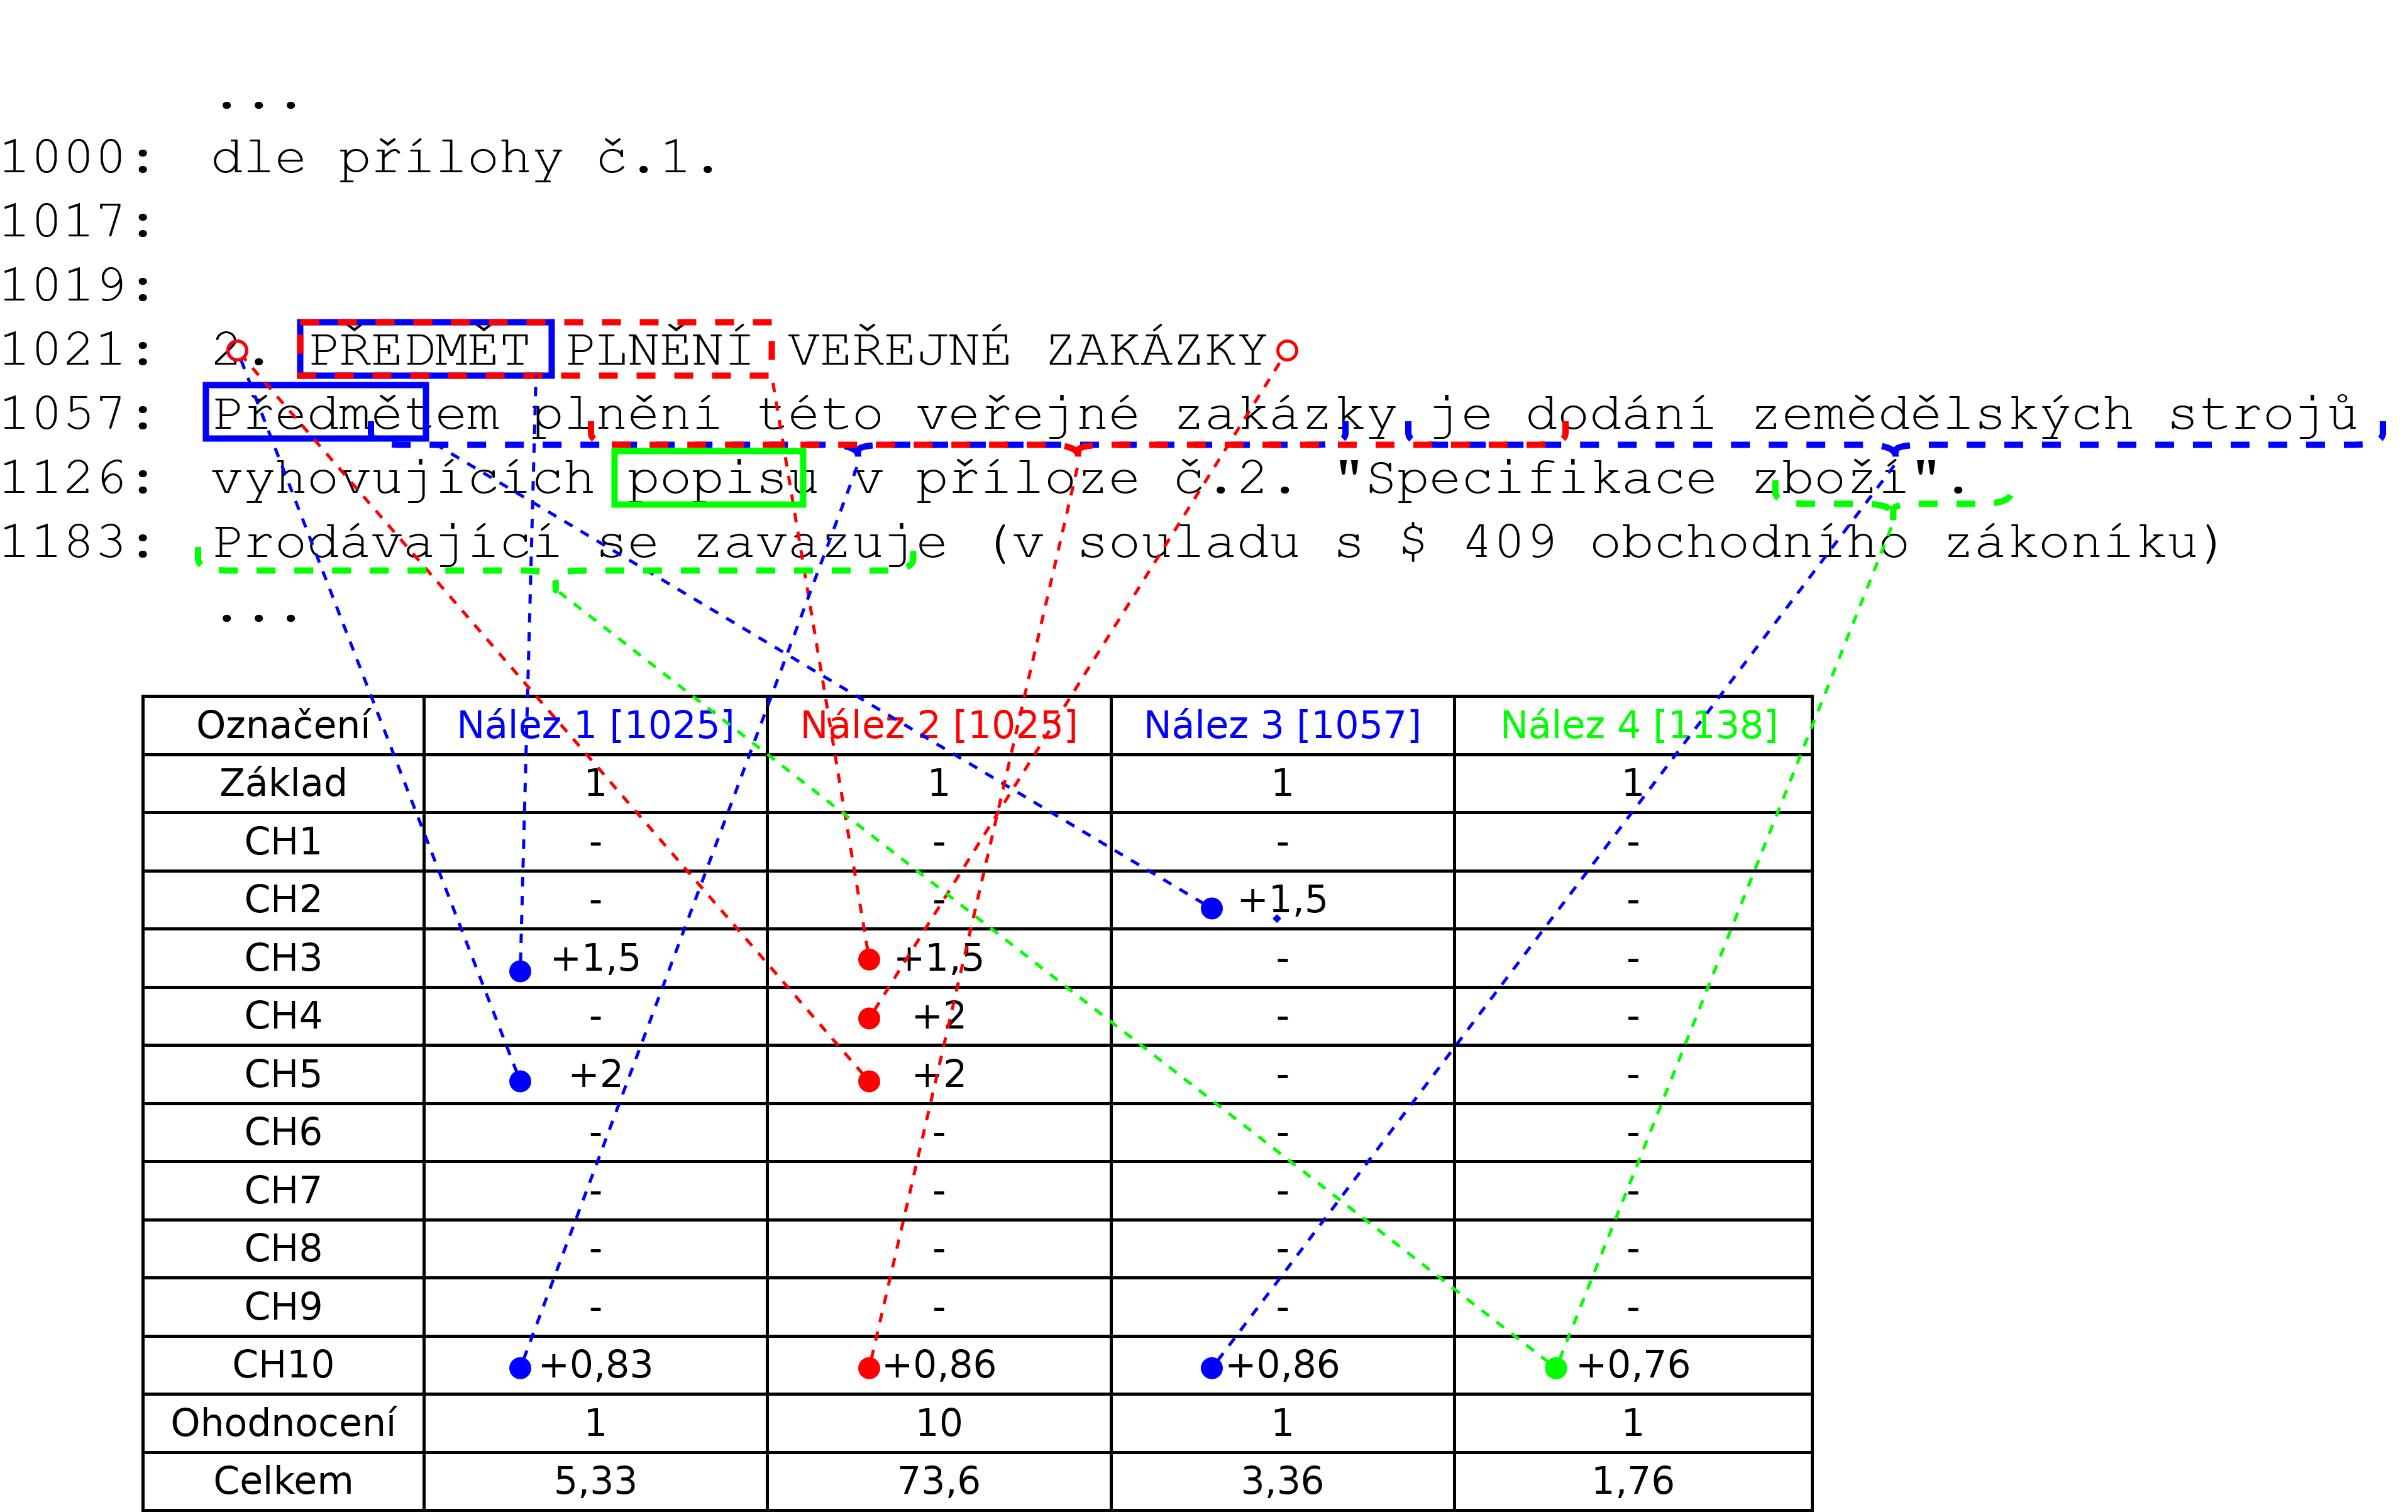
\includegraphics[width=1\textwidth]{images/subj_context_start.png}
    	\caption[Příklad výpočtu ohodnocení výskytů klíčových slov]{Příklad výpočtu ohodnocení výskytů klíčových slov\newline
    	Na příkladu jsou nalezeny dva nálezy klíčového slova \uv{Předmět} a jeden nález slova \uv{Předmět plnění}. Jsou detekovány charakteristiky přesného výskytu (CH2), verzálky (CH3), odřádkování (CH4) a číslování (CH5). V odstavci následuje běžná věta (CH10), což také v kladném smyslu ovlivňuje výsledné ohodnocení.}\label{fig:subjcontextstart}
    \end{figure}

    \item \textbf{Výběr nejlepších kandidátů}
    
    Pomocí samotného ohodnocení výskytů s ohledem na využití lokálních charakteristik je možné nalézt lokální maxima (např. nadpisy kapitol) avšak stále může docházet k falešným výskytům z textu odstavce (např. kumulací výskytů v odstavci). Ke zmírnění takového jevu implementuji algoritmus pro selekci nejlepšího možného výskytu na základě globálních statistik výskytů.
    
    Tento algoritmus spočívá v diskretizaci pomocí binningu a následné aplikace konvoluce s jádrem potlačujícím nežádoucí jevy.

    Diskretizaci provádím rozdělením celého textu na biny o stejné šířce, kterou odvozuji ze základní délky kontextu jako jeho třetinu (řádově tisíce znaků; defaultně 2040\footnote{Defaultní délku kontextu odvozuji expertním odhadem rozsahu kapitoly v počtu znaků (nízké tisíce) a zároveň s ohledem na dělitelnost velikostí konvolučního jádra (pro celočíselné rozdělování do binů)}: šíře binu je poté 680). Na tomto diskrétním prostoru počítám vážený histogram ohodnocení výskytů klíčových slov spadajících do jednotlivých binů.
    
    Následuje krok konvoluce, který z ohodnocení jednotlivých binů specifickým způsobem agreguje okolní biny jako skóre daného binu. Konvoluční jádro stanovuji na šestici (1, 1, 2, -2, -1, -1), která má za cíl určit samotný počátek kapitoly týkající se předmětu. Část (-2, -1, -1) penalizuje hodnoty tří předcházejících binů, zatímco část (1, 1, 2) agreguje tři následující s dvojnásobným umocněním prvního binu na pomyslném rozhraní kapitol.
    
    Některé VZ mají celý předmět rozdělen do několika podobně strukturovaných kapitol. Kvůli tomu nevybírám pouze bin s nejvyšším skóre, ale vybírám všechny biny, které dosahují alespoň dvou třetin maximálního dosaženého skóre.

% <příklad>
    % \begin{example}
        Navázáním na příklad z tabulky \ref{table:example_subj_keywords} a obrázku \ref{fig:subjcontextstart} dále znázorňuji na obrázku \ref{fig:subjcontextplot} výpočet histogramu. Výsledek aplikace konvoluce na histogram \ref{fig:subjcontextplot} je dále zobrazen na následujícím diagramu \ref{fig:subjcontextplot2}.
        
        \begin{figure}\centering
        	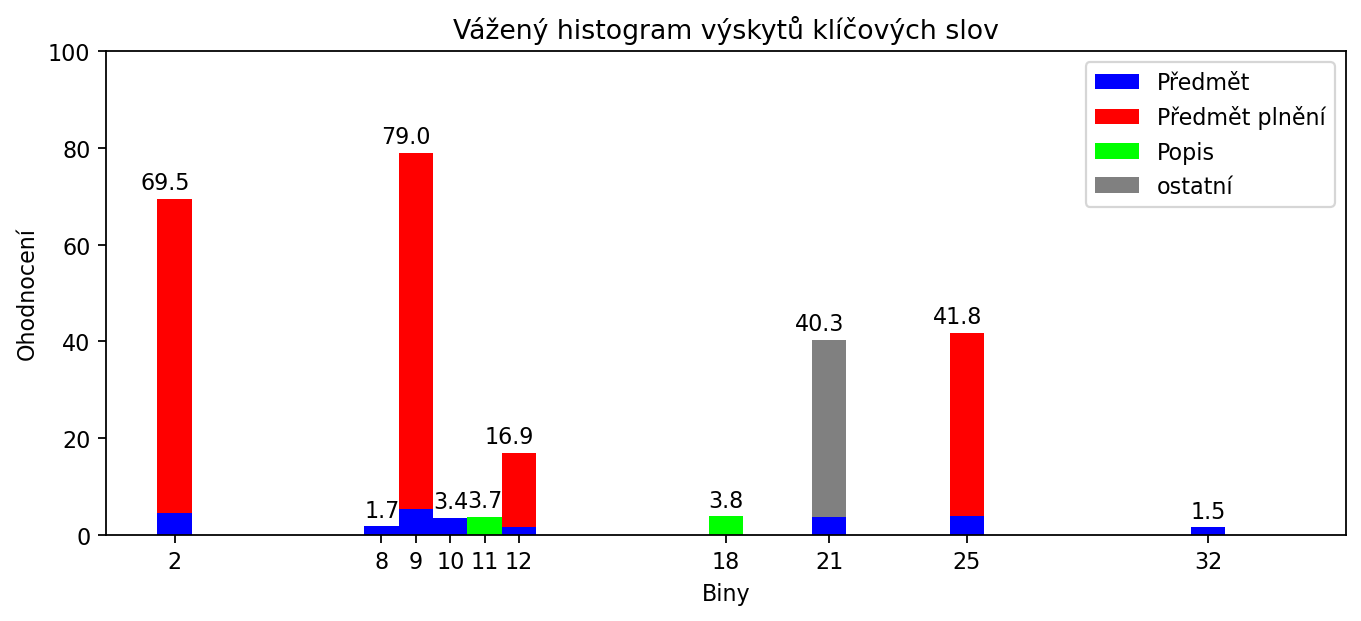
\includegraphics[width=1\textwidth]{images/subj_context_plot.png}
        	\caption[Histogram výskytů klíčových slov pro výběr kontextu]{Histogram výskytů klíčových slov pro výběr kontextu\newline
        	Biny jsou pro ilustraci o šíři 100 znaků (rozsah kontextu -- 300 znaků).  Úryvek z příkladu \ref{fig:subjcontextstart} je zde zastoupen biny 9 a 10, přičemž bin 9 nabývá nejvyššího ohodnocení.}\label{fig:subjcontextplot}
        \end{figure}
        
        \begin{figure}\centering
        	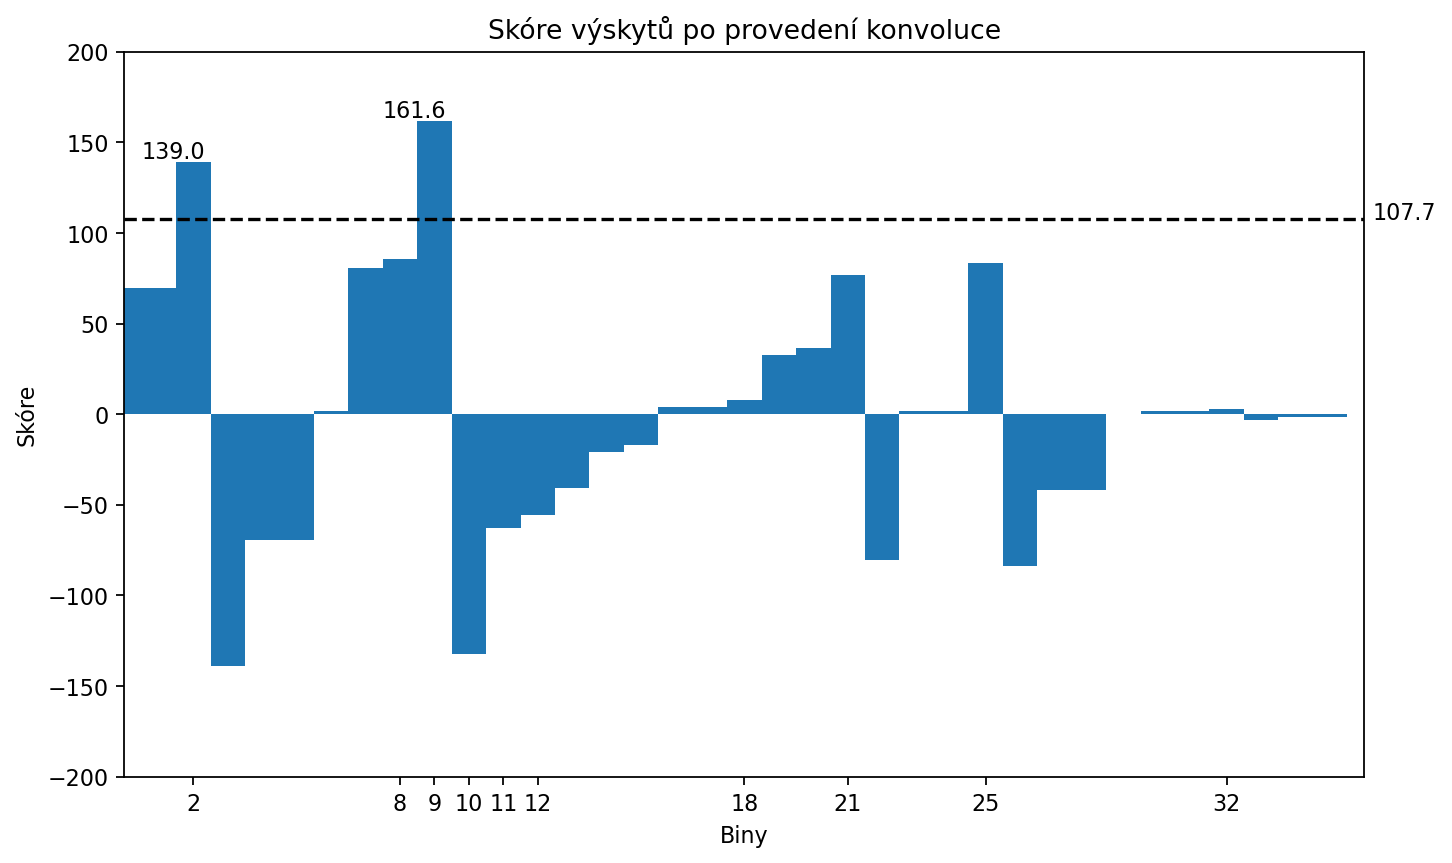
\includegraphics[width=1\textwidth]{images/subj_context_plot2.png}
        	\caption[Znázornění výběru nejlepších kandidátů na kontext podle skóre]{Znázornění výběru nejlepších kandidátů na kontext podle skóre\newline
        	Ohodnocení vnitřních binů kapitoly jsou potlačené (biny 10, 11, 12), zatímco v binu 9 jsou jejich výskyty agregovány a je zvýrazněna jeho důležitost pro výběr počátku kontextu. Horizontální čára znázorňuje rozhraní pro výsledný výběr binů 2 a 9.}\label{fig:subjcontextplot2}
        \end{figure}
    % \end{example}
    
    \item \textbf{Korekce samotného počátku kontextu}
    
    Po vzoru kroku 1. opakuji hledání výskytů těch samých klíčových slov v hrubě určených kontextech z předešlých kroků. Z těchto výskytů vybírám jeden nejvýznamnější, který se stává výsledným počátkem daného kontextu.
    
\end{enumerate}

\subsubsection{Určení konce kontextu}

Pouhý odhad ukončení kontextu na základě nastavené délky rozsahu je velice hrubá metoda, která v kontextu může zanechávat nežádoucí informace. Pokud však víme přesný počátek, můžeme na základě lokálního formátování takového počátku usuzovat, kde začíná další kapitola a stejně tak i určit, kde končí kontext předmětu.
\newpage

Následující detektory implementuji pro podchycení lokálního formátování počátků kapitol:
\begin{enumerate}
    \item Číslování kapitol
    
    Detektor detekuje hierarchické číslování kapitol na základě regulárního výrazu. Pokud je číslování detekováno, vypočítám číslo následující kapitoly, které dále detekuji v kontextu. Pokud dojde k pozitivnímu nálezu, určím jeho pozicí ukončení kontextu.
    
    \item Římské číslování kapitol

    Obdobný detektor, který místo klasických čísel pracuje s římskými čísly.

    \item Kapitoly uvedené klíčovým slovem
    
    Jednoduchý detektor, který hledá klíčové slovo \uv{článek} před počátkem kontextu. Pokud je slovo detekováno, je opět hledáno v kontextu a v případě nálezu určuje jeho ukončení.
    
    \item Název kapitoly psaný verzálkami
    
    Detektor detekuje, zdali je první řádek kontextu psaný velkými písmeny. Pokud ano, hledá další takový řádek a určí ho koncem kontextu.
    
    \item Pasáž uvedená klíčovým slovem
    
    V tomto případě nejde o určování konce kapitoly, nýbrž o ukončení předmětné fráze. Detektor hledá klíčové slovo \uv{název} kolem počáteční pozice, které předznamenává, že nejde o samostatnou kapitolu, ale jen o frázi s názvem předmětu. V takovém případě  ukončuji kontext s prvním odřádkováním za počátkem.
    
    \item Fráze v uvozovkách
    
    Pokud jsou detekovány za počátkem kontextu otevírací uvozovky, hledá detektor k nim do páru uzavírací symbol. Při nálezu je s ním kontext ukončen.
    
    \item Zakázaná klíčová slova
    
    Dokumentace VZ často kopírují podobnou strukturu. V mnoha případech se tak za kapitolou pojednávající předmět řeší cena, doba, či místo plnění. Na základě toho detektor detekuje klíčová slova: \uv{cena}, \uv{doba} a \uv{místo} a jejich případným nálezem ukončuje kontext.
    
    \item Defaultní odhad délky
    
    V případě selhání všech předešlých detektorů zůstává kontext ukončený nastavenou maximální délkou.
    
\end{enumerate}

% <příklad>
\begin{example}
    Pro příklad nálezu kontextu v úryvku \ref{fig:subjcontextstart} by se aplikovaly detektory 1 a případně 4.
\end{example}

\subsubsection{Měření dopadu jednotlivých algoritmů a jejich parametrů}

Měření provádím oproti množině 40 pseudo-náhodně vybraných veřejných zakázek, u kterých jsem manuálně validoval výstup extrakce. Jako metriku pro podobnost vyextrahovaného a referenčního textu používám Jaccard index (viz. kapitola \ref{sec:text_sim_metrics}).

Pro každou VZ aplikuji tuto metriku a nakonec počítám výsledné skóre jako jejich průměr.

V následujících tabulkách jsou zaznamenány výsledky měření pro jednotlivá klíčová slova, lokální charakteristiky a detektory. Uvedené doby běhu jednotlivých měření jsou pouze orientační. Vždy provádím měření pouze \uv{s} danou entitou a \uv{bez} ní (se všemi ostatními).

\begin{table}[h!]
\centering
\begin{tabular}{ |l|r|r|r|r| }
\hline
 & \multicolumn{2}{|c|}{Pouze jedno} & \multicolumn{2}{|c|}{Bez jednoho} \\\hline
Klíčové slovo (ohodnocení) & Skóre & Čas [s] & Skóre & Čas [s] \\\hline
\hline
Vše & 100.00 & 12.1 & - & - \\\hline
Předmět smlouvy (10) & 44.98 & 1.4 & 68.01 & 11.5 \\
Předmět díla (10) & 7.52 & 0.5 & 94.97 & 11.5\\
Předmět plnění (10) & 14.81 & 1.8 & 88.50 & 11.9\\
Předmět veřejné zakázky (10) & 20.32  & 0.7 & 89.02 & 13.1\\\hline
Vymezení předmětu (10) & 8.76 & 0.4 & 93.84 & 12.6\\
Vymezení plnění (10) & 2.61 & 0.5 & 97.57 & 12.5\\
Popis předmětu (10) & 12.52 & 0.7 & 97.05 & 12.5\\
Název veřejné zakázky (3) & 12.88 & 2.0 & 92.28 & 11.2\\\hline
Veřejná zakázka (1) & 8.79 & 3.2 & 98.46 & 11.2\\
Veřejné zakázce (1) & 13.22 & 1.6 & 96.02 & 11.0\\
Předmět (1) & 66.11 & 7.0 & 97.51 & 6.4\\
Popis (1) & 10.64 & 4.1 & 98.96 & 8.4\\\hline
\end{tabular}
\caption{Měření dopadu jednotlivých klíčových slov na extrakci}
\label{table:experiment_subj_keywords}
\end{table}

V tabulce \ref{table:experiment_subj_keywords} můžeme vidět, jaký dopad na přesnost extrakce předmětu mají jednotlivá klíčová slova. Je vidět, že slovo \uv{předmět} a \uv{popis} zatěžují extrakci nejvíce, což bude zřejmě přímo implikováno počtem jejich výskytů. Z měření je dále zřejmé očekávané chování slova \uv{předmět}, které samo o sobě dokáže do jisté míry podchytit kontext, zatímco na jeho přesné určení má malý vliv. Oproti tomu, sousloví \uv{předmět smlouvy} má nejznatelnější dopad na upřesnění kontextu.

\begin{table}[h!]
\centering
\begin{tabular}{ |l|r|r|r|r| }
\hline
 & \multicolumn{2}{|c|}{Pouze jedna} & \multicolumn{2}{|c|}{Bez jedné} \\\hline
Charakteristika & Skóre & Čas [s] & Skóre & Čas [s] \\\hline
\hline
Základ/Vše & 64.48 & 12.9 & 100.00 & 10.6\\\hline
CH1 & 78.95 & 12.0 & 96.53 & 11.6\\
CH2 & 77.30 & 12.2 & 97.13 & 11.9\\
CH3 & 64.82 & 12.2 & 98.73 & 11.4\\
CH4 & 77.72 & 11.9 & 98.73 & 11.4\\
CH5 & 65.21 & 11.3 & 89.89 & 12.1\\\hline
CH6 & 72.12 & 11.6 & 94.79& 11.4\\
CH7 & 64.25 & 11.9 & 98.60 & 11.8\\
CH8 & 72.13 & 11.9 & 97.76 & 11.5\\
CH9 & 64.75 & 11.2 & 99.08 & 12.2\\
CH10 & 62.71 & 12.1 & 97.70 & 11.1\\\hline
\end{tabular}
\caption{Měření dopadu jednotlivých lokálních charakteristik na extrakci}
\label{table:experiment_characteristics}
\end{table}

V tabulce \ref{table:experiment_characteristics} je vidět dopad jednotlivých lokálních charakteristik pro úpravu koeficientu ohodnocení výskytů klíčových slov. Ani jedna charakteristika nemá obzvlášť citelný dopad na výpočetní náročnost. Sama o sobě má největší vliv CH1 -- nález obsahuje samostatnou řádku, zatímco největší dopad na upřesnění kontextu má potom CH5 -- číslování kapitol (zároveň i CH6 -- římské číslování má druhý největší dopad).

\begin{table}[h!]
\centering
\begin{tabular}{ |l|r|r|r|r| }
\hline
 & \multicolumn{2}{|c|}{Pouze jeden} & \multicolumn{2}{|c|}{Bez jednoho} \\\hline
Detektor & Skóre & Čas [s] & Skóre & Čas [s] \\\hline
\hline
Základ/Vše & 34.14 & 11.0 & 100.00 & 12.1\\\hline
1 & 58.40 & 11.6 & 83.73 & 12.5\\
2 & 58.40 & 11.6 & 90.96 & 12.3\\
3 & 39.30 & 11.6 & 97.83 & 12.4\\
4 & 40.88 & 12.6 & 98.71 & 12.2\\\hline
5 & 40.81 & 12.0 & 93.83 & 12.2\\
6 & 36.47 & 11.9 & 97.67 & 12.4\\
7 & 61.64 & 12.2 & 91.69 & 12.2\\\hline
\end{tabular}
\caption{Měření dopadu jednotlivých detektorů na extrakci}
\label{table:experiment_detectors}
\end{table}

Nakonec v tabulce \ref{table:experiment_detectors} můžeme pozorovat dopad detektorů ukončení kontextu. Nejvýznamnější dopad mají detektory 1 a 2 (detektory klasického respektive římského číslování kapitol. Dobře také funguje detektor 7 -- ukončovací klíčová slova. V tabulce lze pozorovat zvláštní jev u prvních dvou detektorů, které mají stejné skóre i čas. Podle mého úsudku je to způsobené chybou v měření.


\subsection{Filtrování a transformace kontextu předmětu}
\label{sec:subj_filtering}

Veliké množství dokumentace veřejných zakázek je uveřejněno ve formátu oskenovaných papírových dokumentů. Z takových dokumentů extrahuji text pomocí OCR technologie, což do prostého textu zanáší různý šum, jako například záhlaví/zápatí stran, špatné odřádkování a členění textu, či chybně rozpoznané znaky.

Kvůli tomu je potřeba před samotnou extrakcí předmětných částí provést různá filtrování, transformace či případné korekce daného kontextu předmětu. Tento proces tak vstupní kontext v původní podobě zpracovává do čisté podoby.

Jak je vidět na schéma \ref{fig:subjextraction}, proces sériově aplikuje jednotlivé procesory (filtery/transformery), kde výstup jednoho přichází jako vstup do následujícího. Jelikož jsou některé procesory závislé na předchozích, záleží na pořadí jejich aplikace.

Účel mnoha procesorů je intuitivní, zatímco některých tolik ne. To může být způsobeno tím, že některé procesory implementuji za účelem přípravy vstupu pro algoritmy extrakce a tagovací model, který je citlivý na čistotu textu. Tento model používám dále při extrakci podle větného rozboru vět (více viz. kapitola \ref{sec:sentence_dependency_extraction}).

Dále popisuji jednotlivé procesory v pořadí, v jakém je aplikuji.
\begin{enumerate}
    \item Odstranění číselných řádků
    
    Řádky s nadpolovičním poměrem číselných znaků jsou pravděpodobně řádky obsahující nerelevantní text (např. identifikátory, ceny).
    
    \item Odstranění příliš krátkých řádků
    
    Neprázdné řádky kratší šesti znaků jsou pravděpodobně jen pozůstatky formátovaného textu a nenesou žádnou hodnotnou informaci.
    
    \item Odstranění nerelevantních řádků
    
    Za použití klíčových slov a regulárních výrazů definuji několik podmínek charakterizující nerelevantní řádky, jako jsou:
    \begin{itemize}
        \item stránkování,
        \item telefonní čísla a fax,
        \item obchodní identifikátory,
        \item webové a emailové adresy.
    \end{itemize}
    
    \item Korekce interpunkce na konci vět
    
    Pomocí regulárního výrazu detekuji chybné čárky na místech, kde je očekávaná tečka.
    
    \item Odstranění číslování odstavců
    
    Opět za použití regulárního výrazu odmazávám z počátků řádů číslování.
    
    \item Filter prázdných řádků
    
    Na základě délky řádků implementuji algoritmus odstranění zavádějícího odřádkování způsobeného chybnou extrakcí textu. Více v kapitole \ref{sec:blank_lines_filter}.
    
    \item Sjednocení symbolů pro uvozovky
    
    Nahrazení českých znaků pro uvozovky univerzálním znakem ".
    
    \item Transformace příliš dlouhých řádků
    
    Na základě výskytu specifických znaků a délky řádků transformuji vybrané řádky do několika kratších. Více v kapitole \ref{sec:too_long_lines_transformer}
    
    \item Doplnění teček na konce řádků
    
    Jeden z transformerů implementovaných z důvodů přípravy textu pro tagovací model.
    
    \item Doplnění dvojteček
    
    Transformer připravující text pro extrakci podle lokálních statistik. Detekuje situaci, kde se vyskytuje klíčové slovo \uv{název} či \uv{popis} před názvem entity s počátečním velkým písmenem. V takové situaci doplňuje před název dvojtečku.
    
    \item Nahrazení dvojtečky za dvojici \uv{:.}
    
    Další transformer připravující text pro tagovací model.
    
    \item Nahrazení vícenásobných teček za jednu.
    
    Obdobně jako předchozí transformer.
    
    \item Odstranění textu v závorkách
    
    V závorkách je obvykle uvedena pouze dodatečná informace, která zpravidla není předmětná. Pomocí regulárního výrazu tak závorky odstraňuji i s textem, který obsahují.
    
\end{enumerate}

\subsubsection{Filter prázdných řádků}
\label{sec:blank_lines_filter}

U některých dokumentů dochází při extrakci textu ke špatně rozpoznanému odřádkování. V extrémních případech až do té míry, že jednotlivé řádky jsou oddělené několika odřádkováními, přestože text souvisle navazuje ve větách. Na druhou stranu, odřádkování obecně mají v textu svůj význam a i v případě extrakce textu mohou přinášet užitečnou informaci (více v kapitole \ref{sec:local_stats_extraction}).

Pro zaručení správného fungování extraktorů je nutné potlačit jev falešných odřádkování. To zajišťuje tento filter, kterým se v ideálním případě snažím dosáhnout toho, aby souvislá věta nebyla vůbec rozdělena odřádkováním.

Nejdříve je potřeba detekovat, zdali se v textu vyskytují nějaká falešná odřádkování a následně tato odřádkování potlačit.

Pro detekci výskytu falešných odřádkování v textu implementuji algoritmus založený na globální statistice délek řádků. Myšlenka algoritmu spočívá v tom, že dokument bez falešných odřádkování má veliký rozptyl délek řádků, zatímco dokument, který má falešná odřádkování (např. odřádkování podle šíře listu papíru) má tento rozptyl malý. Algoritmus se skládá z následujících čtyř kroků:

\begin{enumerate}
    \item Určím délku plného řádku v počtu znaků. Kvůli potlačení extrémů nevybírám maximální délku, ale délku řádku odpovídající kvantilu = 0,95 (do množiny nezapočítávám prázdné řádky).
    \item Vzhledem k tomu, že v dokumentaci se běžně používá proporcionálního písma, plné řádky mohou dosahovat znatelně odlišných délek. Takovou odchylku definuji expertním odhadem na 15 \%, podle čeho určuji rozhraní pro výběr všech \uv{plných} řádků jako alespoň 85 \% délky určené v předchozím kroku.
    \item Pokud je množina \uv{plných} řádků dostatečně veliká, odebírám maximální a minimální prvek pro stabilnější statistiku. U výsledné množiny počítám standardní odchylku jejich délek.
    \item Pokud je tato odchylka menší než nastavená hranice (defaultně 5), detekuji text jako \uv{obsahující falešné řádky} a je dále zpracován pro jejich potlačení.
\end{enumerate}

Oproti algoritmu detekce výskytu falešných odřádkování, algoritmus na jejich samotné potlačení je založený na lokální statistice délek řádků se základní myšlenkou takovou, že pokud se za sebou vyskytuje několik \uv{plných} řádků, odřádkování mezi nimi jsou falešná a je žádoucí je odstranit.

Výčet podmínek pro zrušení (falešných) odřádkování je následující:
\begin{enumerate}
    \item pokud poslední řádka\footnote{Poslední řádkou je myšlena poslední neprázdná řádka včetně řádky aktuálně řešené, nebo řádka prázdná, ovšem rozpoznaná jako nefalešná.} je zároveň \uv{plná} a tvoří běžnou větu (má poměr malých písmen větší něž určená hranice - defaultně 0,6), nebo
    \item pokud poslední řádka nekončí ukončením věty (tečka na jejím konci) a~zároveň jí předcházející řádka je \uv{plná}, nebo
    \item pokud následující řádka je \uv{plná} a nezačíná novou větou (velké písmeno na začátku),
    \item nakonec nahrazuji všechna vícenásobná odřádkování právě dvěma.
\end{enumerate}

Těmito podmínkami jsem schopen podchytit většinovou část falešných odřádkování, a to i u takových řádek, které ruší souvislý blok \uv{plných} řádek tím, že sama není \uv{plná}.

% <příklad>
% \begin{example}
    Pro příklad uvádím na obrázku \ref{fig:blanklinesfilter} ilustraci algoritmu na úryvku textu. Na obrázku \ref{fig:blanklinesfilteoutr} je poté znázorněn výsledný text po aplikaci filteru, kde je vidět, že zbyly pouze nefalešné odřádkování.
    
    \begin{figure}\centering
    	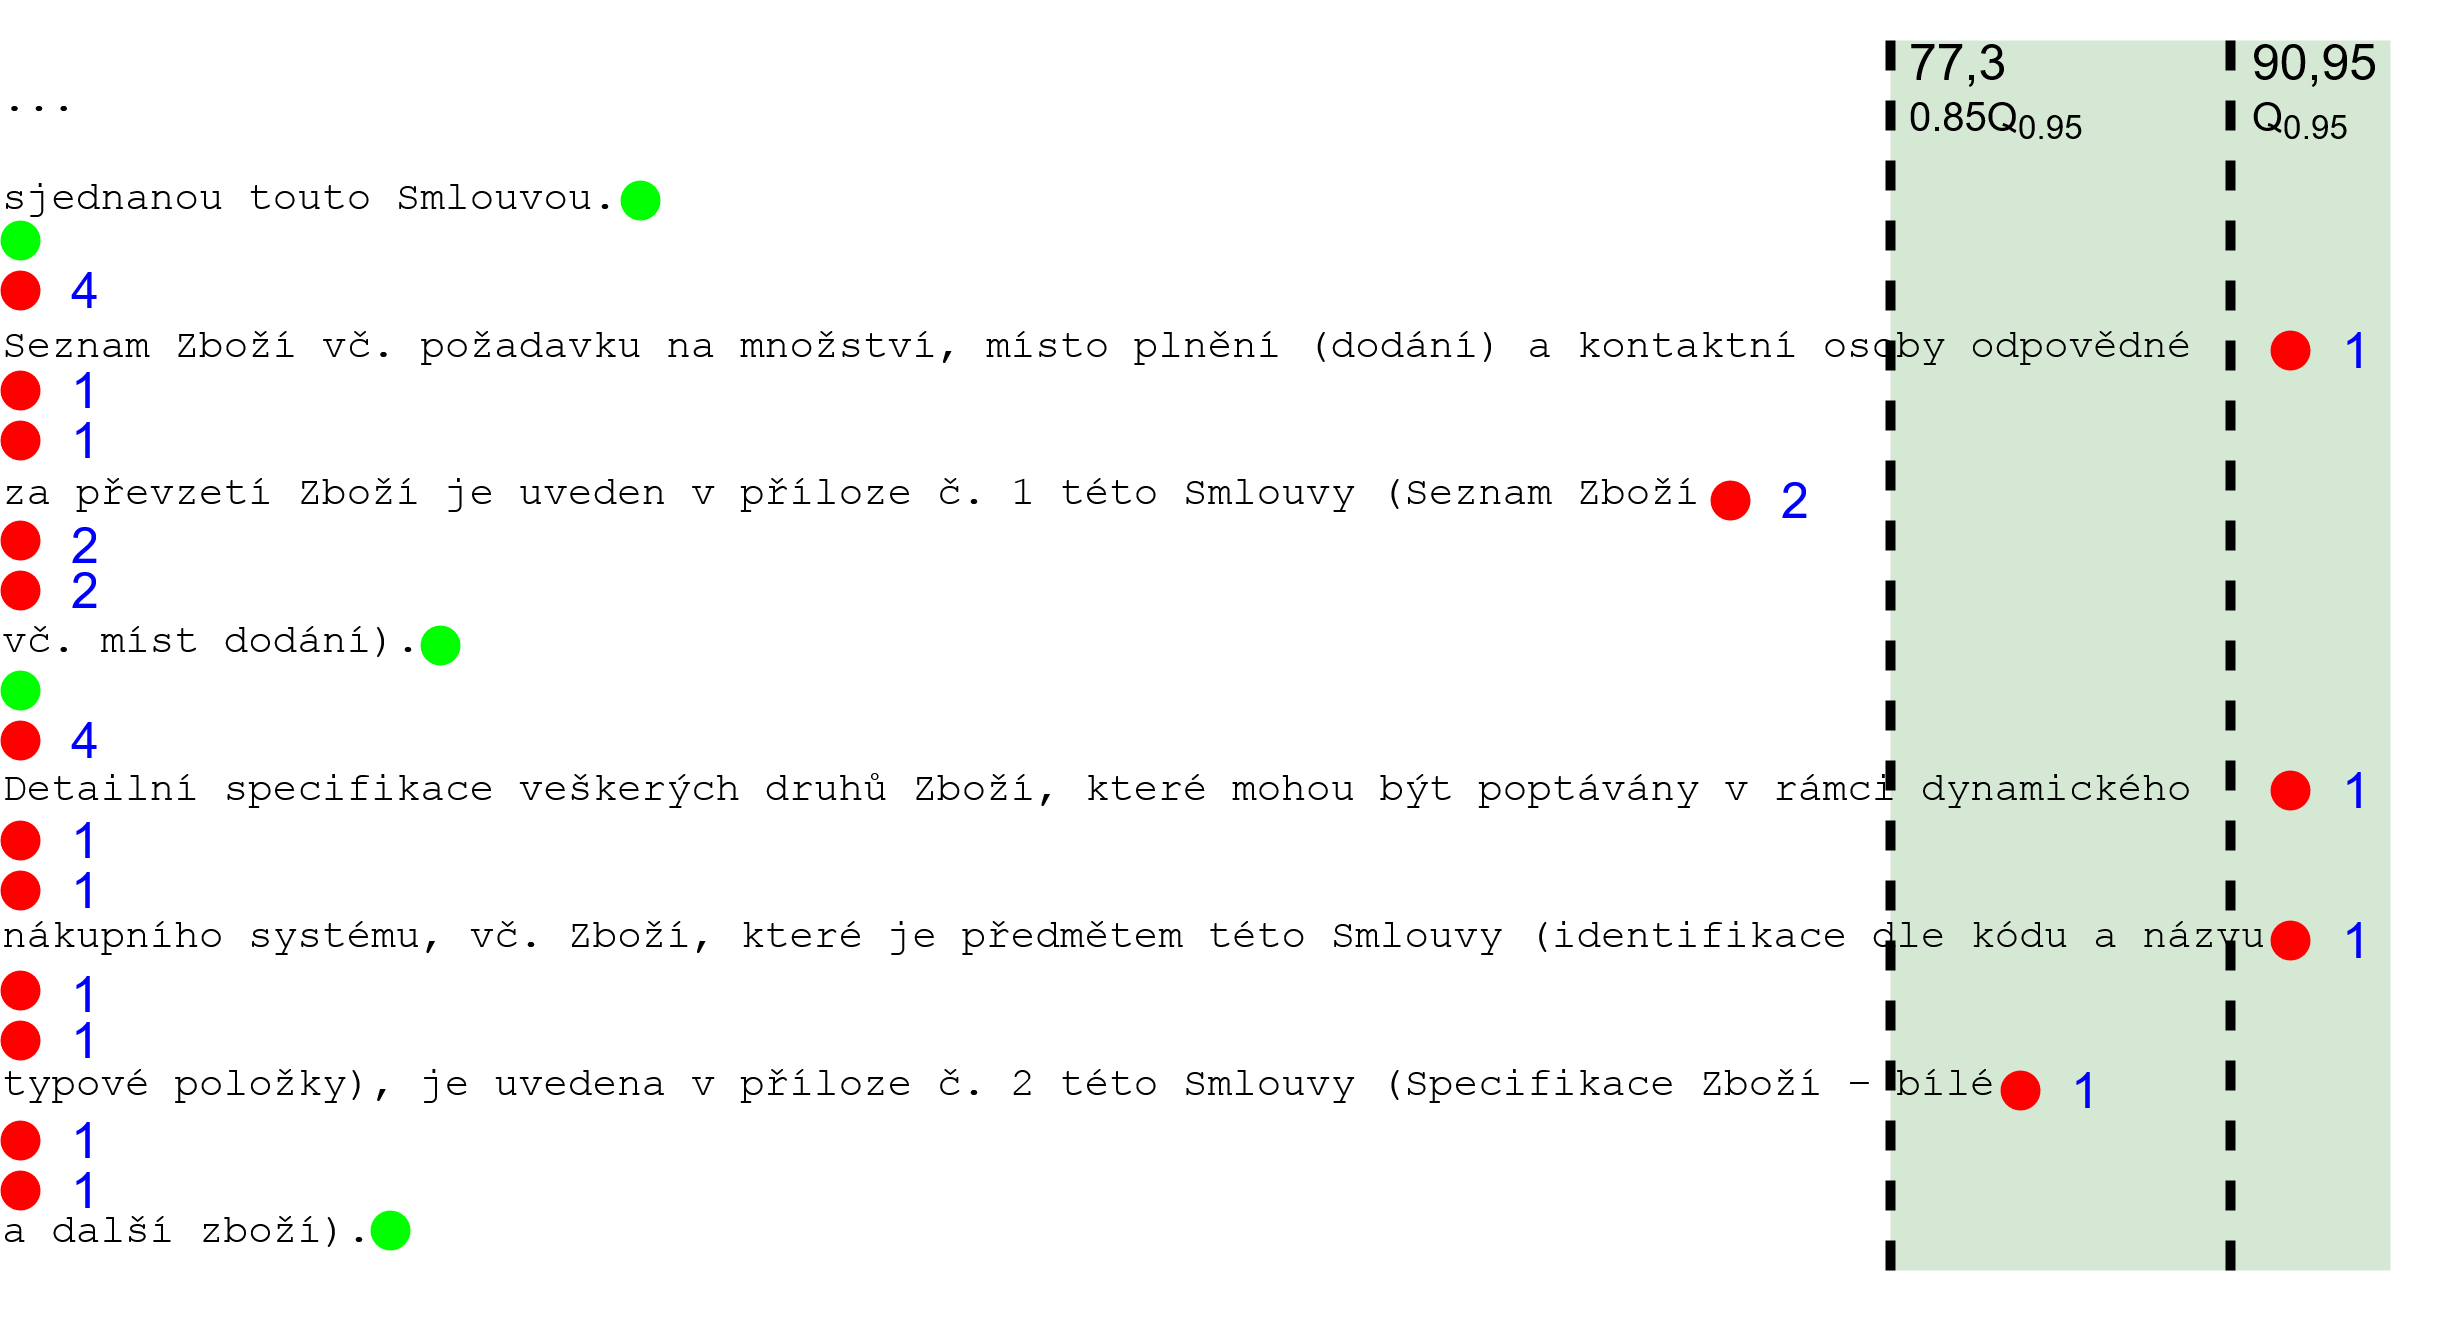
\includegraphics[width=1\textwidth]{images/blank_lines_filter.png}
    	\caption[Ilustrace algoritmu filtru prázdných řádek]{Ilustrace algoritmu filtru prázdných řádek\newline
    	Falešná a nefalešná odřádkování jsou označena červenými, respektive zelenými body. Je vidět detekce \uv{plných} řádek jako řádek delších 77 znaků. Modrými čísly je nakonec naznačeno, která podmínka se uplatňuje pro zrušení odřádkování.}\label{fig:blanklinesfilter}
    \end{figure}
    
    \begin{figure}\centering
    	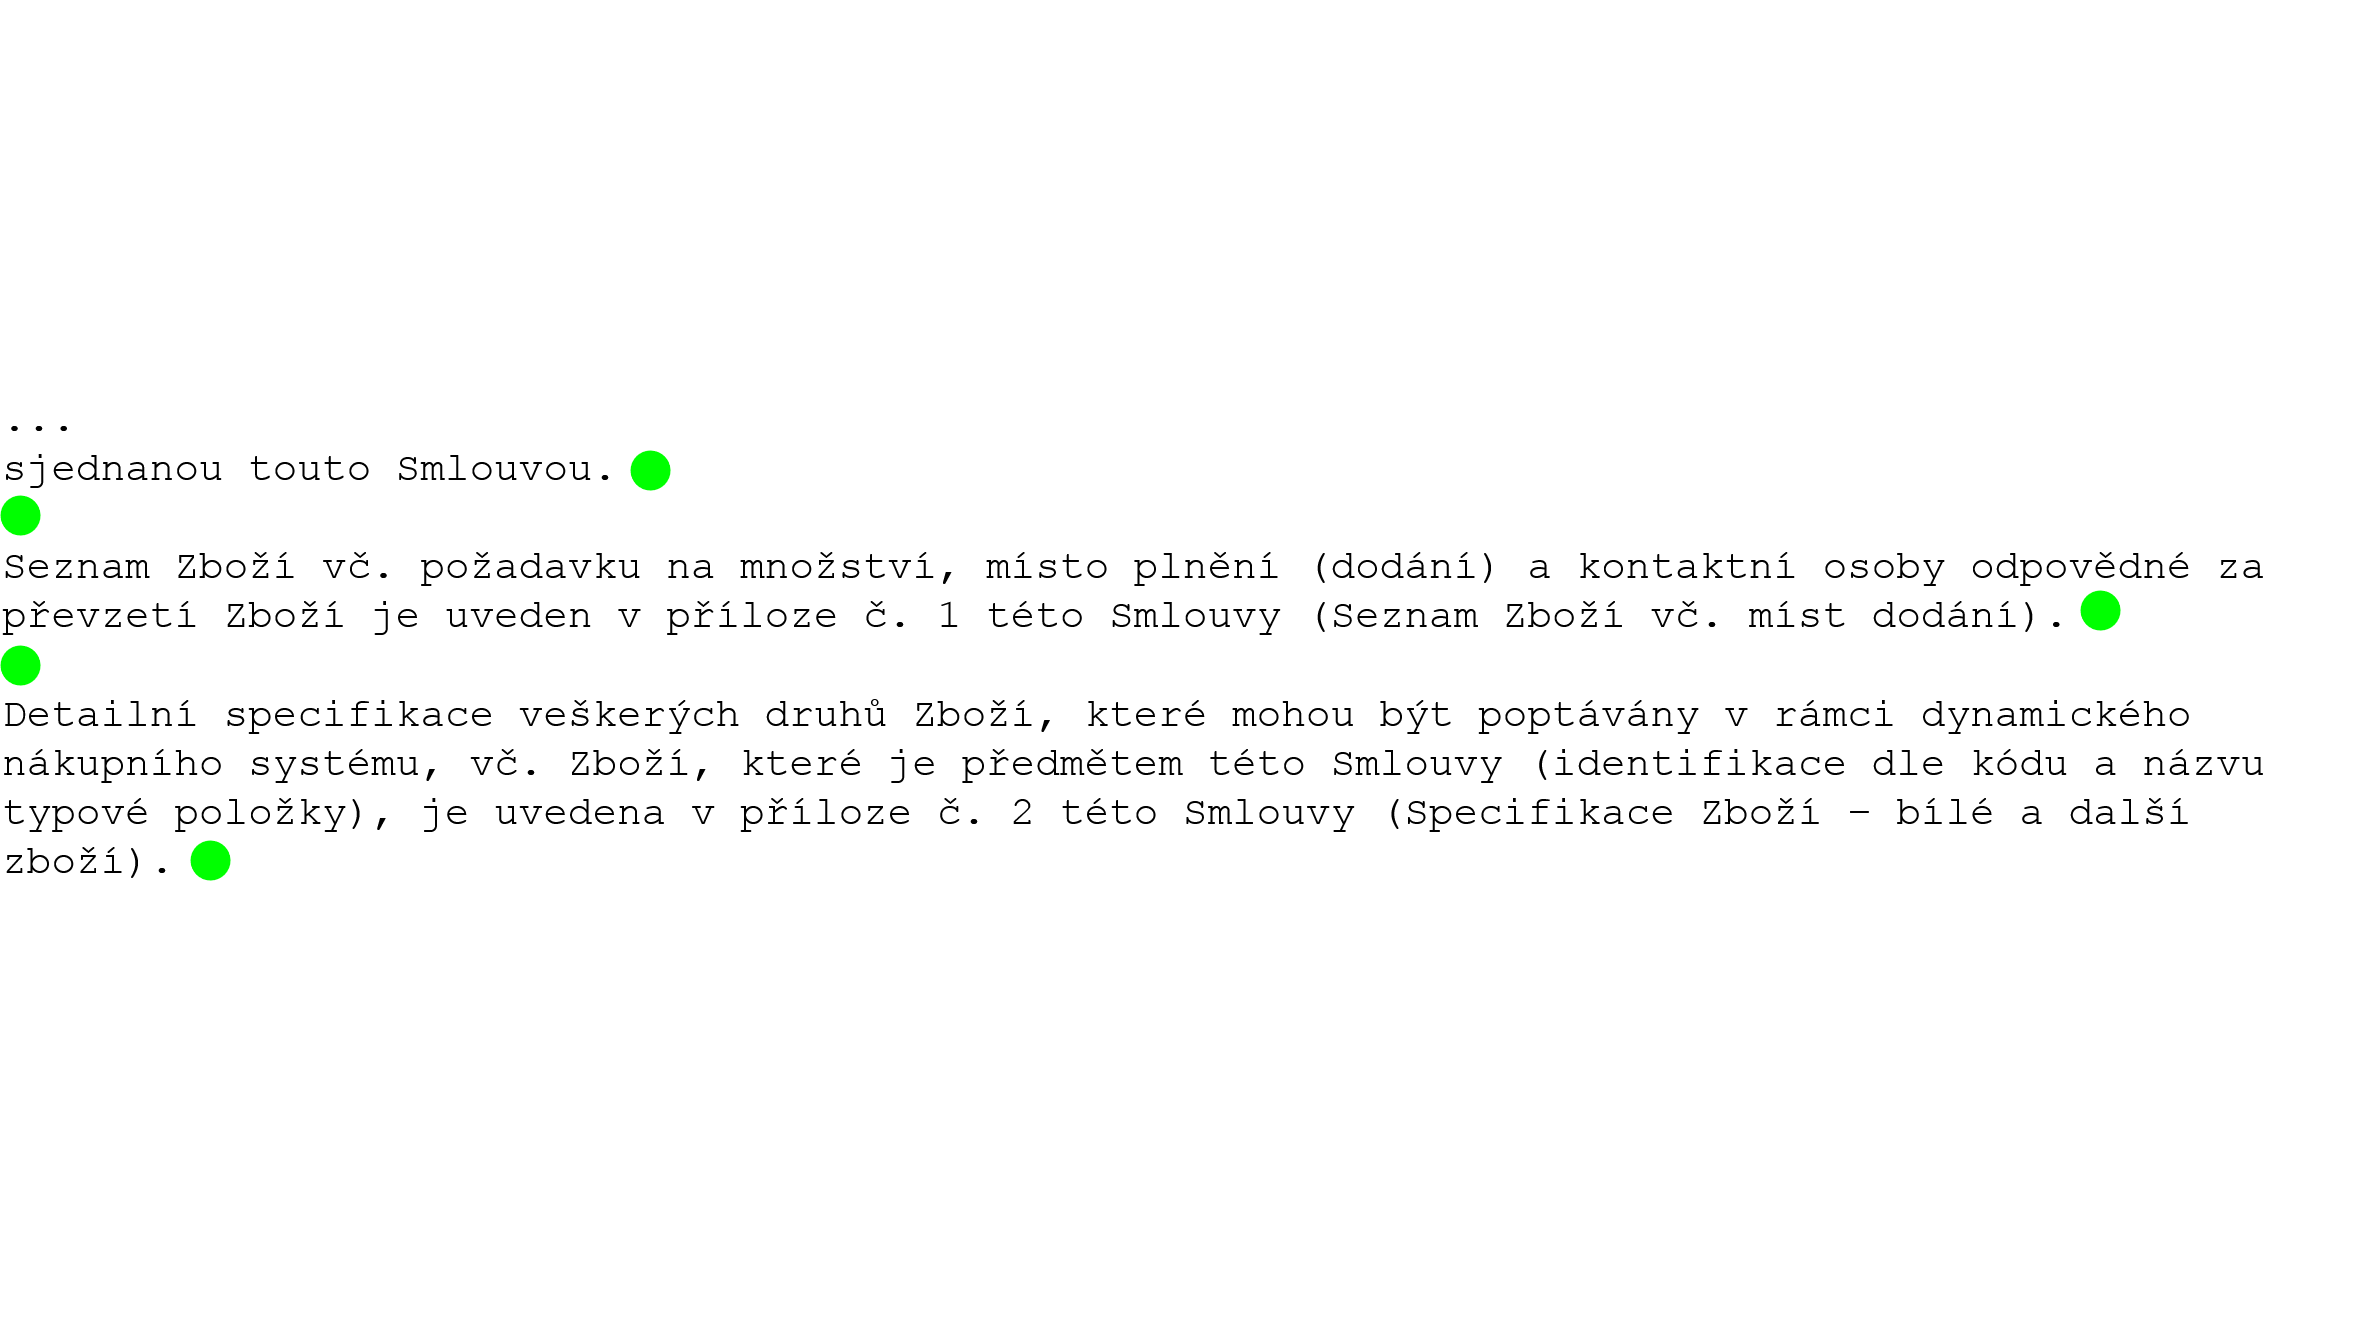
\includegraphics[width=1\textwidth]{images/blank_lines_filter_out.png}
    	\caption{Ilustrace výsledku algoritmu filtru prázdných řádek}\label{fig:blanklinesfilteoutr}
    \end{figure}
% \end{example}




\subsubsection{Transformer příliš dlouhých řádků}
\label{sec:too_long_lines_transformer}

U některých řádků dochází k jevu, že tvoří dlouhý souvislý řetězec, ačkoli by mohly být rozděleny do více kratších řádků. Například řádek obsahující více pomlček je vhodné rozdělit do několika bodově strukturovaných řádků.
% K tomu navíc může docházet častěji po aplikaci filtru prázdných řádků z předchozí kapitoly. 

Takové rozdělování řeší tento transformer, který detekuje znaky tvořící odrážkovou/výčtovou strukturu a následně do takové struktury člení řádky, ve kterých se detekované znaky vyskytují.

Implementuji algoritmus, který nejprve detekuje znaky tvořící výčtovou strukturu a poté rozděluje řádky je obsahující. Kromě tzv. \uv{bílých znaků} počítám výskyty prvních znaků všech řádek. Z napočítané množiny vybírám nejpočetnější nealfanumerický znak a podle něj rozděluji řádky, ve kterých se vyskytuje (kromě výskytů v uvozovkách).

\subsubsection{Měření dopadu jednotlivých filterů a transformerů}
\label{sec:filter_transformer_measurements}

Podobně jako u procesu extrakce kontextu provádím měření dopadu jednotlivých filterů a transformerů na extrakci předmětu. Používám stejnou množinu dokumentů i metriku. Jako referenční data používám manuálně ověřenou a opravenou množinu výstupu celého procesu extrakce předmětu.

\begin{table}[h!]
\centering
\begin{tabular}{ |l|r|r|r|r| }
\hline
 & \multicolumn{2}{|c|}{Pouze jeden} & \multicolumn{2}{|c|}{Bez jednoho} \\\hline
Procesor & Skóre & Čas [s] & Skóre & Čas [s] \\\hline
\hline
Základ/Vše & 35.57 & 38.1 & 78.53 & 35.2\\\hline
1 Odstranění číselných řádků & 35.32 & 36.5 & 75.73 & 36.9\\
2 Odstranění příliš krátkých řádků & 39.20 & 36.6 & 72.92 & 35.7\\
3a Odstranění stránkování & 36.08 & 40.3 & 76.52 & 35.0\\
3b Odstranění telefonních čísel & 35.40 & 38.3 & 77.71 & 34.4\\
3c Odstranění obchodních identifikátorů & 35.66 & 38.4 & 78.53 & 34.5\\\hline
3d Odstranění webových adres & 35.58 & 37.0 & 78.02 & 34.3\\
4 Korekce interpunkce & 35.65 & 39.4 & 77.59 & 34.3\\
5 Odstranění číslování odstavců & 36.93 & 40.1 & 78.09 & 34.7\\
6 Filter prázdných řádků & 37.52 & 42.5 & 55.51 & 34.1\\
7 Sjednocení uvozovek & 45.53 & 41.6 & 63.79 & 34.4\\\hline
8 Transformace příliš dlouhých řádků & 35.50 & 39.5 & 75.07 & 35.4\\
9 Doplnění teček & 33.30 & 41.5 & 75.87 & 34.7\\
10 Doplnění dvojteček & 35.72 & 41.7 & 78.36 & 34.7\\
11 Nahrazení dvojteček & 43.56 & 40.7 & 75.36 & 34.7\\
12 Nahrazení teček & 43.56 & 37.2 & 77.71 & 35.0\\
13 Odstranění závorek & 37.64 & 37.2 & 74.11 & 35.6\\\hline
\end{tabular}
\caption{Měření dopadu jednotlivých filterů a transformerů na extrakci předmětných položek}
\label{table:experiment_transformers}
\end{table}

V tabulce \ref{table:experiment_transformers} je vidět výsledky měření. Změny časů napovídají, že některé procesory urychlují výslednou dobu běhu procesu extrakce. Zároveň je také vidět, že téměř všechny procesory mají vliv na přesnost extrakce. Jediný procesor, který nezlepšuje skóre je procesor 3c, který ve validační množině dokumentů zřejmě nenašel uplatnění.


\subsection{Extrakce podle lokálních charakteristik}
\label{sec:local_stats_extraction}

V předešlých kapitolách jsem narážel na fakt, že přestože je většina formátování zdrojového textu extrahováním ztracena, některé charakteristiky zůstávají a lze je využít. Přesně o to se snažím tímto procesem, jak dále popisuji v této kapitole.

Položky předmětu bývají často v dokumentaci vyjmenované v seznamech strukturovaných odrážkami či odřádkováními. Takové seznamy se snažím pomocí následujících extraktorů detekovat a extrahovat. Kromě seznamů se dále zaměřuji na název zakázky, který často sám o sobě nese předmětnou informaci. Výstupem tohoto procesu tak je výčet konkrétních předmětných položek a názvů.

\newpage
Extraktory sloužících k účelům tohoto procesu jsou následující:
\begin{enumerate}
    \item Výčet položek podle struktury odřádkování
    
    Extraktor detekuje vzor v odřádkování a podle takového vzoru vrací výčet položek (více viz. kapitolu \ref{sec:structure_item_enumeration_extractor}).
    
    \item Výčet položek podle odrážek
    
    Extraktor využívá podobný algoritmus detekce znaků tvořících odrážky jako transformer příliš dlouhých řádků (viz. kapitola \ref{sec:too_long_lines_transformer}) a podle těchto odrážek extrahuje položky. Více do detailu popisuji v samostatné kapitole \ref{sec:char_item_enumeration_extractor}.
    
    \item Rozšíření výčtu položek
    
    Zde nejde o extraktor samotný, ale o rozšíření dvou předešlých. Nalezené výčty jsou obvykle uvozené nadpisem, nebo větou, čeho se týkají. Takové uvození detekuje toto rozšíření, které v několika řádcích před nalezeným výčtem hledá specifické znaky (například dvojtečku) a výčet tak rozšiřuje o položky, které se vyskytují mezi nalezenou dvojtečkou a počátkem detekovaného výčtu.
    
    \item Položka za speciálním znakem
    
    Předmět zakázky se může skládat pouze z jedné položky. V takových případech bývá položka vyjmenovaná v řádku za nějakým specifickým znakem (například dvojtečkou). Takovou situaci detekuji a v případě nálezu obsah za znakem vracím jako samostatnou položku předmětu.
    
    \item Položka za klíčovým slovem
    
    Obdobně jako předešlý extraktor funguje i tento s tím rozdílem, že místo specifického znaku detekuje specifické klíčové slovo (vzor regulárního výrazu).
    
    \item Název zakázky v uvozovkách
    
    Extraktor extrahuje obsah závorek jako název zakázky, pokud se před závorkou vyskytuje jedno z nastavených klíčových slov (např. \uv{název}) a zároveň se nevyskytuje žádné ze zakázaných.
    
    \item Strukturovaný název zakázky
    
    Obdobně jako u extraktoru položky za speciálním znakem extrahuji i~název zakázky. Navíc zde opět kontroluji pozitivní a negativní klíčová slova.
\end{enumerate}




\subsubsection{Výčet položek podle struktury odřádkování}
\label{sec:structure_item_enumeration_extractor}

Při extrakci textu se výčty položek obvykle převedou na jednotlivé položky pravidelně prokládané odřádkováními. Navíc, díky filtrování a transformaci kontextu, je taková pravidelnost až na výjimky zaručená. Na základě toho implementuji následující algoritmus, který detekuje delší úseky pravidelného vzoru odřádkování a extrahuje z něj položky:

\begin{enumerate}
    \item Na základě délek řádků počítám strukturu odřádkování celého kontextu ve formě příznaků (skóre):
        \begin{itemize}
            \item 0 -- krátký řádek (pravděpodobně pouze odřádkování),
            \item 1 -- řádek potenciálně obsahující položku výčtu (delší než 5 znaků),
            \item 2 -- dlouhý řádek (delší než přednastavená hodnota -- defaultně 100~znaků),
            \item 5 -- příliš dlouhý řádek (delší než 1.5 dlouhého řádku),
            \item 5 -- řádek přerušující sekvenci formátovací odlišností (například řádek psaný velkým písmem).
        \end{itemize}
    \item Zahlazuji ojedinělé výskyty dlouhých řádků v souvislém bloku kratších (celkové skóre okolí nepřesahuje určitou hranici), abych nepřerušil sekvenci výčtu.
    \item Z vytvořené sekvence příznaků tvořím řetězec, ve kterém hledám nejdelší posloupnost střídání 0 a 1.
    \item Na základě vybrané posloupnosti extrahuji z kontextu řádky odpovídající příznakům 1.
    \item Pokud jsou vybrané řádky alespoň 3, považuji takovou část za validní výčet položek a stává se výstupem algoritmu. V opačném případě extraktor nevrací nic.
\end{enumerate}

\subsubsection{Výčet položek podle odrážek}
\label{sec:char_item_enumeration_extractor}

V dokumentacích se může vyskytovat více formátů výčtů položek. Klasicky se používají speciální znaky jako pomlčky a tečky, avšak existují i formáty, kde se speciálních znaků nevyužívá a seznam je členěn například jen alfanumerickými identifikátory.

Tento extraktor má za cíl podchytit všechny takové případy. Implementuji proto následující algoritmus, který detekuje znaky potenciálně tvořící výčtovou strukturu a na jejich základě extrahuje výčet položek.

\newpage
Kroky algoritmu detekce výčtové struktury jsou následující:
\begin{enumerate}
    \item Nalezení nejčastěji se vyskytujících počátečních dvojic znaků (nepočítaje bílé znaky). Různých dvojic označujících výčet může být více, vybírám proto dvojice, které mají alespoň minimální počet výskytů daný nastavením (defaltně 4 výskyty). Vzhledem k doméně dat, některé dvojice znaků se mohou obecně často vyskytovat na začátku vět, proto specifikuji seznam zakázaných dvojic.
    \item Pro každou vybranou dvojici extrahuji výčet obdobně jako u extraktoru výčtu položek podle struktury odřádkování (viz. kapitola \ref{sec:structure_item_enumeration_extractor}) s~modifikací:
    \begin{enumerate}
        \item Pro výpočet struktury kontextu používám příznaky 1 pro řádky, které začínají danou dvojicí znaků a 0 jinde.
        \item Ve struktuře kontextu hledám nejdelší posloupnost příznaků 1.
        \item Pokud jsou vybrané řádky alespoň 3, považuji takovou část za validní výčet položek a vracím ji na výstupu.
    \end{enumerate} 
\end{enumerate}

\subsubsection{Meření dopadu jednotlivých extraktorů}

Obdobně jako dopad filtrů a transformerů v kapitole \ref{sec:filter_transformer_measurements} měřím také dopad jednotlivých extraktorů na výsledek celého procesu extrakce předmětu. Měření zaznamenávám v tabulce \ref{table:experiment_extractors1}.

\begin{table}
\centering
\begin{tabular}{ |l|r|r|r|r| }
\hline
 & \multicolumn{2}{|c|}{Pouze jeden} & \multicolumn{2}{|c|}{Bez jednoho} \\\hline
Extraktor & Skóre & Čas [s] & Skóre & Čas [s] \\\hline
\hline
Základ/Vše & 15.69 & 43.6 & 78.02 & 42.6\\\hline
1 Výčet položek podle struktury odřádkování & 45.61 & 40.7 & 68.31 & 44.1\\
2 Výčet položek podle odrážek & 50.43 & 42.2 & 66.64 & 47.5\\
3 Rozšíření výčtu položek & - & - & 75.13 & 46.9\\
4 Položka za speciálním znakem & 38.34 & 43.4 & 77.43 & 45.4\\\hline
5 Položka za klíčovým slovem & 38.09 & 42.1 & 77.84 & 46.2\\
6 Název zakázky v uvozovkách & 49.21 & 41.6 & 67.08 & 46.8\\
7 Strukturovaný název zakázky & 44.15 & 43.1 & 72.63 & 42.4\\\hline
\end{tabular}
\caption{Měření dopadu jednotlivých extraktorů (podle lokálních charakteristik) na dopad extrakce předmětných položek}
\label{table:experiment_extractors1}
\end{table}

V tabulce je opět vidět, že všechny extraktory mají jistý vliv na přesnost výsledku. Rozšíření výčtu položek (řádek 3) samo o sobě nelze provést, proto jsou u něj hodnoty proškrtnuté. Čas u těchto měření je bohužel zavádějící, protože výpočetní stroj byl v době měření více vytížený.


\subsection{Extrakce podle větného rozboru}
\label{sec:sentence_dependency_extraction}

Předešlý proces -- extrakce podle lokálních charakteristik -- řešil extrakci do jisté míry strukturovaného textu. V kontextu předmětu tak dále zbývá ke zpracování nestrukturovaný volný text. Tento proces má za úkol z těchto zbývajících částí vyextrahovat předmětné informace, které obsahuje.

Vzhledem ke specifické povaze dat, jako jsou veřejné zakázky, se ve volném textu kapitoly předmětu zakázky vyskytují určité vzory, kterých se tímto procesem snažím využít.

Pro strojové zpracování volného textu existují nástroje řešící tokenizaci, lemmatizaci, tagování na různých úrovních, či detekci gramatických závislostí. Tyto nástroje ke svým specifickým účelům obvykle využívají naučený jazykový model.

Pro účely mé práce dělám průzkum takových technologií a modelů a pojednávám o nich v následujících kapitolách.

\subsubsection{Jazykový model}

\paragraph{Prague Dependency Treebank}

(dále jen PDT) je morfologicky, syntakticky a sémanticky anotovaný korpus českých textů\cite{PDT}. PDT obsahuje anotace na třech úrovních:
\begin{enumerate}
    \item morfologická úroveň -- formy slov, tagy, lemmata, 
    \item analytická úroveň -- povrchní syntaxe, závislosti mezi slovy,
    \item tektogramatická úroveň -- abstraktní lingvistický význam.
\end{enumerate}
Od verze 2.0 obsahuje veliké množství českých textů se složitou a vzájemně propojenou morfologickou (2 milionů slov), syntaktickou (1,5 milionů slov) a~sémantickou (0,8 milionů slov) anotací. Na sémantické úrovni navíc obsahuje anotace určitých vlastností větných struktur, víceslovných výrazů a dalších vztahů.

\paragraph{Universal Dependencies}

(dále jen UD) je framework pro sjednocené gramatické anotování textu napříč různými jazyky\cite{UDweb}. Z celého světa se na jeho tvorbě podílí přes 200 přispěvatelů a jejich produktem je více než 100 tzv. treebank\footnote{Treebank -- (z \textit{CzechEncy}) Korpus syntakticky anotovaných struktur; obsahuje syntakticky anotované struktury vět v podobě závislostních stromů} v až 70 různých jazycích. Český jazyk je zastoupen hned pěti treebankami s celkovými více něž dvěma miliony tokenů, díky čemu dosahuje druhého (po němčině) nejobsáhlejšího korpusu vůbec. Nejobsáhlejší z nich -- \textit{UD\_Czech-PDT} -- je založen na PDT 3.0 a obsahuje přes 87 tisíc anotovaných vět (1.5 mil. tokenů).

% <příklad>
Na obrázku \ref{fig:udscheme} je ukázka anotačního schéma UD pro několik různých jazyků.

\begin{figure}\centering
	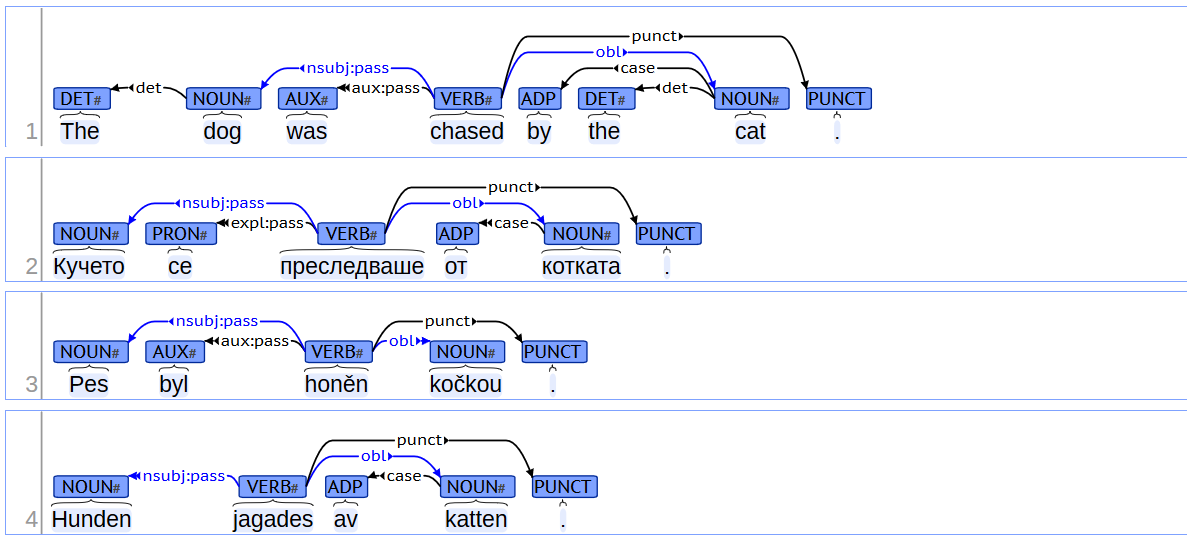
\includegraphics[width=1\textwidth]{images/ud_scheme.png}
	\caption{Ilustrace schéma UD anotace\cite{UDweb}}\label{fig:udscheme}
\end{figure}

\paragraph{CoNLL-U}
(nebo jednoduše Conllu) je textový formát pro zápis UD anotací\cite{UDweb}. Anotace jsou zakódované v prostém textu, čitelném jak strojově, tak i~pro člověka. Anotace každého slova/tokenu je na samostatném řádku. Řádky Conllu formátu jsou tří typů:
\begin{enumerate}
    \item řádek obsahující anotaci tokenu, která se skládá z 10 polí oddělených tabulátory,
    \item prázdný řádek, označující hranice vět,
    \item komentář, začínající znakem \#.
\end{enumerate}

Věty tvoří alespoň jedna řádka s tokenem, který obsahuje následující pole:
\begin{enumerate}
    \item ID: index ve větě,
    \item FORM: původní forma,
    \item LEMMA: lemma či stem,
    \item UPOS: univerzální \uv{part-of-speech} (dále POS) tag,
    \item XPOS: jazykově specifické POS tagy,
    \item FEATS: výčet morfologických vlastností,
    \item HEAD: předek v závislostním stromu,
    \item DEPREL: závislostní vazba k předkovi,
    \item DEPS: rozšířený závislostní graf,
    \item MISC: další anotace.
\end{enumerate}

% <příklad>
\begin{example}
Pro ukázku je na obrázku \ref{fig:conlluexample} vidět anotace vzorové věty.
    
\begin{figure}\centering
	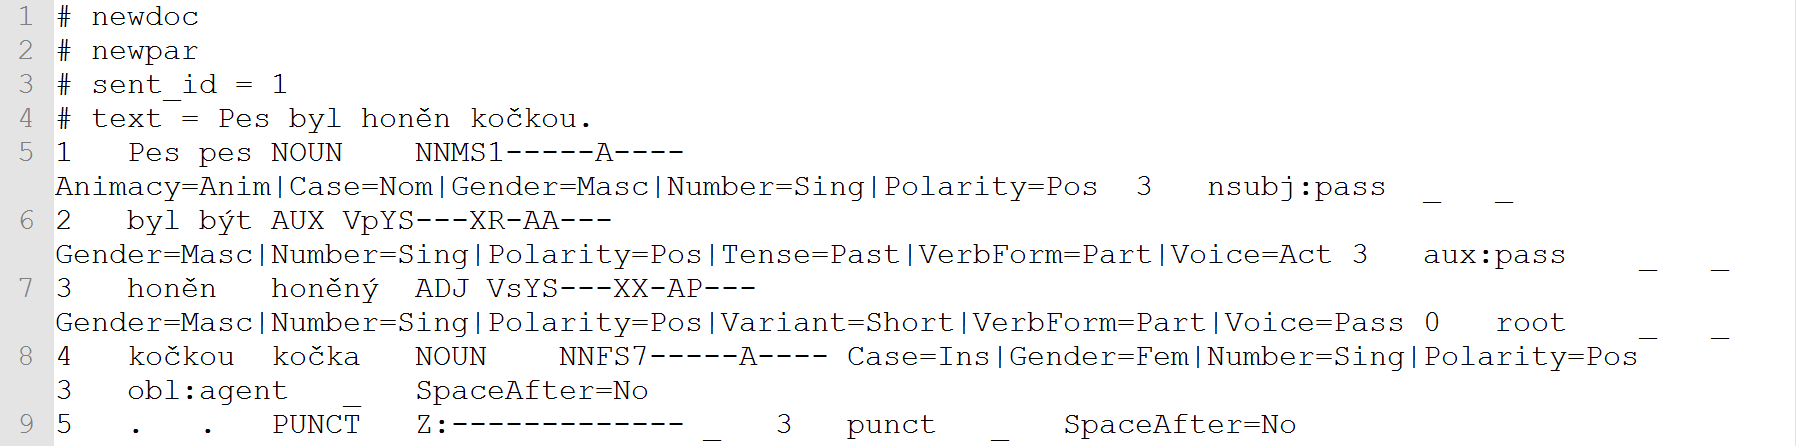
\includegraphics[width=1\textwidth]{images/conllu_example.PNG}
	\caption{Ukázka CoNLL-U formátu}\label{fig:conlluexample}
\end{figure}
\end{example}


\subsubsection{Nástroje pro práci s jazykem}

\paragraph{Treex}

je modulární NLP framework zaměřený na strojové překlady\cite{Treex}. Pomocí specifických modulů lze složit scénáře, například pro tektogramatickou analýzu na úrovni PDT. Je implementovaný v jazyku Perl a využít lze ve formě webového rozhraní. Současně je již nástroj zastaralý a nahrazují ho následující.

\paragraph{UDPipe}

je nástroj provádějící segmentizaci, tokenizaci, tagování, lematizaci a analýzu závislostí textu\cite{UDPipe}. Pomocí nástroje lze trénovat vlastní, nebo přímo využívat předtrénované UD modely. Standardně pracuje s CoNLL-U formátem. Je optimalizovaný pro rychlost. Je multiplatformní, podporuje rozhraní pro většinu populárních jazyků a lze ho využít i v podobě webové aplikace.

\paragraph{Udapi}

je rozraní a framework pro zpracovávání UD\cite{Udapi}. Je dostupný jako nástroj příkazové řádky, nebo knihovna pro jazyky Python, Perl a Java. Vnitřní reprezentace Conllu dat v Udapi je čtyřvrstvá hierarchická struktura skládající se z:
\begin{enumerate}
    \item dokumentů -- jednotlivé Conllu dokumenty,
    \item svazků -- (z angl. bundles) dokument může mít několik svazků, reprezentujících jednu větu dokumentu,
    \item stromů -- (z angl. trees) svazek může mít několik stromů, kde každý strom reprezentuje jazykovou mutaci dané věty odvozenou dle treebanky,
    \item uzlů -- (z angl. nodes) stromy se klasicky skládají z uzlů reprezentujících jednotlivá slova (tokeny).
\end{enumerate}

\paragraph{conllu}

je odlehčená knihovna pro jazyk Python umožňující základní operace s CoNLL-U daty.

\subsubsection{Výběr technologií a implementace}
\label{sec:subj_conllu_extraction}

Aktuální technologický trend vývoje NLP aplikací je u UD. Pro účely extrakce předmětných položek podle větného rozkladu vybírám model \textit{czech-pdt-ud-2.5-191206}\cite{UD_Czech-PDT}, který používám v nástroji \textit{UDPipe} pro anotaci textu a takto anotovaný text následně procesuji za použití \textit{Udapi}.

Proces extrakce podle větného rozkladu tak spočívá ve třech krocích:
\begin{enumerate}
    \item Anotace textu a převedení do vnitřní reprezentace
    
    Nejprve provádím anotaci pomocí \textit{UDPipe}, který souvislý text kontextu převede do \textit{Conllu} formátu (segmentace vět, tokenizace slov...). Následně tato data načítám do \textit{Udapi}, čímž získávám jejich vnitřní reprezentaci.
    
    \item Filtrování vnitřní reprezentace
    
    Filtrování provádím větu po větě, respektive strom po stromu (vzhledem k použití pouze jedné treebanky má svazek vždy jen jeden strom). Nejprve filtruji jednoduše na základě klíčových slov týkajících se nerelevantních informací jako jsou ceny nebo přílohy dokumentů tak, že odmažu celý podstrom těchto slov.
    
    Následuje hlavní krok filtrování, který na základě komplexních podmínek vybírá předmětné části. Více do detailu popisuji tento krok v samotné kapitole \ref{sec:nonsubj_parts_filter}
    
    
    \item Převedení zpět do textové podoby
    
    Nakonec převádím zbývající data z \textit{Udapi} reprezentace zpět do prostého textu.
    
\end{enumerate}

\subsubsection{Filtrování (ne)předmětných částí vět}
\label{sec:nonsubj_parts_filter}

% <příklad>
Pro úvod nejdříve uvedu příklad, na kterém nastíním myšlenku a proces tohoto filtru.

% \begin{example}
\begin{quote}
    Mějme větu: "Předmětem plnění této veřejné zakázky je dodávka zemědělských strojů.", jejíž rozklad je na obrázku \ref{fig:decompositionexample}. Předmětná část této věty je \uv{dodávka zemědělských strojů}. Otázkou je, jakým vzorem takovou část podchytit?
    
    Závislostní vazba uzlu \uv{dodávka} na předchůdce (\uv{předmětem}) je \textit{nsubj}. Zdá se, že by se v tom případě dalo odchytávat koncové uzly vazby \textit{nsubj} a jejich podstromy.
    
    \begin{figure}\centering
    	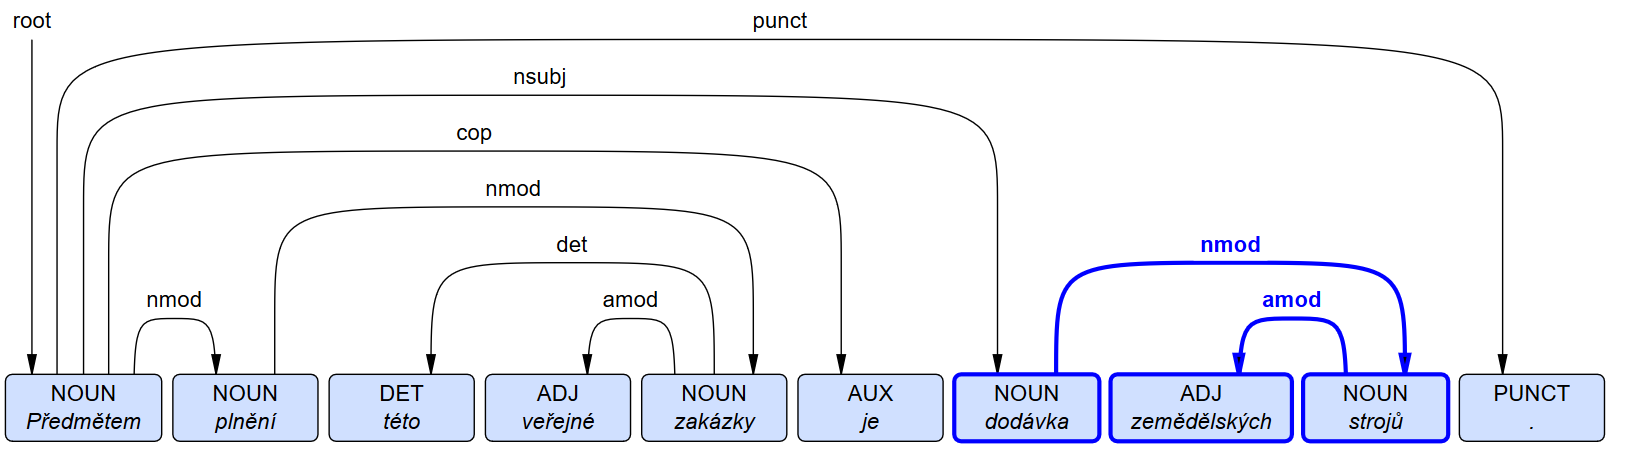
\includegraphics[width=1\textwidth]{images/decomposition_example.PNG}
    	\caption[Ukázka rozkladu předmětné věty]{Ukázka rozkladu předmětné věty (předmětná část věty je zvýrazněna modře)}\label{fig:decompositionexample}
    \end{figure}
\end{quote}
% \end{example}

Bohužel, ne vždy je situace takto přímočará. Treebanky jsou navíc omezeně rozsáhlé a dochází k chybám anotace, které jsou někdy kritické.

Obecně, algoritmus výběru části vět zakládám na selekci kandidátních uzlů a následném doplnění o jejich kontext.

\newpage
Selekce kandidátních uzlů je řízena následujícími podmínkami:
\begin{itemize}
    \item vyhovující závislostní vazby (větné členy) omezuji na\footnote{Jednotlivé definice vazeb jsou dostupné v angličtině v dokumentaci UD\cite{UDweb}.}:
    % \begin{table}
    % \centering
    % \begin{tabular}{ |l|l|l|l| }
    % \hline
    % Název vazby & Větný člen & Anglické znění & obrázek\\\hline
    % \multicolumn{4}{|l|}{Příklad} \\\hline
    % \hline
    % \textit{nsubj} & podmět & nominal subject & \ref{fig:nsubjexample}\\\hline
    % \multicolumn{4}{|l|}{Předmětem jsou zemědělské \textbf{stroje}.} \\\hline
    % \hline
    % \textit{nsubj:pass} & pasivní podmět & passive nominal subject & \ref{fig:nsubjpassexample}\\\hline
    % \multicolumn{4}{|l|}{Dodavatelem budou dodány zemědělské \textbf{stroje}.} \\\hline
    % \hline
    % \textit{obj} & předmět & direct object & \ref{fig:objexample}\\\hline
    % \multicolumn{4}{|l|}{Dodavatel dodá zemědělské \textbf{stroje}.} \\\hline
    % \hline
    % \end{tabular}
    % \caption{Měření dopadu jednotlivých extraktorů (podle lokálních charakteristik) na dopad extrakce předmětných položek}
    % \label{table:experiment_extractors1}
    % \end{table}
    \begin{itemize}
        \item \textit{nsubj} (podmět; z angl. \uv{nominal subject})\newline
        např. "Předmětem jsou zemědělské \textbf{stroje}."\newline
        (viz. obrázek \ref{fig:nsubjexample}),
        \item \textit{nsubj:pass} (pasivní podmět; z angl. \uv{passive nominal subject})\newline
        např. "Dodavatelem budou dodány zemědělské \textbf{stroje}."\newline
        (viz. obrázek \ref{fig:nsubjpassexample}),
        \item \textit{obj} (předmět; z angl. \uv{direct object})\newline
        např. "Dodavatel dodá zemědělské \textbf{stroje}."\newline
        (viz. obrázek \ref{fig:objexample}),
        \item \textit{obl} (doplněk; z angl. \uv{oblique argument or adjunct})\newline
        např. "Dodavatel se zavazuje k \textbf{dodání} zemědělských strojů."\newline
        (viz. obrázek \ref{fig:oblexample}),
        \item \textit{obl:arg} (předmět; z angl. \uv{oblique argument})\newline
        např. "Předmět spočívá v \textbf{dodání} zemědělských strojů."\newline
        (viz. obrázek \ref{fig:oblargexample}),
        \item \textit{nmod} (přívlastek neshodný; z angl. \uv{nominal modifier})\newline
        např. "Předmětem je \textbf{dodání} zemědělských strojů."\newline
        (viz. obrázek \ref{fig:nmodexample}).
    \end{itemize}
    \item specifikuji množinu zakázaných slov v podobě lemat (např. \textit{smlouva, předmět, specifikace, dokumentace, uzavření, dodatek, podmínka...}),
    \item podobně specifikuji množinu zakázaných slov, které nesmějí předcházet (např. \textit{dodatečný, nutný...}),
    \item nakonec specifikuji slovesa, která by měla předcházet (např. \textit{zavazovat, dodat, zajistit, provést...}).
\end{itemize}

% http://lindat.mff.cuni.cz/services/udpipe/
% https://urd2.let.rug.nl/~kleiweg/conllu/
\begin{figure}\centering
	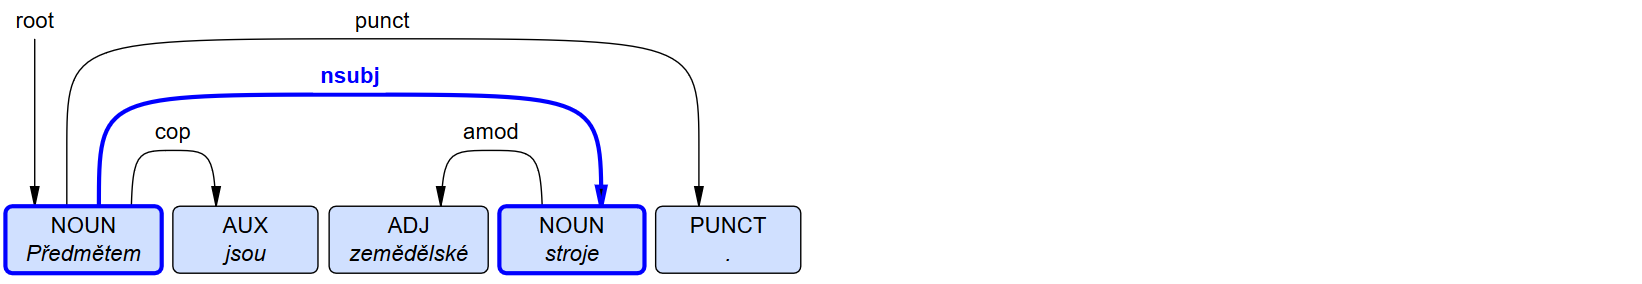
\includegraphics[width=1\textwidth]{images/nsubj_example.png}
	\caption{Ukázka předmětné části jako vazby \textit{nsubj}}\label{fig:nsubjexample}
\end{figure}

\begin{figure}\centering
	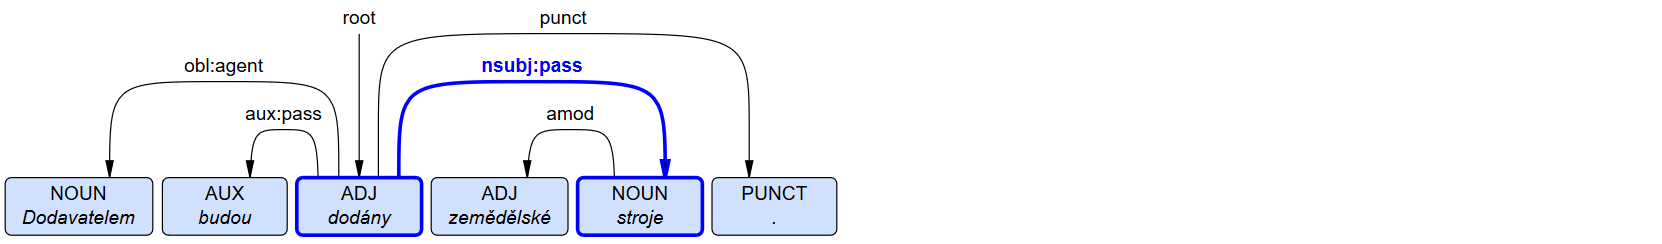
\includegraphics[width=1\textwidth]{images/nsubjpass_example.png}
	\caption{Ukázka předmětné části jako vazby \textit{nsubj:pass}}\label{fig:nsubjpassexample}
\end{figure}

\begin{figure}\centering
	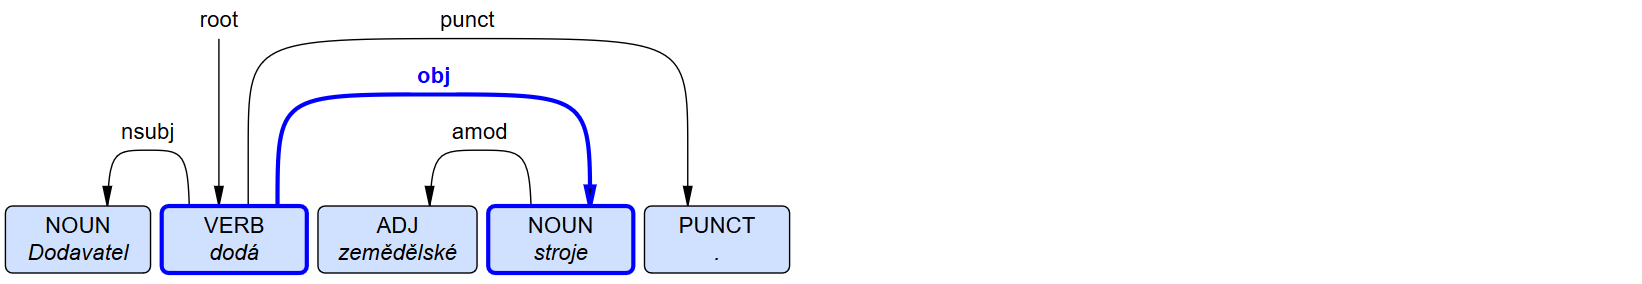
\includegraphics[width=1\textwidth]{images/obj_example.png}
	\caption{Ukázka předmětné části jako vazby \textit{obj}}\label{fig:objexample}
\end{figure}
\begin{figure}\centering
	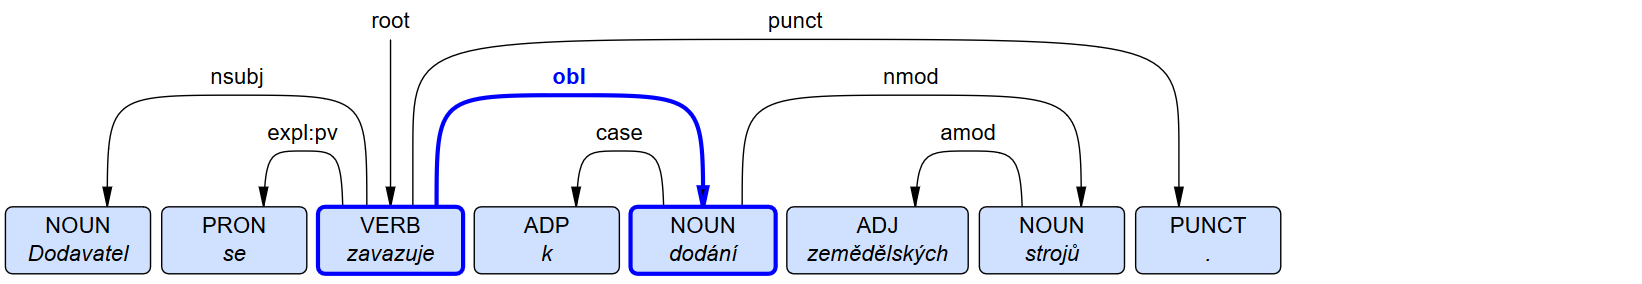
\includegraphics[width=1\textwidth]{images/obl_example.png}
	\caption{Ukázka předmětné části jako vazby \textit{obl}}\label{fig:oblexample}
\end{figure}
\begin{figure}\centering
	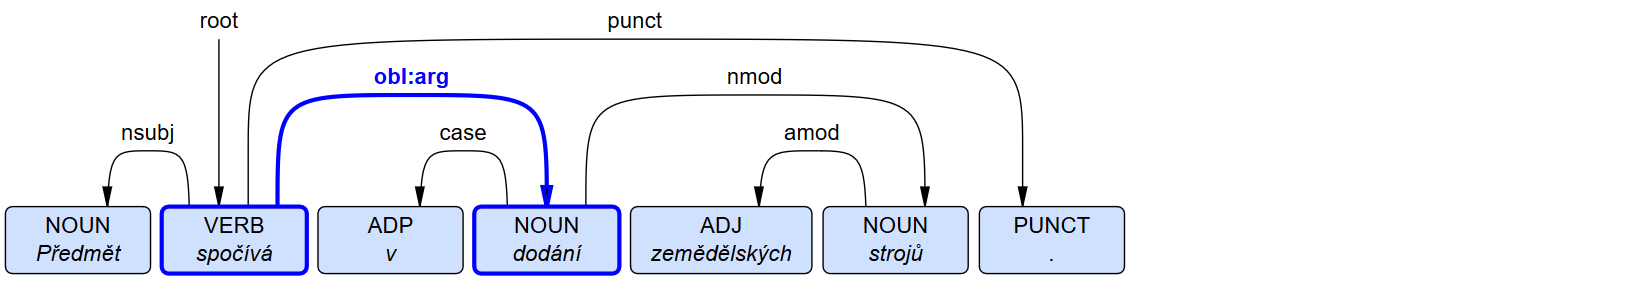
\includegraphics[width=1\textwidth]{images/oblarg_example.png}
	\caption{Ukázka předmětné části jako vazby \textit{obl:arg}}\label{fig:oblargexample}
\end{figure}
\begin{figure}\centering
	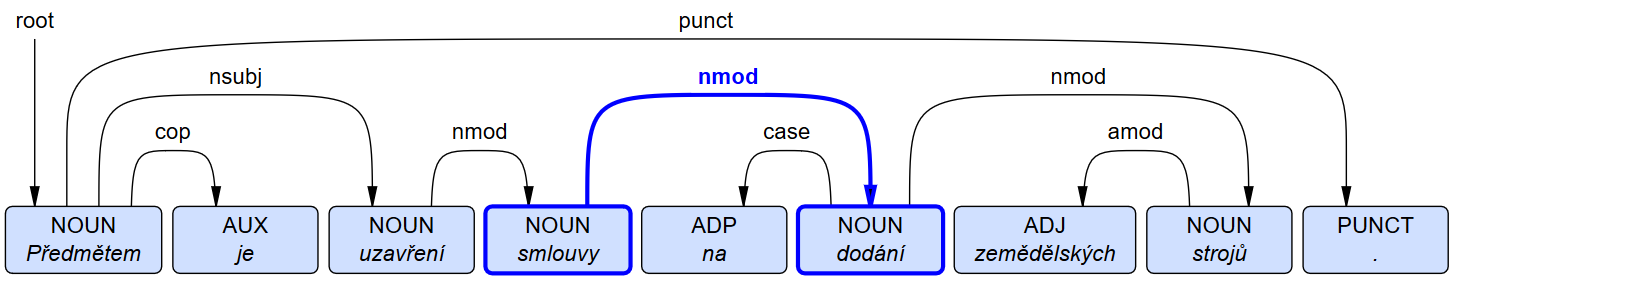
\includegraphics[width=1\textwidth]{images/nmod_example.png}
	\caption{Ukázka předmětné části jako vazby \textit{nmod}}\label{fig:nmodexample}
\end{figure}



Pokud je ve větě více cílových kandidátních slov v konjunktivním vztahu (\textit{conj}), předchozí selekce vybere často pouze první z nich. Proto každé kandidátní slovo rozšiřuji o jeho konjunktivní doplněk.

Takto vybraná kandidátní slova rozšiřuji o jejich kontext pro výběr celé části věty. Kontext obvykle vybírám jako podstrom daného kandidátního slova. Celé vybrané části ještě dodatečně filtruji vzhledem k různým vlastnostem, aby například netvořily příliš dlouhé řetězce. Jako vyfiltrovaný výstup pro danou větu spojuji všechny takto vybrané části.

\subsection{Sestavení komponenty pro extrakci předmětu}

Komponentu pro extrakci předmětu sestavuji podle návrhu celého procesu (viz. \ref{sec:subj_extraction_design}) tak, že provádí kroky:
\begin{enumerate}
    \item Identifikace a extrakce kontextů předmětu (\ref{sec:subj_context_identification})
    \item Předzpracování jednotlivých kontextů na základě lokálních charakteristik (\ref{sec:subj_filtering})
    \item Extrakce položek z předzpracovaného kontextu
    (\ref{sec:local_stats_extraction})
    \item Anotace vyfiltrovaného kontextu (\ref{sec:subj_conllu_extraction})
    \item Filtrování anotovaného kontextu podle větného rozkladu (\ref{sec:nonsubj_parts_filter})
    \item Extrakce zbylých položek vyfiltrovaného anotovaného kontextu
    \item Sloučení obou skupin položek
\end{enumerate}

Komponenta přijímá jakýkoli souvislý text a vrací formátovaný text obsahující odřádkované jednotlivé položky.
\newpage

\section{Extrakce lokality a předmětu podnikání zadavatelů}
\label{sec:locality&subsub_extraction}

V kapitolách \uv{Data o lokacích}(\ref{sec:data_locality}) a \uv{Data o předmětu podnikání zadavatelů}(\ref{sec:data_subsub}) uvádím možnost získání informací o lokalitě a předmětu podnikání zadavatelů zakázek.

Na základě toho implementuji komponentu, která pro jednotlivé zadavatele posílá dotaz podle čísla IČO na rozhraní systému ARES pro získání informací o daném zadavateli. Z odpovědi komponenta extrahuje oboje adresu i předmět podnikání.

Pro další zpracování adresy implementuji geokodér spočívající v dotazování se na službu geokódování portálu Mapy.cz.

Získaný předmět podnikání rozděluji podle odřádkování do jednotlivých položek.


\chapter{Metrika podobnosti zakázek}

Jednou z nezbytných částí doporučovacích systémů je metrika podobnosti položek, které systém doporučuje. Správně zvolená/navržená metrika musí reflektovat důležité vlastnosti porovnávaných položek, avšak tyto vlastnosti se mohou lišit v závislosti na úloze. Žádná metrika není univerzálně použitelná ve všech případech. 

V doméně veřejných zakázek se můžeme ptát na otázku: jaké zakázky jsou si podobné? Pro účely mé práce definuji následující vlastnosti pro určení takové podobnosti: předmět plnění zakázky, lokalita zadavatele a předmět podnikání zadavatele.

Zatímco podobnost lokality zadavatele lze intuitivně řešit přímo jako inverzní funkce geografické vzdálenosti dvou bodů (např. podle sídla zadavatele), předmět podnikání zadavatele a samotný předmět plnění zakázky již takto přímo měřit nelze. Podobnost předmětu zakázek by mohla jít řešit na základě CPV kódů, avšak jen do omezeného rozsahu jejich hierarchické struktury. Pro obecné řešení se tak nabízí řešení podobnosti předmětu specifikovaného v textu dokumentace zakázek.

\newpage
\section{Metrika podobnosti textu}
\label{sec:text_sim_metrics}

Existuje mnoho algoritmů pro porovnávání textových řetězců. Podle základní myšlenky se člení na algoritmy založené na\cite{mayank2019}:

\begin{enumerate}
    \item editační vzdálenosti
    
    Metoda spočívá v počítání operací nutných pro transformaci jednoho řetězce na druhý. Čím více je potřeba operací, tím méně jsou si řetězce podobné.
    
    Příkladem jsou algoritmy Hammingovy či Levenshteinovy vzdálenosti.

    \item množinových operacích
    
    Algoritmy této kategorie dělí řetězce na množiny tokenů a hledají se podobné tokeny z obou množin. Čím více podobných tokenů množiny mají, tím jsou si samotné řetězce více podobné.
    
    Zástupcem této metody je tvz. \uv{Jaccard index}, který používám při validacích algoritmů pracujících s textem. Tento index udává podobnost dvou množin jako podíl jejich průniku se součinem, viz. předpis \ref{eq:jaccard}.
    \begin{equation} \label{eq:jaccard}
    J(A,B) := \frac{|A \cap B|}{|A \cup B|}
    \end{equation}
    
    \item hledání společných sekvencí
    
    U této kategorie spočívá metrika v hledání společných sekvencí obou řetězců.
    
    Například algoritmus Ratcliff-Obershelpovy vzdálenosti využívá binární dělení a hledání nejdelších podřetězců v obou větvích.
    
\end{enumerate}

Všechny tyto algoritmy jsou zaměřené pouze na podobnosti řetězců samotných, což je postačující v případech, kdy jsou si tyto řetězce poměrně podobné. To nastává například při validaci výsledků transformace textu oproti referenční hodnotě.

V případě, kdy je potřeba řešit významová (sémantická) podobnost textů však tyto metody selhávají. Sémantická podobnost textů je netriviální problém sám o sobě, dnes běžně řešený za pomocí modelů strojového učení. U řešení sémantické podobnosti se hlavní problém přenáší na transformaci obsahu textu do prostoru vlastností (vektorového prostoru), ve kterém lze vzdálenost (podobnost, souvislost) měřit. Příkladem takové transformace je proces tzv. \uv{embeddingu} dokumentů, který detailně popisuji v samotné kapitole \ref{sec:document_embedding}.

Pro měření vzdálenosti dokumentů převedených do vektorového prostoru je vhodná kosinová vzdálenost, jak popisuje do detailu ve svém článku\cite{emmery2017} Emmery. Oproti euklidovské vzdálenosti kosinová vzdálenost potlačuje odchylky způsobené absolutní délkou textů.

\newpage
\section{Komponenty pro vyhodnocování podobnosti}

\subsection{Výpočet Jaccard indexu}
\label{sec:component_jaccard_index}

Komponenta využívá knihovny \textit{textdistance}\footnote{textdistance - Python knihovna; dostupná z https://pypi.org/project/textdistance/}, která poskytuje všechny algoritmy zmíněné v kapitole \ref{sec:text_sim_metrics} a mnoho dalších. Knihovní funkce přijímá dvě kolekce tokenů a vrací jejich podobnostní index. Tokenizaci obou řetězců provádím jednoduše rozdělováním podle mezer. Knihovna pracuje s množinami jako s tzv. multimnožinami, tedy bere v úvahu počty výskytů.
    
\subsection{Výpočet geografické podobnosti}
\label{sec:component_geospatial_similarity}
    
Komponenta počítá vzdálenost mezi cílovým a referenčním GPS bodem a následně odvozuje jejich \uv{podobnost}. Pro výpočet vzdálenosti (geodezické\footnote{Geodezická vzdálenost - vzdálenost po povrchu Země jako elipsoidu}) využívám knihovny \textit{geopy}\footnote{geopy - Python knihovna; dostupná z https://pypi.org/project/geopy/}, která -- mimo jiné -- poskytuje různé algoritmy počítání geografické vzdálenosti. Knihovní funkce přijímá dva GPS body a vrací metrickou vzdálenost. Vzdálenost v kilometrech převádím na podobnost standardizací danou předpisem \ref{eq:log1p_standardization}, kde \textit{d} je vypočítaná nenulová vzdálenost a \textit{log1p} je speciální logaritmická funkce knihovny \textit{numpy}, definovaná jako přirozený logaritmus z \textit{x+1}.
\begin{equation} \label{eq:log1p_standardization}
Sim(d) := min(1, \frac{1}{log1p(d)})
\end{equation}
Tato standardizace má za důsledek, že vzdálenosti do 1,7 kilometru dávají podobnost 1, což zhruba odpovídá logické podobnosti na úrovni stejné obce, jako je znázorněno v diagramu \ref{fig:log1pstandardization}.
\begin{figure}\centering
	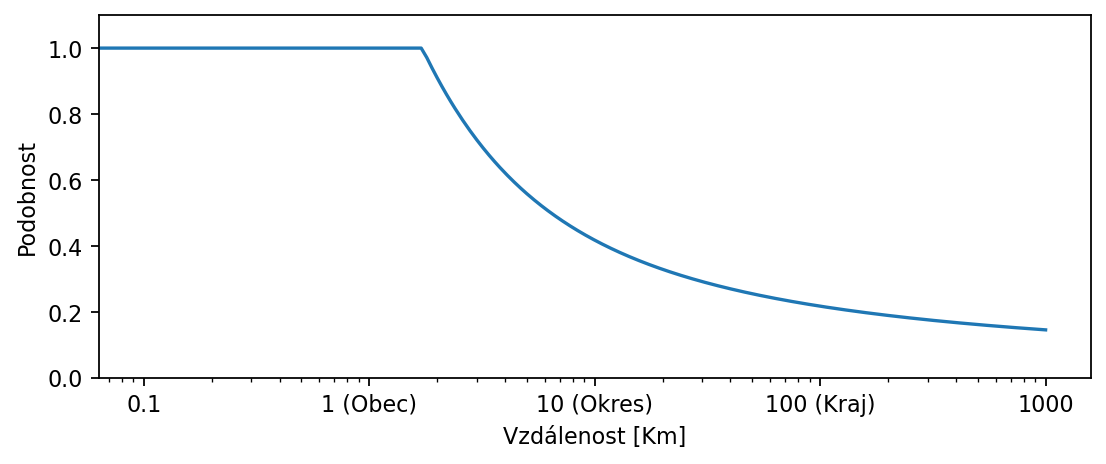
\includegraphics[width=0.9\textwidth]{images/log1p_standardization.png}
	\caption{Ukázka průběhu geografické podobnosti \ref{eq:log1p_standardization}}\label{fig:log1pstandardization}
\end{figure}

Komponenta přijímá na vstupu tvz. \uv{\textit{pandas}\footnote{pandas - Python knihovna; dostupná z https://pypi.org/project/pandas/} dataframe} pro cílovou a referenční množinu bodů a na výstupu vrací mapu \textit{n} nejbližších referenčních bodů pro každý z cílových.
    
\subsection{Výpočet kosinové podobnosti}
\label{sec:component_cosine_similarity}

Komponenta, obdobně jako předchozí, počítá vzdálenost mezi cílovým a referenčním bodem (vektorem) a následně odvozuje jejich \uv{podobnost}.
Pro výpočet (kosinové) vzdálenosti vektorů podle definice \ref{eq:cosine_distance} implementuji komponentu založenou na maticových operacích pomocí nástrojů knihovny \textit{numpy}.
Komponenta  přijímá dvě kolekce vektorů a vrací kosinovou vzdálenost všech párů vektorů mezi těmito dvěma kolekcemi.
Komponenta vrací vzdálenost v intervalu \interval[0,2], kterou převádím na podobnost standardizací danou předpisem \ref{eq:cosine_standardization}, kde \textit{d} je vypočítaná vzdálenost.

\begin{equation} \label{eq:cosine_distance}
CosDist(\mathbf{A}, \mathbf{B}) := 1 - \frac{\mathbf{A} \cdot \mathbf{B}}{\| \mathbf{A}\|*\| \mathbf{B}\|}
\end{equation}

\begin{equation} \label{eq:cosine_standardization}
Sim(d) := \frac{2-d}{2}
\end{equation}

\begin{quote}
    Pro výpočet kosinové vzdálenosti nepoužívám knihovní funkce z důvodu optimalizace výpočtu pomocí částečného předpočítání matic působících ve výpočtu. Výsledek optimalizace je zaznamenaný v tabulce \ref{table:experiment_similarity}. Měření je prováděno na kolekcích 100 cílových vektorů (měnících se) oproti 10\,000 referenčních vektorů (stálých) o dimenzi 300. Výpočty jsou prováděny ve 100 epochách pro podchycení amortizační optimalizace předpočítání stálých matic.
\end{quote}
\begin{table}[h!]
\centering
\begin{tabular}{ |l|l|r| }
\hline
Knihovna & Funkce & Čas [s] \\\hline
\hline
\textit{Sklearn}\footnotemark & \textit{cosine\_similarity} & 5.86 \\
\textit{SciPy}\footnotemark & \textit{cdist[cosine]} & 44.50 \\
--- & vlastní & 4.26 \\\hline
\end{tabular}
\caption{Měření doby výpočtu algoritmů pro výpočet kosinové vzdálenosti}
\label{table:experiment_similarity}
\end{table}
\footnotetext[33]{Sklearn (scikit--learn) -- Python modul pro strojové učení; dostupný z https://pypi.org/project/scikit-learn/}
\footnotetext[34]{SciPy -- Python knihovna pro matematické, vědecké a inženýrské úlohy; dostupná z https://pypi.org/project/scipy/}
\newpage

\subsection{Výpočet \uv{euklidovské} podobnosti}
\label{sec:component_euclidean_similarity}

\begin{quote}
Přestože pojem \uv{euklidovské podobnosti} není přesně definován, euklidovská vzdálenost (jinak zvaná jako euklidovská metrika) je obecně známý pojem a lze ji různými způsoby na podobnost převést.
\end{quote}

Oproti předešlé metodě tato komponenta počítá (euklidovskou) vzdálenost vektorů pomocí funkce \textit{euclidean\_distances} knihovny \textit{Sklearn}. Knihovní funkce přijímá dvě kolekce vektorů a vrací euklidovskou vzdálenost všech párů vektorů mezi těmito dvěma kolekcemi. Euklidovská vzdálenost nabírá oboru hodnot kladných reálných čísel a proto ji na podobnost převádím jednoduchou inverzní transformací podle předpisu
\ref{eq:euclidean_standardization}.
\begin{equation} \label{eq:euclidean_standardization}
Sim(d) := \frac{1}{d}
\end{equation}

\begin{quote}
    Podobně jako pro kosinovou vzdálenost se pokouším implementovat optimalizaci výpočtu euklidovské vzdálenosti na základě vztahu \ref{eq:euclidean_distance}\cite{dey2016}. Výsledek je ovšem neúspěšný, jak je zaznamenáno v tabulce \ref{table:experiment_similarity2}.
\end{quote}
\begin{equation} \label{eq:euclidean_distance}
EucDist(\mathbf{A}, \mathbf{B}) := \|\mathbf{A} - \mathbf{B}\|^2 = -2\mathbf{a}\mathbf{b} + \mathbf{a}\mathbf{a}^T + \mathbf{b}\mathbf{b}^T
\end{equation}
\begin{table}[h!]
\centering
\begin{tabular}{ |l|l|r| }
\hline
Knihovna & Funkce & Čas [s] \\\hline
\hline
\textit{Sklearn} & \textit{euclidean\_distances} & 4.06 \\
\textit{SciPy} & \textit{cdist[euclidean]} & 44.70 \\
--- & vlastní & 4.75 \\\hline
\end{tabular}
\caption{Měření doby výpočtu algoritmů pro výpočet euklidovské vzdálenosti}
\label{table:experiment_similarity2}
\end{table}


\chapter{Doporučovací systém}

V dnešní době je na internetu nepřeberné množství informací, zdrojů, věcí a~mnoho dalšího. K efektivnímu využití takového obsahu je zapotřebí systémů, které uživateli budou schopny data třídit do rozumně rozsáhlé množiny relevantních položek. Takové systémy se nazývají \uv{doporučovací} a vyskytují se v~podstatě ve všech populárních on-line platformách jako jsou Youtube, Amazon, Netflix, Facebook a mnoho dalších.

Jak shrnuje ve svém článku\cite{rocca2019} autor, ke stavbě doporučovacích systémů se používají dvě základní paradigma: tzv. \uv{kolaborativní filtrování} (dále angl. collaborative filtering) a \uv{obsahově založené} metody (dále angl. content-based).

\newpage
\section{Paradigma doporučovacích systémů}
\subsection{Collaborative filtering}

Metody kolaborativního filtrování jsou založené výhradně na předešlých interakcích uživatele s položkami systému. Interakce systém zaznamenává do tzv. \uv{uživatel--položka matice}(z angl. user--item matrix), na základě které systém zároveň detekuje podobné uživatele či položky.

Existují dvě základní kategorie algoritmů:
\begin{enumerate}
    \item Memory based
    
    Tzv. \uv{memory based} algoritmy jsou založené na přímém využití matice pro výpočet nejpodobnějších záznamů.
    
    \item Model based
    
    Metody tzv. \uv{model based} přístupu oproti tomu využívají odvozeného modelu, který zobecňuje zaznamenané interakce a snaží se v nich nalézt relevantní informaci pro provádění predikce.
    
\end{enumerate}

Výhoda kolaborativního filtrování je, že neklade žádné nároky na vstupní informace o uživatelích nebo položkách. Zároveň jsou nativně schopny efektivitu doporučování zlepšovat v průběhu fungování s přibývajícím počtem zaznamenaných interakcí.

Tato vlastnost ovšem přináší i jejich hlavní problém tzv. \uv{chladného startu} (z angl. cold start problem), který představuje situaci, že novému uživateli nelze nic doporučovat, stejně jako nelze doporučovat právě přidané položky. Existují různá řešení tohoto problému, mezi která patří například i použití nekolaborativní metody.

\subsection{Content based}
\label{sec:contentbased}

Jak napovídá název, metody tohoto typu jsou založené na obsahu, respektive vlastností obou uživatelů i položek, na základě kterých se staví model. Podle toho, které vlastnosti se využívají dělíme dva přístupy:
\begin{enumerate}
    \item Item--centered
    
    Tzv. \uv{item--centered} přístup využívá uživatelských vlastností pro predikci relevance dané položky ke všem uživatelům.
    
    \item User--centered
    
    \uv{User--centered} přístup naopak používá vlastnosti položek pro predikci jejich relevance pro daného uživatele.
    
\end{enumerate}

Metody obou přístupů lze zkombinovat tak, že se pro sestavení modelu využívají vlastnosti obou entit.

\subsection{Vyhodnocování doporučovacích systémů}
\label{sec:recommender_evaluation}

Vyhodnocování doporučovacích systémů je poněkud složité, přestože lze do určité míry použít standardní metody vyhodnocování algoritmů strojového učení. V případě, že je doporučovací model učený na množině zaznamenaných interakcí, lze použít klasických metrik chybovosti či přesnosti pro jeho automatické vyhodnocování.

U doporučování hraje důležitou roli vyrovnaný poměr explorace a exploatace. Kromě pouhého získání nejbližšího výsledku nás tak zajímá i jeho různorodost. Na důvěryhodnost systému má také dopad vysvětlitelnost jednotlivých doporučení. Takové, a jiné vlastnosti je možné vyhodnocovat za běhu systému při zaznamenávání reálného chování uživatelů na jednotlivé doporučené položky.
\newpage

\section{Návrh doporučovacího algoritmu}
\label{sec:recommender_design}

\begin{quote}
    V kapitole často používám pojmenování \uv{cílová} či \uv{referenční} matice, vektor, položky apod. Pojmem \uv{cílová} označuji entitu, na základě které systém dohledává entity \uv{referenční}. Například tak může vzniknout cílový dotaz obsahující cílovou položku \uv{zemědělské stroje}, která se převádí do reprezantace cílového vektoru či matice. Dotaz se dotazuje oproti referenčním položkám v referenčním datasetu (databázi), které se taktéž převádí do reprezentace referenčních vektorů respektive matice.
\end{quote}

Vzhledem ke zmíněnému problému chladného startu kolaborativních metod, který by v doméně veřejných zakázek měl kritický dopad volím pro doporučovací algoritmus metodu založenou na obsahu (viz. kapitola \ref{sec:contentbased}).

Povaha uživatelů (zadavatelů) a položek (zakázek) je do značné míry související ve smyslu podobnosti předmětu zakázek s předmětem podnikání zadavatelů či místnímu zařazení obou entit. Návrh algoritmu tak zakládám na všech těchto podobnostech zkombinováním vlastností obou uživatelů i položek.

Algoritmus je navržený pro zpracování obecného cílového dotazu na referenční dataset. Dotaz může být zadán jak ve smyslu konkrétního vyhledávání, tak ve smyslu doporučování na základě uživatelského (preferenčního) profilu. Skládání obou cílového dotazu a referenčního datasetu na základě patřičných vlastností je zobrazeno na schéma \ref{fig:recommenderfeatures}. Vlastnosti jsou reprezentované jednotlivými barvami.

Uživatelský profil se skládá ze zájmových položek a lokality uživatele. Profil může být inicializován na základě údajů zadavatele identifikovaného podle čísla IČO, nebo zadán ručně uživatelem, jak je zobrazeno na schéma \ref{fig:recommenderfeatures}.

\begin{figure}\centering
	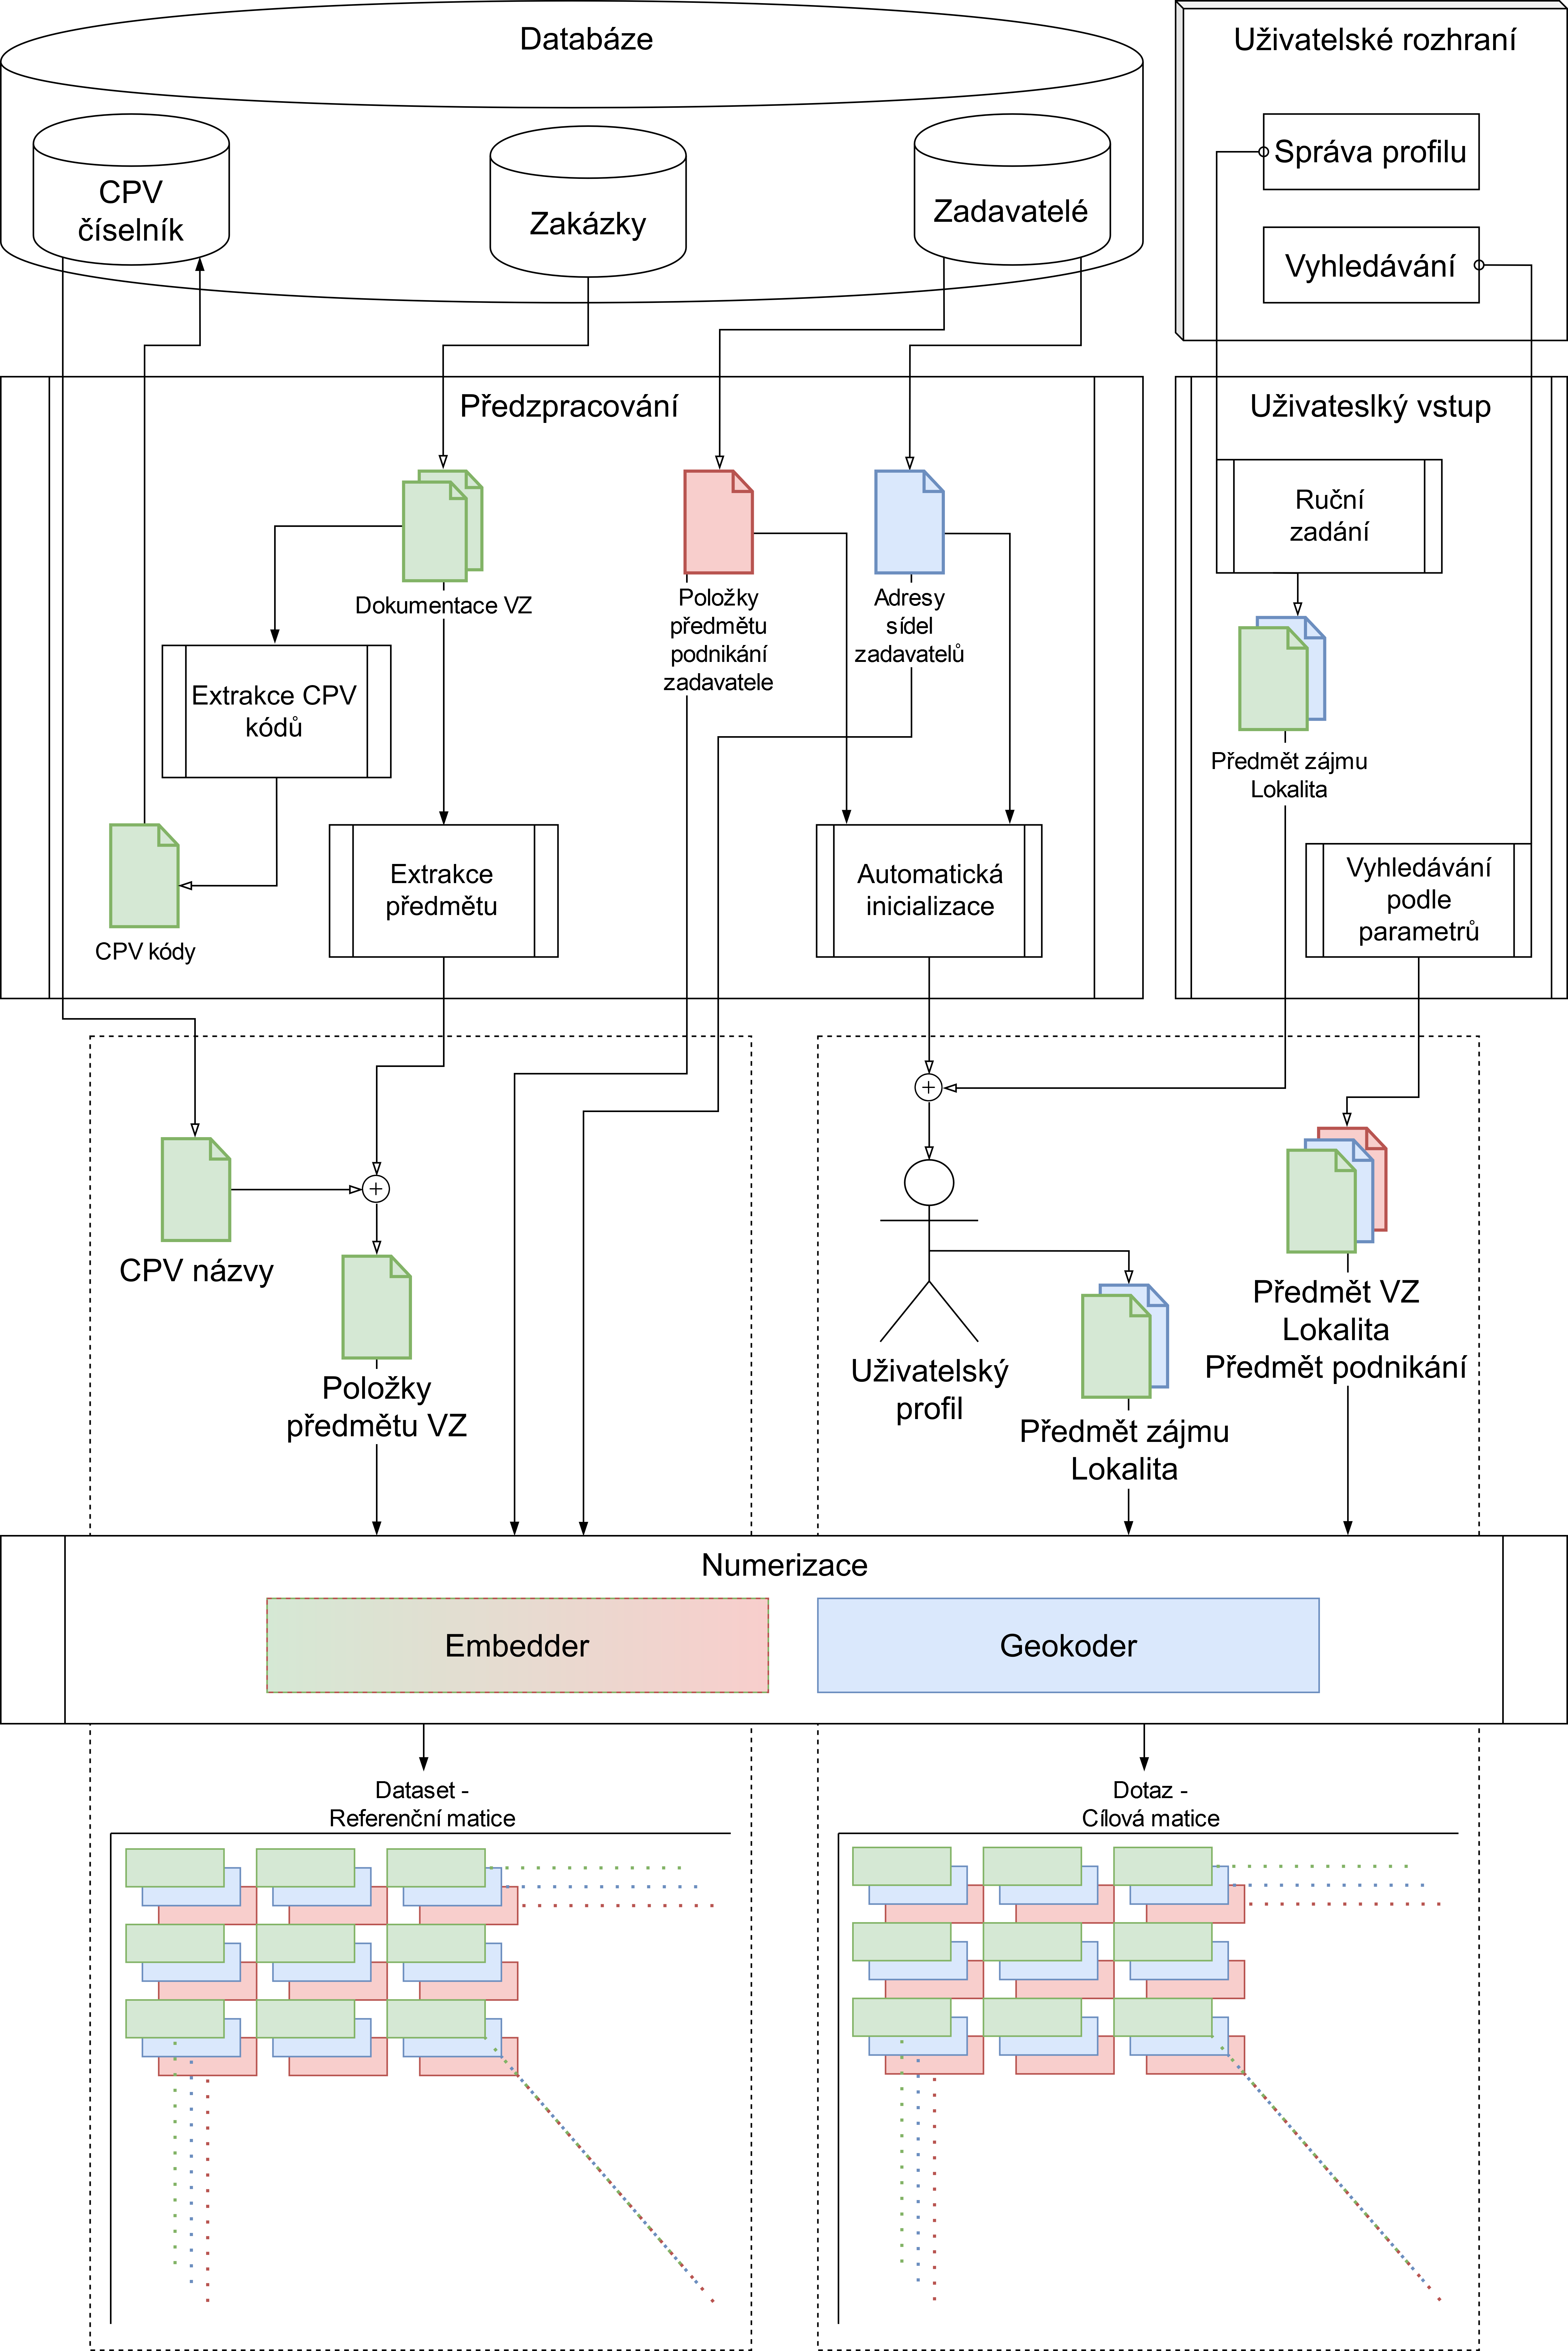
\includegraphics[width=1\textwidth]{images/recommender_features.png}
	\caption[Schéma skládání vlastností pro cílový dotaz a referenční dataset]{Schéma skládání vlastností pro cílový dotaz a referenční dataset. Jednotlivé vlastnosti jsou reprezentované barvami: zelená -- předmět, červená -- předmět podnikání zadavatele, modrá -- lokalita.}\label{fig:recommenderfeatures}
\end{figure}

Před samotným započetím operace výpočtu podobnosti jsou všechny vlastnosti numerizovány.

Celý algoritmus doporučování se skládá z jednotlivých komponent, kde každá se zaměřuje na určitou vlastnost. Jednotlivé komponenty lze využít samostatně, nebo je libovolně kombinovat s různými váhami.

V následujících kapitolách popisuji jednotlivé komponenty podle vlastnosti, na kterou se zaměřují.
\newpage

\subsection{Předmět zakázky}
\label{sec:feature_subject}

Předmět zakázky je hlavní vlastnost, na základě které je celý systém postaven. V kapitole \ref{sec:subjextraction} popisuji dopodrobna způsob extrakce předmětu zakázek do podoby jednotlivých položek. Na schématech \ref{fig:recommenderfeatures} a \ref{fig:recommender_algorithm} je reprezentovaná zelenou barvou.

Kromě samotných položek předmětu extrahuji i CPV kódy, jak popisuji v kapitole \ref{sec:cpv_extraction}. Názvy těchto kódů využívám jako dodatečné položky předmětu.

Každá položka je embeddovaná pomocí embedderu (kap. \ref{sec:component_embedding}) do vektorové reprezentace, ve které ji dále používám ve smyslu referenčního vektoru komponentou pro výpočet vektorové podobnosti (kap. \ref{sec:component_cosine_similarity}).

Na předměty jednotlivých zakázek v podobě referenčních vektorů sestavuji dotaz ve stejné reprezentaci cílových vektorů složený z:
\begin{enumerate}
    \item jedné či více položek přímého vyhledávání,
    \item zájmových položek uživatelského profilu.
\end{enumerate}

Komponenta výpočtu vektorové podobnosti vrací jako výsledek matici podobnosti cílových položek dotazu vůči referenčním položkám zakázek. Tyto podobnosti agreguji váženým průměrem podle jednotlivých zakázek, kde váhy položek jsou podobnosti samy o sobě (pro umocnění podobnějších položek oproti nepodobným). Touto agregací získávám relevanci zakázky podle jejího předmětu, jako je zobrazeno na schéma
\ref{fig:recommender_algorithm}.

\begin{figure}\centering
	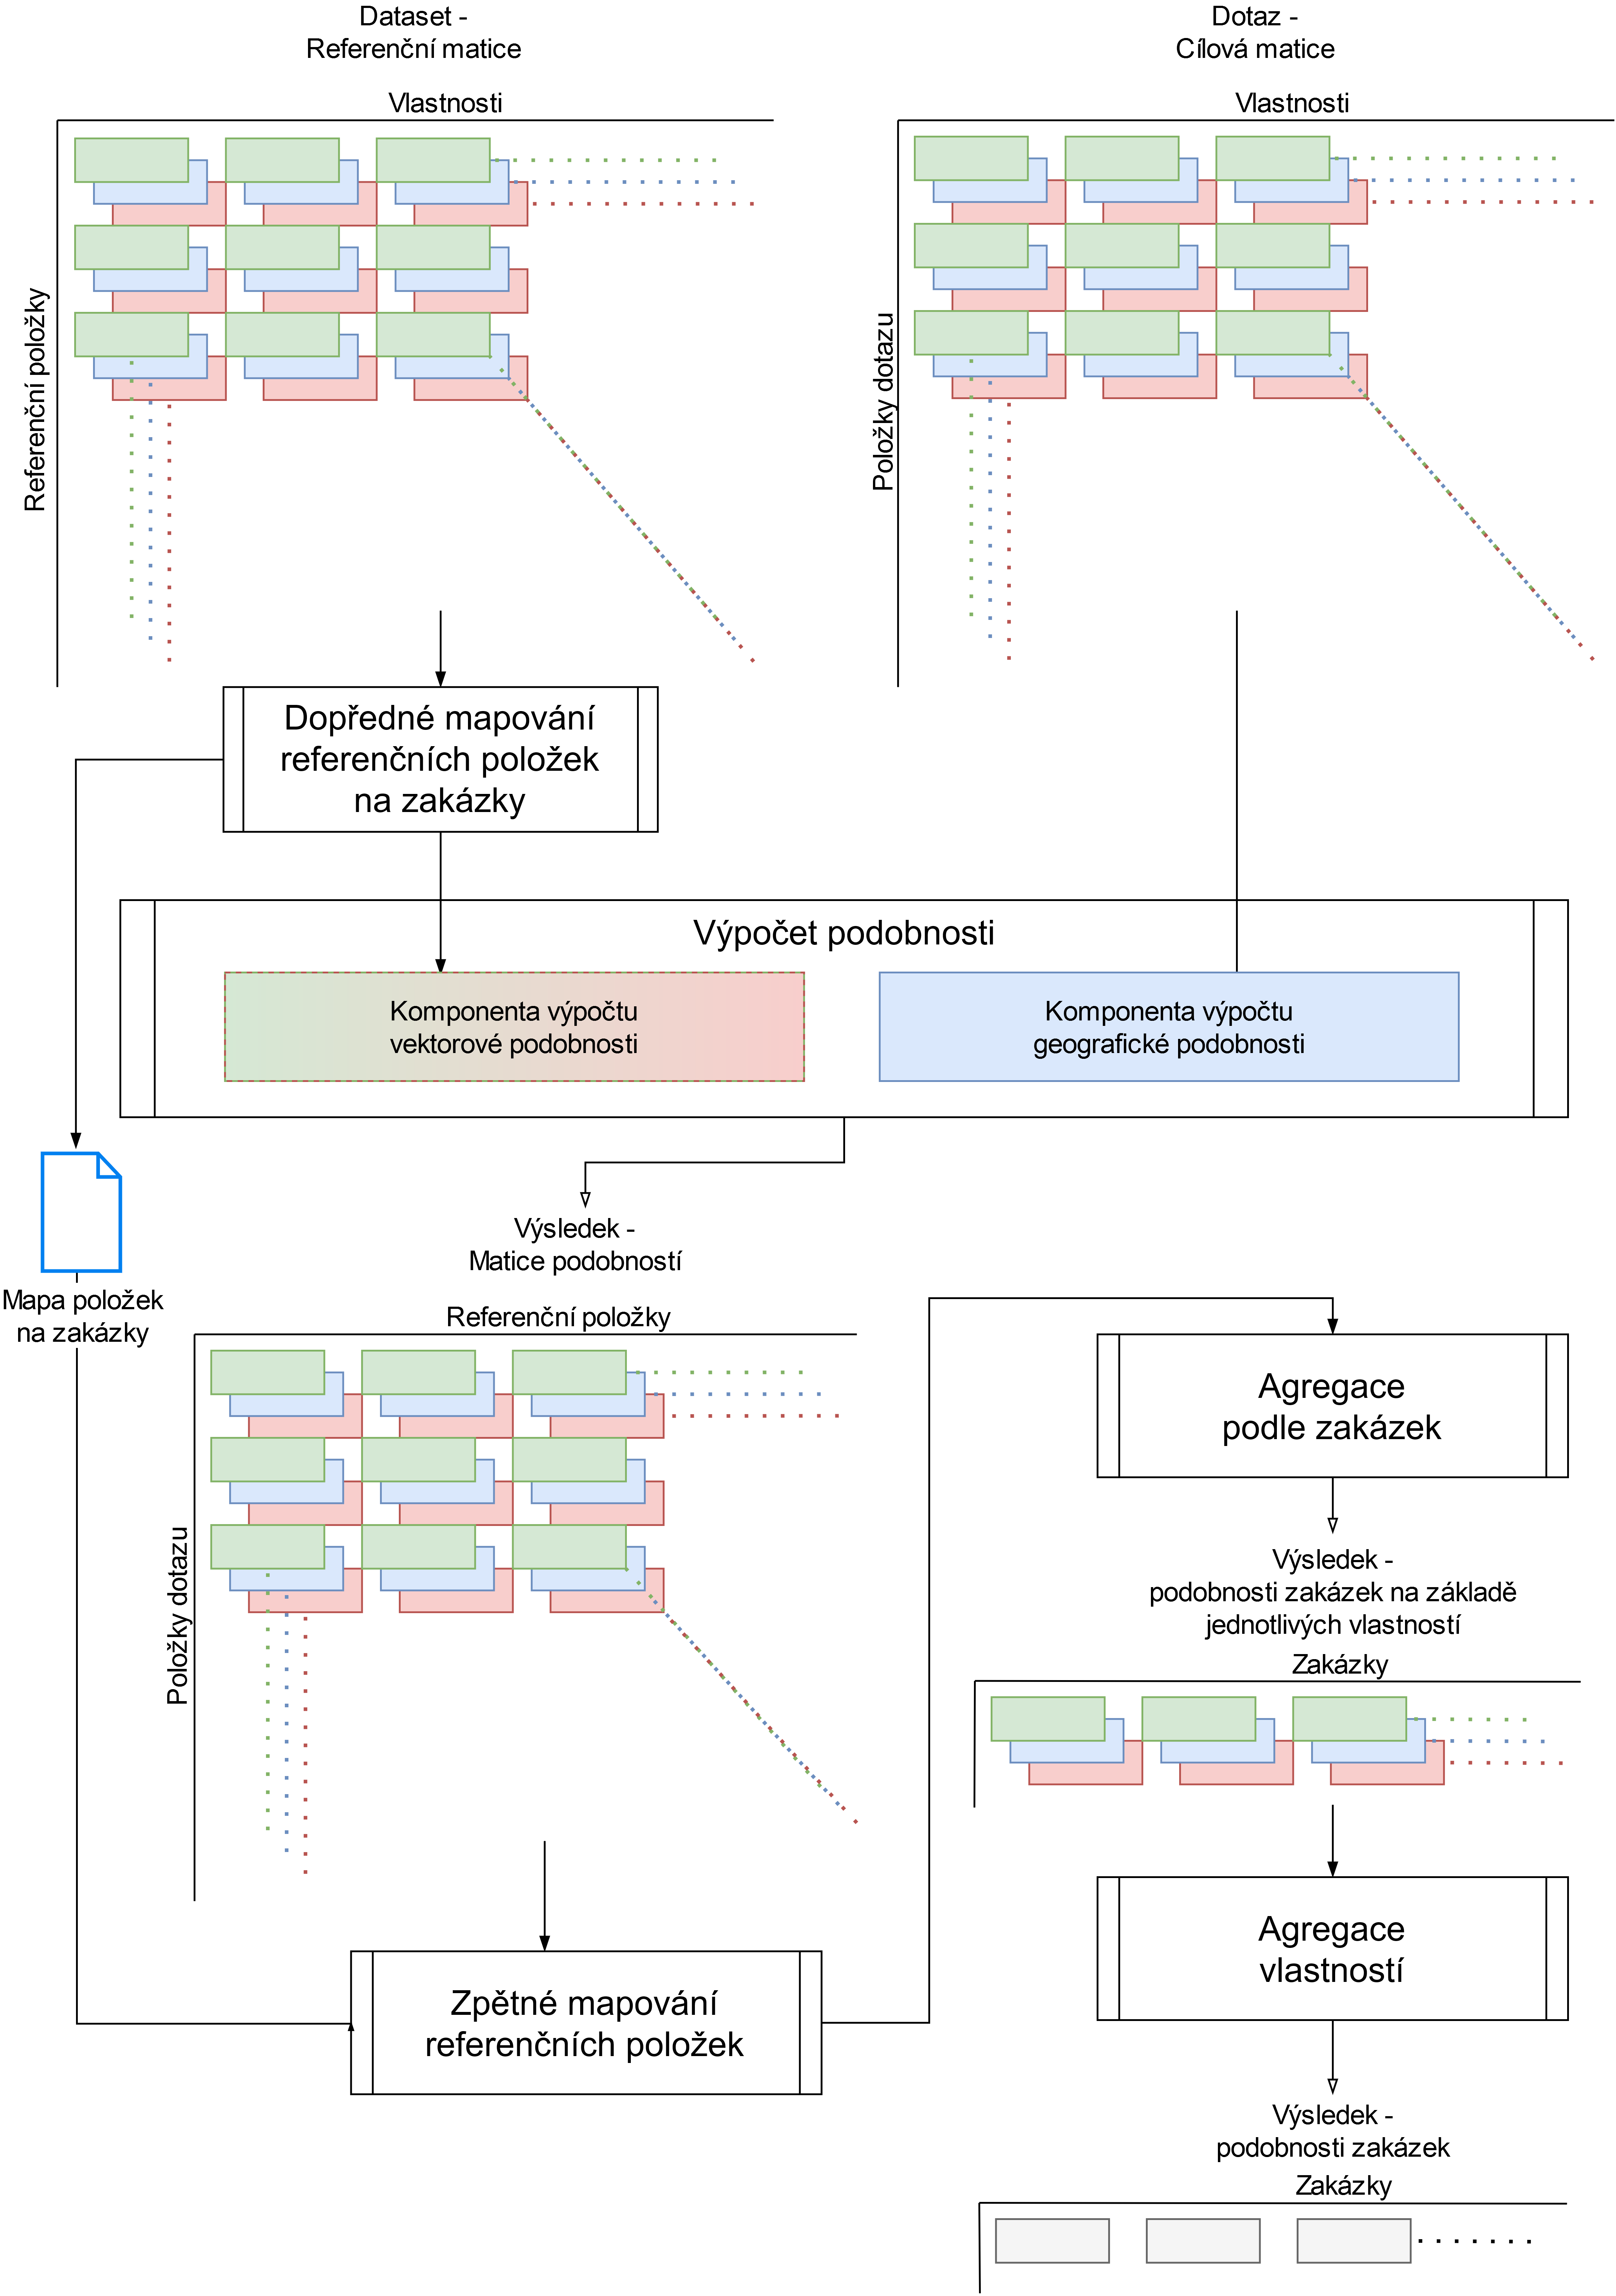
\includegraphics[width=\textwidth]{images/recommender_algorithm.png}
	\caption{Schéma výpočtu podobnosti}\label{fig:recommender_algorithm}
\end{figure}

Implementace této komponenty je adaptována pro zpracování dotazů více uživatelů najednou. V takovém případě jsou výsledky nejdříve agregovány podle samotných uživatelských dotazů.

\subsection{Lokalita zakázky}
\label{sec:feature_locality}

Lokalita zakázky je doplňková vlastnost rozšiřující možnosti dotazování. Vlastnost spočívá v identifikaci adresy sídla zadavatele zakázky, jak zmiňuji v kapitole \ref{sec:locality&subsub_extraction}. Tato vlastnost je na schématech \ref{fig:recommenderfeatures} a \ref{fig:recommender_algorithm} reprezentovaná modře.

Adresu sídla každého zadavatele převádím na GPS souřadnice komponentou \ref{sec:locality&subsub_extraction}.

Z důvodu, že se výpočet geodetické vzdálenosti ukazuje být příliš náročný (viz. tabulka \ref{table:experiment_similarity3}) pro počítání mezi početnějším množství bodů a přesná vzdálenost není pro účely komponenty nezbytná, implementuji aproximační algoritmus výpočtu vzdálenosti v euklidovském prostoru. 

Aproximace spočívá v převedení GPS souřadnic na souřadnice 2D prostoru vynásobením patřičné souřadnice vzdáleností odpovídající jednomu stupni na území České republiky, které jsou 111.32 kilometru na jeden stupeň zeměpisné šířky (všude na Zemi) a 71.94 kilometru na jeden stupeň zeměpisné délky na úrovni ČR (experimentálně zjištěno optimalizací oproti geodetické vzdálenosti na množině 100 cílových a 1000 referenčních bodů náhodně vygenerovaných v okolí geografického těžiště ČR). Optimalizovaným parametrem dosahuji na dané množině bodů odchylky 0.68 \%  za řádově tisícinásobného zrychlení (viz. výsledky tabulky \ref{table:experiment_similarity3}).

Odvozené 2D souřadnice dále využívám komponentou výpočtu euklidovské podobnosti (viz. kapitola \ref{sec:component_euclidean_similarity}).

\begin{table}[h!]
\centering
\begin{tabular}{ |l|l|r| }
\hline
Knihovna & Funkce & Čas [s] \\\hline
\hline
\textit{geopy} & \textit{geodesic} & 25.0000 \\
\textit{geopy} & \textit{great\_circle} & 1.9500 \\
--- & vlastní & 0.0035 \\\hline
\end{tabular}
\caption{Měření doby výpočtu algoritmů pro výpočet geografické vzdálenosti}
\label{table:experiment_similarity3}
\end{table}


Na lokalitu jednotlivých zakázek v podobě referenčních bodů sestavuji dotaz ve stejné reprezentaci cílových bodů složený z:
\begin{enumerate}
    \item adresy či GPS souřadnic přímého vyhledávání,
    \item lokality danou uživatelským profilem.
\end{enumerate}

Komponenta výpočtu geografické podobnosti vrací jako výsledek matici podobnosti cílového bodu vůči referenčnímu bodu každé zakázky.

Implementace této komponenty je adaptována pro zpracování dotazů více uživatelů najednou. V takovém případě jsou výsledky nejdříve agregovány podle samotných uživatelských dotazů.


\subsection{Předmět podnikání zadavatele}
\label{sec:feature_entity_subject}

Předmět podnikání zadavatele zakázky je doplňková vlastnost dále rozšiřující možnosti dotazování. Vlastnost spočívá v identifikaci předmětu podnikání zadavatele zakázky, jak zmiňuji v kapitole \ref{sec:locality&subsub_extraction}. Na schématech \ref{fig:recommenderfeatures} a \ref{fig:recommender_algorithm} je tato vlastnost reprezentovaná červeně.

Dále pracuji s touto vlastností totožně jako s předmětem zakázky, tedy -- embedding -- výpočet vektorové podobnosti -- agregace (viz. kapitola \ref{sec:feature_subject}).


\subsection{Kombinace vlastností}

Jak zmiňuji v úvodu kapitoly \ref{sec:recommender_design}, vlastnosti lze kombinovat pro složení komplexního dotazu.

Skládání dotazu a datasetu v tom případě probíhá najednou složením daných vlastností do jedné kolekce, přičemž komponenty výpočtu podobnosti jednotlivých vlastností využívají jim odpovídající vlastnost nezávisle na ostatních. Výpočet podobnosti a agregace probíhají totožně pro každou ze složených vlastností.

Navíc je zde akorát poslední krok -- agregace vlastností. Tento krok se provádí na úrovni jednotlivých zakázek tak, že se z výsledků podobnosti jednotlivých vlastností počítá vážený průměr.

Pro zajištění určité míry explorace doporučování implementuji komponentě možnost aplikace náhodného šumu na výslednou podobnost.

\subsection{Vyhodnocení}

V kapitole \ref{sec:recommender_evaluation} pojednávám o možnostech vyhodnocování doporučovacích systémů. V rámci této práce ovšem nejsem schopný zmiňovanými způsoby navržený systém vyhodnocovat hned ze dvou důvodů.

Zaprvé nemám k dispozici dataset záznamů uživatelských interakcí, na základě kterého by mohl být systém laděn a automaticky vyhodnocován.

Zadruhé systém není v době řešení této práce v produkčním provozu, kdy by bylo možné za běhu zaznamenávat uživatelské chování a na základě toho dále systém vyhodnocovat.

Funkčnost navrženého systému je ovšem převážně algoritmická a neobsahuje části vykazující skryté chování, které by bylo nutné automaticky ladit či vyhodnocovat pro jeho základní funkčnost.


\chapter{Aplikace}

Doporučovací systémy se tradičně uplatňují v prostředích s vysokým počtem přistupujících uživatelů. Příkladem jsou populární online platformy jako je Youtube, Netflix, Facebook, Spotify a jiné. Pro demonstraci systému realizovaného v mé práci tak vytvářím webovou aplikaci, která poskytuje uživatelské rozhraní k jeho použití. V této kapitole stručně shrnuji vlastnosti a možnosti tohoto rozhraní, které podchycují funkčnost celého systému. Pro ukázku dále uvádím konkrétní případ užití s ilustrovaným popisem funkčnosti.
\newpage

\section{Funkce}

Aplikace umožňuje uživateli využít systém ve dvou různých módech:
\begin{enumerate}
    \item anonymní mód -- omezený mód, který lze použít bez nutnosti přihlášení,
    \item privilegovaný mód -- rozšířený mód, do kterého lze vstoupit pomocí přihlášení.
\end{enumerate}

Aplikace dále disponuje dvěma základními funkcemi:
\begin{enumerate}
    \item vyhledávání zakázek -- vyhledávání konkrétních zakázek na základně parametrů zadaných uživatelem; je nezávislé na konkrétním uživateli,
    \item doporučování zakázek -- automatické nabízení vybraných zakázek bez nutnosti exaktního uživatelského vstupu; řídí se profilem uživatele.
\end{enumerate}

Tyto dvě funkce se principiálně odlišují pouze stylem získání vstupu, na základě kterého systém dohledává relevantní zakázky. V obou případech je výsledkem množina několika zakázek, které aplikace ve stručné reprezentaci zobrazuje na stránce v podobě seznamu s možností prostupu do detailu jednotlivých zakázek. V detailu jsou poté kompletně zobrazeny všechny informace dané zakázky s odkazem na profil\footnote{profil zadavatele -- nezaměňovat s uživatelským profilem; více viz. kapitola \ref{data&domain_dokumenty_vz}} zadavatele, kde je zveřejněná.

Vyhledávání je možné provádět bez nutnosti přihlášení, tedy i v anonymním módu, zatímco funkce doporučování je zpřístupněna pouze v privilegovaném módu, kde se řídí uživatelským profilem. Uživatelské přihlašování aplikace simuluje na základě unikátního identifikátoru nebo čísla IČO, podle kterého inicializuje uživatelský profil.

V privilegovaném módu jsou uživateli na hlavní stránce aplikace nabízeny zakázky ve čtyřech sekcích:
\begin{enumerate}
    \item Zakázky z blízkého okolí (\uv{Blízké zakázky}) -- podle lokality uvedené na profilu a lokality zadavatelů zakázek (kap. \ref{sec:feature_locality}),
    \item Zakázky s předmětem zájmu (\uv{Zakázky se zajímavým předmětem}) -- podle položek zájmu uvedených na profilu a předmětu jednotlivých zakázek (kap. \ref{sec:feature_subject}),
    \item Zakázky podobných zadavatelů (\uv{Zakázky podobných zadavatelů}) -- též podle položek zájmu, ale oproti předmětu podnikání zadavatelů zakázek (kap. \ref{sec:feature_entity_subject}),
    \item všechna tři kritéria dohromady (\uv{Zakázky pro Vás}).
\end{enumerate}

Aplikace umožňuje uživateli informace svého profilu upravovat a měnit tak svou lokalitu a předmět zájmu.

Podle vyhledávání a prostupů na detaily jednotlivých zakázek aplikace aktualizuje profil daného uživatele tak, aby se doporučování přizpůsobovalo jeho chování. To řeším přidáváním položek předmětů vyhledávání a daných zakázek do uživatelského profilu jako doplňkové položky zájmu. Tyto položky jsou také vidět na profilu uživatele.

\subsection{Technologie}

Vzhledem k převážnému používání jazyku Python v ostatních částech práce tento jazyk používám i pro vytvoření webové aplikace, přičemž aplikaci stavím konkrétně pro její flexibilitu a jednoduchost na technologii \textit{Flask}\footnote{Flask -- Python webový framework;\newline
dokumentace dostupná z https://flask.palletsprojects.com/en/1.1.x/}.

V rámci celé práce používám databázi \textit{Postgres} pro průběžné ukládání zpracovávaných dat, ke které vytvářím přístupovou komponentu za použití knihovny \textit{psycopg2}\footnote{psycopg2 -- Python adaptér pro Postgres databázi;\newline
dostupný z https://pypi.org/project/psycopg2/}. Pro napojení aplikace na databázi tak plně využívám této komponenty.

Inicializace aplikace je závislá na konfiguraci předané speciálním souborem, ve kterém jsou specifikované parametry:
\begin{itemize}
    \item úroveň a název souboru pro logování,
    \item nastavení pro inicializaci uživatelské \uv{session},
    \item přístupové údaje k databázi,
    \item cesta k modelu pro embedder (viz. kapitola \ref{sec:component_embedding}).
\end{itemize}
\newpage

\section{Ukázka použití aplikace}
Při prvním načtení se uživatel ocitne v anonymním módu aplikace. V tomto módu je mu umožněno plnohodnotné vyhledávání bez vlivu algoritmu doporučování. Na rozdíl od privilegovaného módu se tak uživateli nezobrazují postranní sekce přizpůsobované podle uživatelského profilu, jak je zachyceno na obrázku \ref{fig:pcrec_anonymous_vs_priviledged}.
\begin{figure}[!h]
\centering
\begin{subfigure}{.5\textwidth}
  \centering
	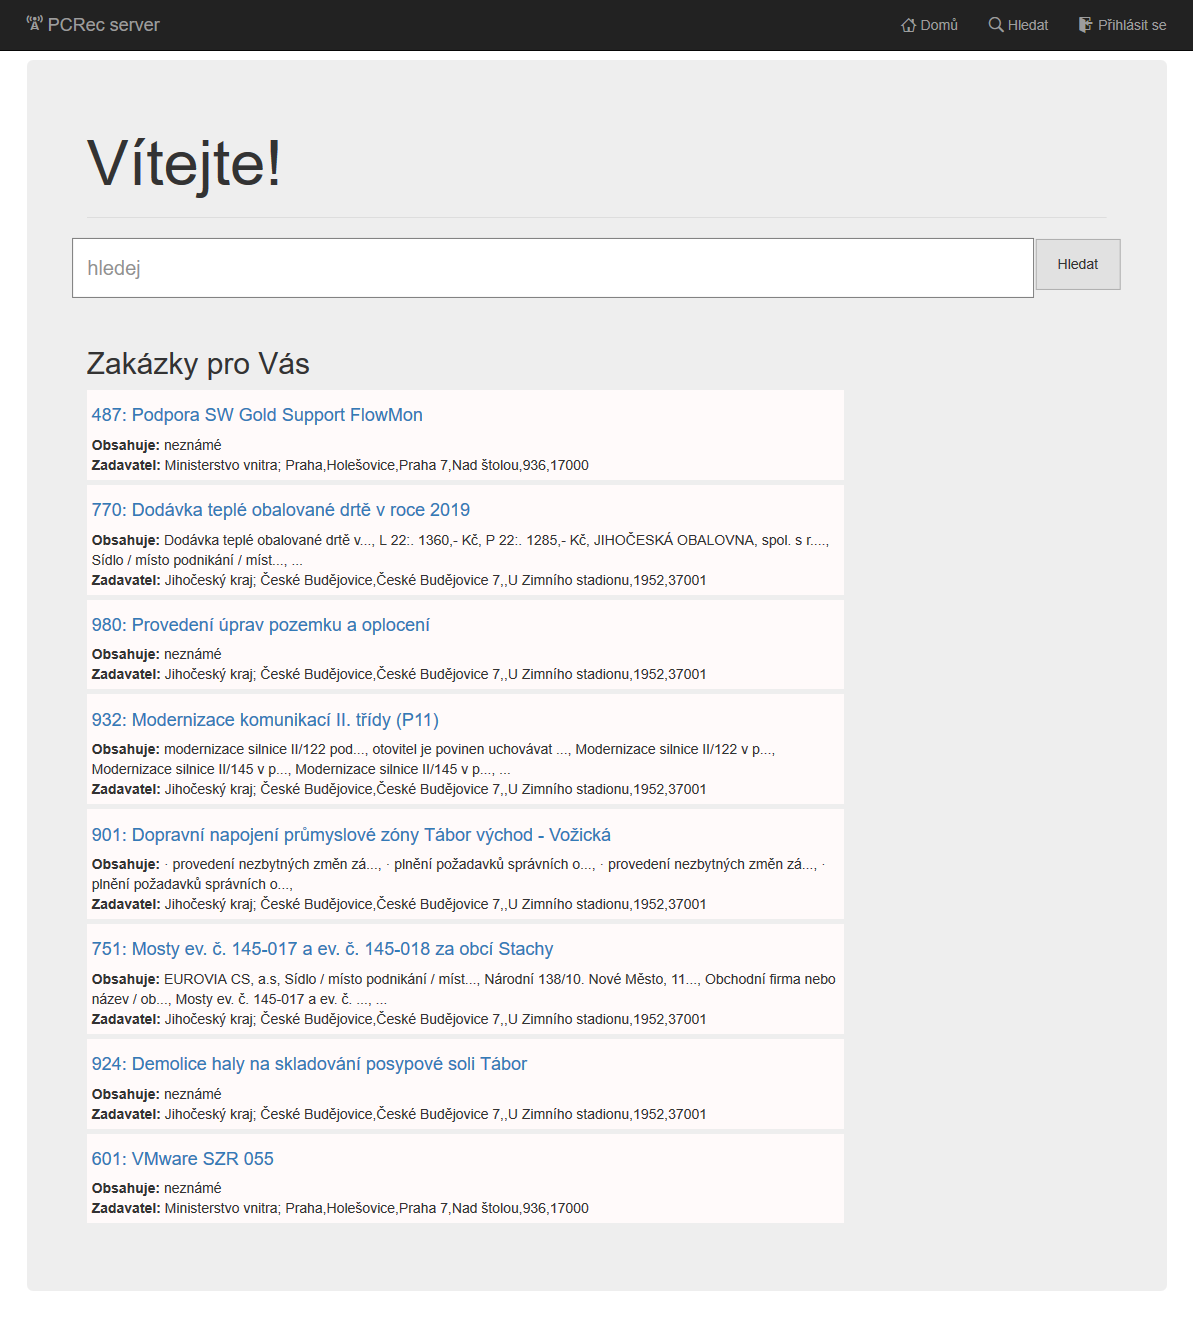
\includegraphics[width=\textwidth]{images/pcrec/pcrec_anonymous.png}
	\caption{Anonymní mód aplikace}\label{fig:pcrec_anonymous}
\end{subfigure}%
\begin{subfigure}{.5\textwidth}
  \centering
	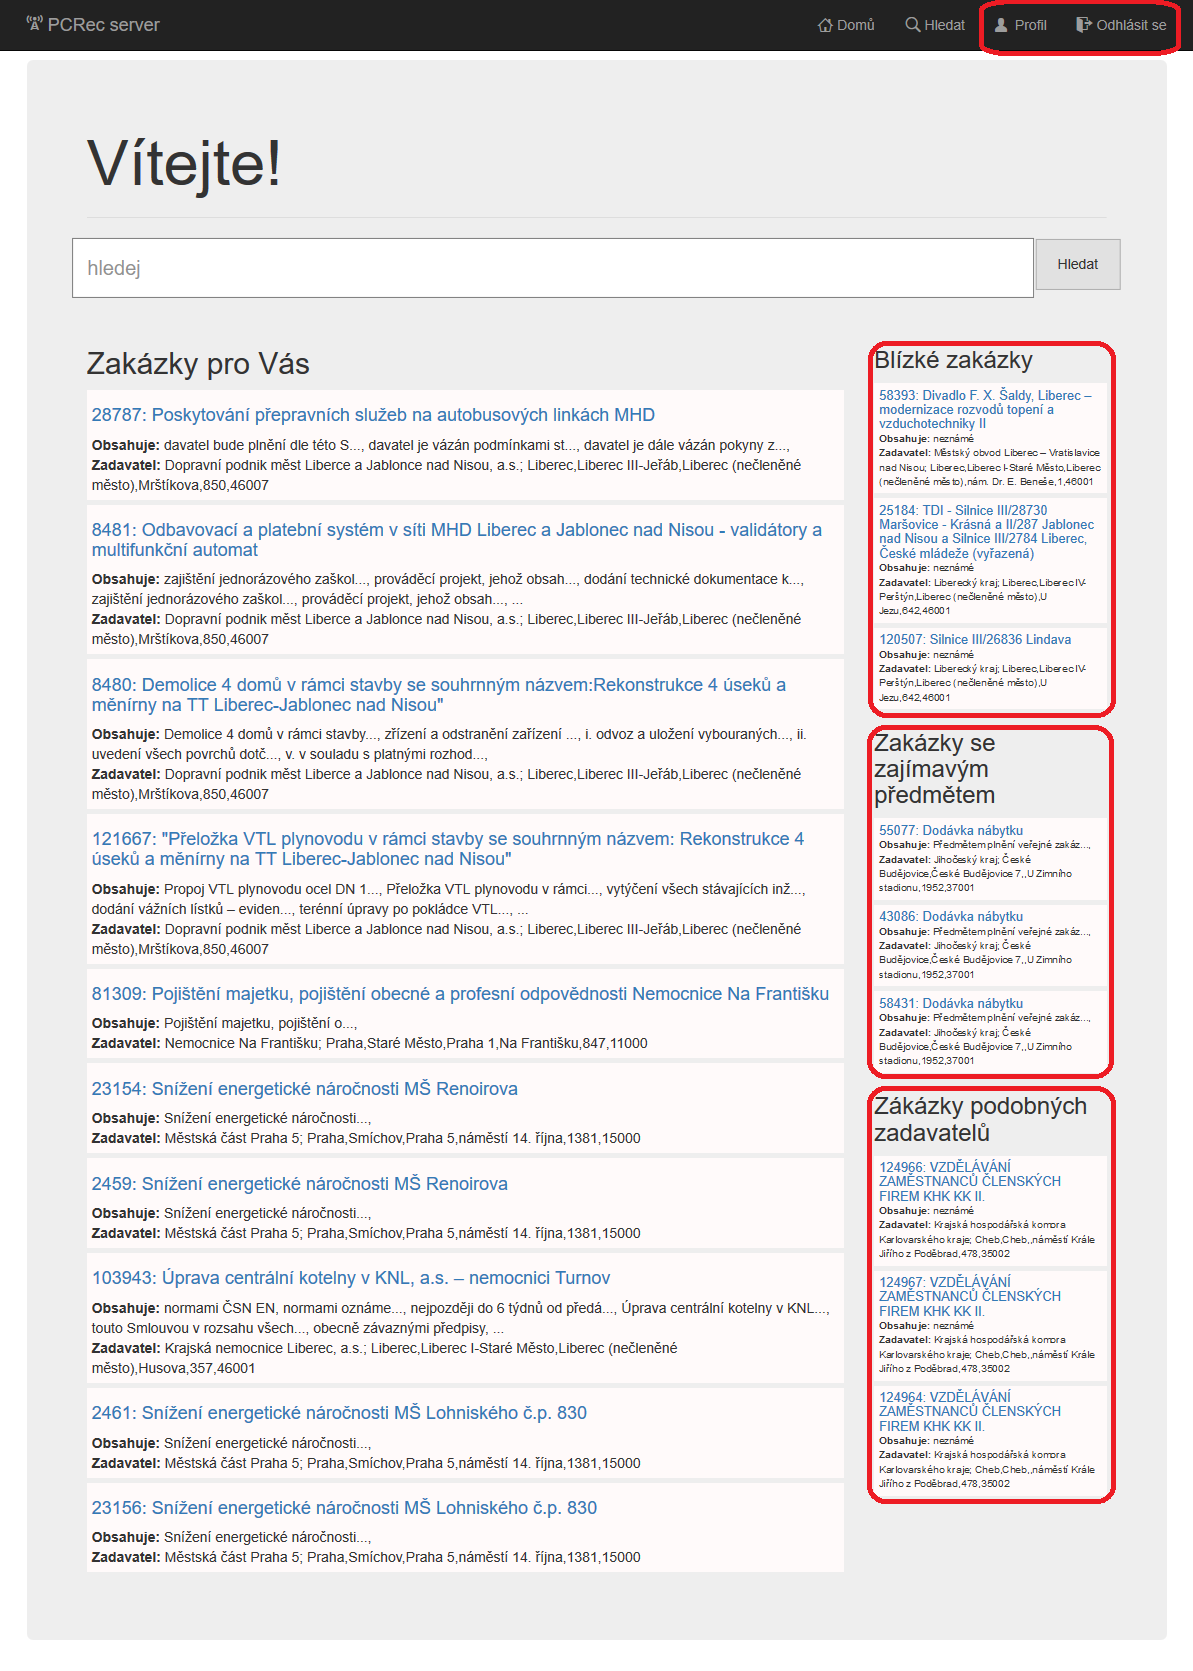
\includegraphics[width=\textwidth]{images/pcrec/pcrec_main_edit.png}
	\caption{Privilegovaný mód aplikace}\label{fig:pcrec_main_edit}
\end{subfigure}
\caption{Porovnání anonymního a privilegovaného módu aplikace}
\label{fig:pcrec_anonymous_vs_priviledged}
\end{figure}
\newpage

Uživatel může vstoupit do privilegovaného módu aplikace pomocí přihlášení s uživatelským identifikátorem, nebo číslem IČO.
% (viz. obrázek \ref{fig:pcrec_login})
Pokud zvolí přihlášení pomocí čísla IČO, je mu automaticky inicializován profil s položkami předmětu podnikání osoby s daným číslem IČO, jako je vidět na obrázku
\ref{fig:pcrec_profile1_edit}.
% \begin{figure}\centering
% 	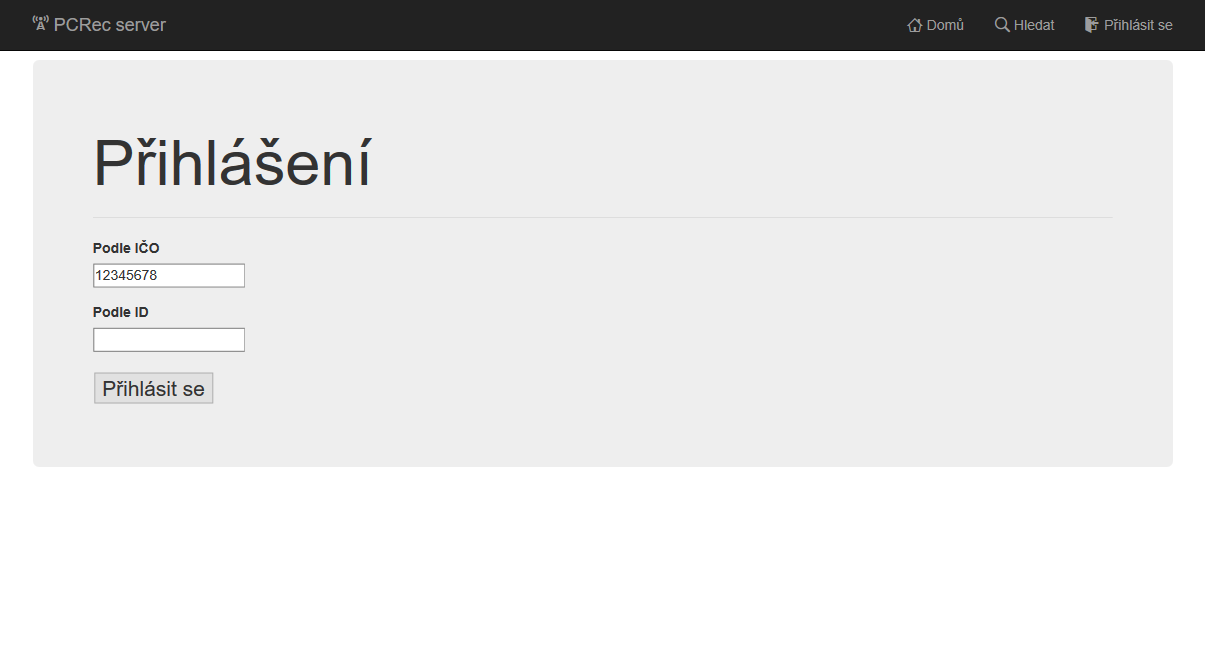
\includegraphics[width=\textwidth]{images/pcrec/pcrec_login.png}
% 	\caption{Přihlášení do aplikace}\label{fig:pcrec_login}
% \end{figure}

Jakmile je uživatel v privilegovaném módu, aplikace mu začne nabízet doporučované zakázky na základě jeho profilu. V tomto módu aplikace zaznamenává uživatelovo chování do jeho profilu. Pokud tedy uživatel zadá například vyhledávání \uv{stavba bazénu} a prostoupí do detailu některé z vyhledaných zakázek, jako je znázorněno na obrázku \ref{fig:pcrec_search_result_edit}, jeho profil se zaktualizuje podle předmětu vyhledávání a dané zakázky (viz. obrázek \ref{fig:pcrec_profile1_edit}).
% \begin{figure}\centering
% 	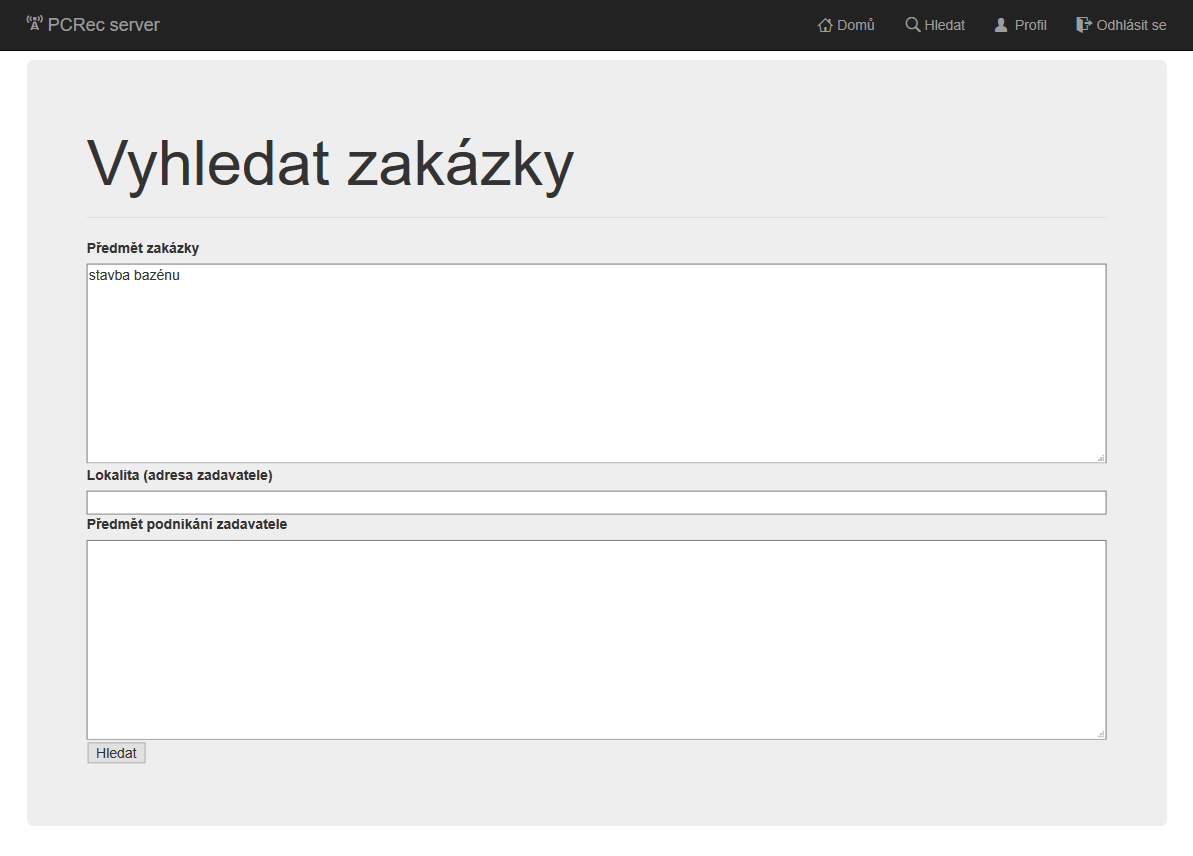
\includegraphics[width=\textwidth]{images/pcrec/pcrec_search.png}
% 	\caption{Vyhledávání podle parametrů}\label{fig:pcrec_search}
% \end{figure}
\begin{figure}\centering
	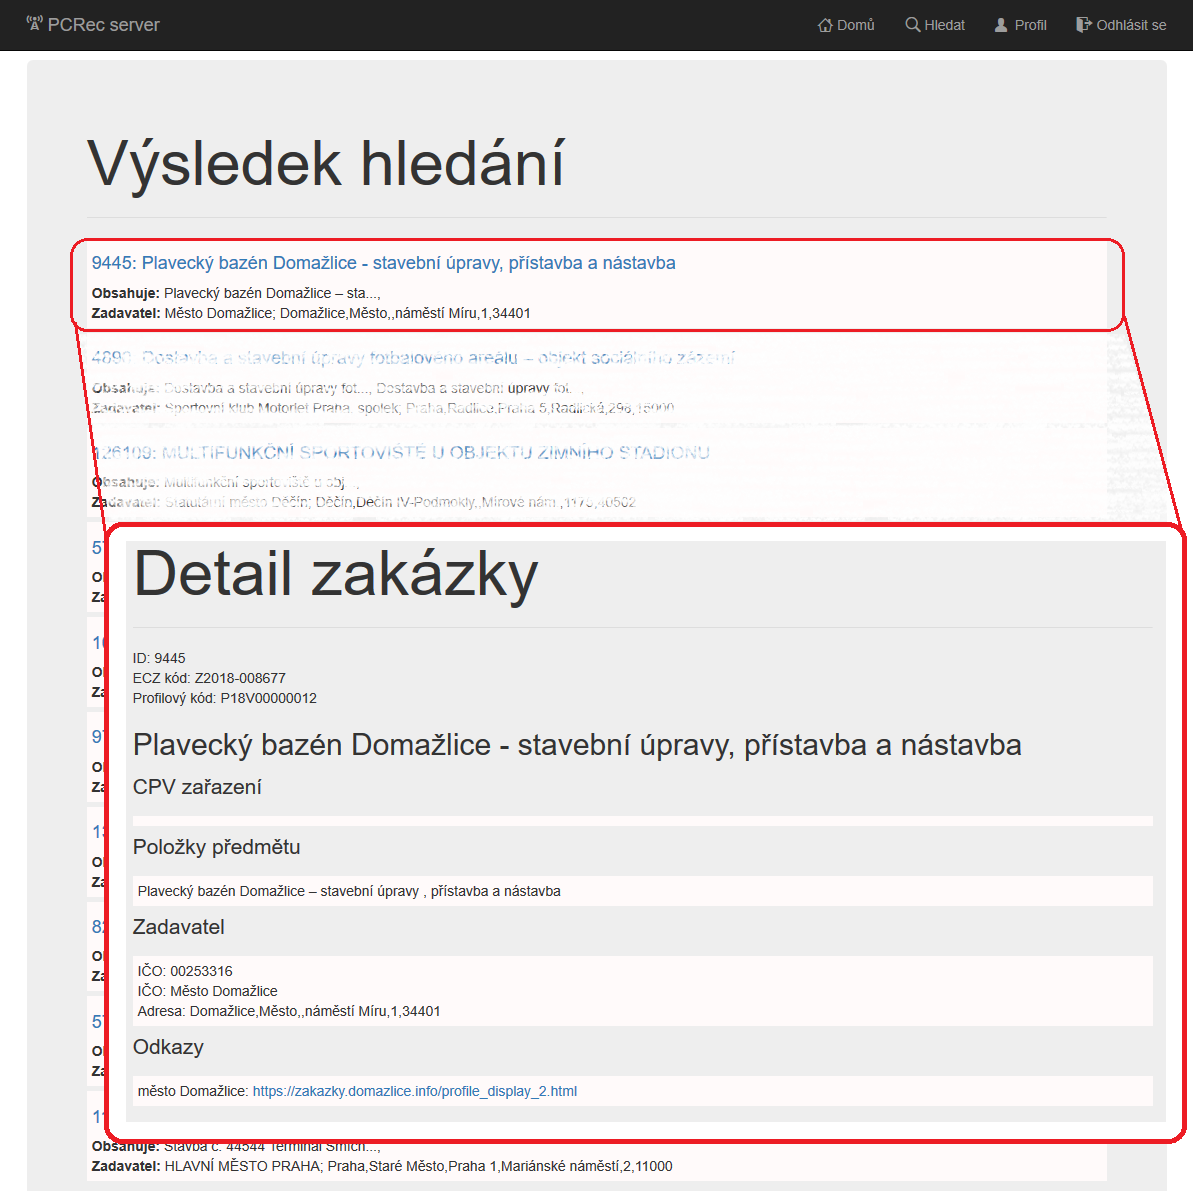
\includegraphics[width=\textwidth]{images/pcrec/pcrec_search_result_edit3.png}
	\caption{Výsledek vyhledávání podle předmětu \uv{stavba bazénu} s prostupem na detail zakázky}\label{fig:pcrec_search_result_edit}
\end{figure}
\begin{figure}\centering
	\includegraphics[width=\textwidth]{images/pcrec/pcrec_profile_edit.png}
	\caption{Porovnání čistě inicializovaného a aktualizovaného profilu}\label{fig:pcrec_profile1_edit}
\end{figure}
% \begin{figure}\centering
% 	\includegraphics[width=\textwidth]{images/pcrec/pcrec_profile2.png}
% 	\caption{Aktualizovaný profil}\label{fig:pcrec_profile2}
% \end{figure}

Aktualizace profilu má dále za důsledek přizpůsobení obsahu domovské stránky uživatele, jak je znázorněno na obrázku \ref{fig:pcrec_recommended}.
\begin{figure}\centering
	\includegraphics[width=\textwidth]{images/pcrec/pcrec_recommended_edit2.png}
	\caption{Ukázka doporučování aplikace přizpůsobeného předmětu zájmu \uv{stavba bazénu}}\label{fig:pcrec_recommended}
\end{figure}

\chapter{Budoucí rozšíření systému}

V práci se mi podařilo zprovoznit prototyp doporučovacího systému, který do určité míry funguje. Pro nasazení v reálném prostředí by však bylo vhodné či~přímo nutné systém rozšířit o další funkčnosti. O těchto rozšířeních diskutuji v této kapitole v pořadí od rozšíření s nejvyšší prioritou po rozšíření méně důležitá.

\newpage
\section{Funkční celky k rozšíření}
\subsection{Aktualizace dat}

V práci jsem používal různé datasety, které byly více či méně aktuální. Ani zdaleka jsem však neobsáhl celou množinu dat českých veřejných zakázek. 

Produkční provoz systému by byl závislý na kompletním datasetu, který se na denní bázi průběžně rozšiřuje. Meziročně v česku přibývá zhruba 50~tisíc zakázek, což vychází na více jak 100 zakázek denně. Za předpokladu průměru 10 dokumentů na zakázku to poté vychází zhruba na půl milionu dokumentů za rok.

V rámci práce jsem vytvořil databázi dokumentů zakázek za období leden až červen 2019. Celkem 900 tisíc dokumentů ke 130 tisícům zakázek, kde se ovšem dle mého zjištění vyskytuje značné množství duplicit. Tato databáze s dokumenty ve formátu prostého textu přesahuje velikosti 4 GB. Lze tedy předpokládat, že s přírůstkem 50 tisíc zakázek za rok bude velikost databáze úměrně růst rychlostí alespoň nízkých jednotek GB za rok.

Data je ovšem potřeba udržovat co nejaktuálnější, což by pravděpodobně šlo řešit každodenními aktualizacemi databáze zakázek, které by mohly být prováděny například v pravidelných nočních \uv{jobech}.

\subsection{Aplikace}

Z pohledu uživatele je aplikace nejdůležitější částí celého systému. V práci jsem vytvořil jednoduchou webovou aplikaci pro demonstrační účely systému, avšak pro reálné použití je nedostačující.

Pro dosažení maximální uživatelské spokojenosti by bylo potřeba vytvořit webovou aplikaci za použití vhodných moderních webových a bezpečnostních technologií. Jedním ze slabých míst současného řešení je též komponenta pro komunikaci s databází, která se jeví jako tzv. úzké hrdlo v odezvě systému.

Uživatelský profil současně aplikace pouze simuluje, což by bylo potřeba nahradit kompletním robustním řešením.

\subsection{Pokročilejší algoritmy výpočtu podobnosti}

Přestože je úzkým hrdlem současné implementace aplikace databázová vrstva, je možné, že by se výkonnostní problémy dotazování na databázi podařilo vyřešit a nejpomalejší částí systému by se tak stal samotný výpočet podobnosti.

V práci jsem řešil optimalizaci výpočtu podobnosti za použití funkcí pro maticové operace knihovny \textit{numpy}, která se zaměřuje na efektivitu výpočtů.
Touto implementací trvá výpočet podobnosti obyčejného dotazu oproti zhruba milionu položkám řádově jednotky sekund, přičemž takové množství dat odpovídá zhruba ročnímu přírůstku (50 tisíc zakázek s průměrným počtem 20 položek na zakázku).

Pokud by byla efektivita současné implementace v produkci nedostačující, bylo by možné pro snížení velikosti počítaných matic algoritmus výpočtu podobnosti rozšířit o shlukování (\uv{clusterování}) či agregaci položek. V případě clusterování by se podobnost počítala nejdříve na úrovni jednotlivých clusterů a poté k~jednotlivým položkám. Agregace položek by mohla probíhat za cenu ztráty určité informace jak na úrovni uživatelského profilu, tak na úrovni zakázek.

\subsection{Diverzifikace a explorace doporučování}

Současný algoritmus doporučování umožňuje aplikaci náhodného šumu na výpočet podobnosti, čímž lze do určité míry nastavovat poměr explorace a exploatace doporučování. Stále ale může docházet k výskytům příliš podobných výsledků (slabá diverzifikace).

Bylo by tedy vhodné aplikovat některé pokročilejší metody pro balancování poměru explorace a exploatace a dosažení objektivní diverzifikace výsledků.
Jako jedna z možností jak toho dosáhnout se nabízí clusterování podobných položek za účelem vybírání pouze podmnožiny výsledků z~daného clusteru.

\subsection{Možnosti filtrování zakázek}

Možnosti filtrování navrženého doporučovacího systému jsou omezené pouze na vlastnosti předmětu zakázky, lokality a předmětu podnikání zadavatele. Pro reálné užití systému by bylo vhodné po vzoru jiných současných systémů doplnit možnosti filtrování podle dalších vlastností zakázek jako je jejich kategorické či časové zařazení, stav, cenový rozsah a podobně.

\subsection{Klasifikátor CPV}

Na základě analýzy datasetu v kapitole \ref{sec:cpv_distribution} uzavírám CPV klasifikaci dokumentů s odůvodněním nedostatečného datasetu.

V případě, že by se dostatečný dataset podařilo vytvořit, bylo by možné učit klasifikátor pro automatické rozpoznávání kategorie dokumentů a tudíž i zakázek.

\subsection{Katalog produktů}

V kapitole \ref{sec:product_catalog} pojednávám o možnostech využití katalogu produktů.

Takový katalog se mi nepodařilo v rámci práce opatřit, ovšem v případě, že by se to podařilo, dalo by se s jeho pomocí získat další hodnotné informace o předmětu zakázek.

\subsection{Vlastní model pro embedding dokumentů}

V rámci zjednodušení kapitoly embeddingu dokumentů (\ref{sec:document_embedding}) jsem v práci použil předučené jazykové modely. Funkčnost modelů je ovšem závislá na povaze korpusu, na kterém jsou učené a proto by bylo vhodné v doméně veřejných zakázek naučit nebo alespoň vyladit model na korpusu, který by byl vytvořený z dokumentací samotných veřejných zakázek.

\subsection{Ladění extrakce předmětu}
Extrakce předmětu z textu je v oboru zpracování přirozeného jazyka problém sám o sobě, kterým se dlouhodobě zabývá mnoho odborníků.

Algoritmy extrakce předmětu navržené a implementované v této práci plní do jisté míry svůj účel, ovšem stále za přítomnosti nezanedbatelného množství falešných pozitivních i negativních nálezů. V tom smyslu by tedy mohla extrakce předmětu zakázek jít dále řešit jako celý samostatný projekt.


\begin{conclusion}
	V úvodu práce provádím rešerši současných systémů podporujících elektronické řízení a vyhledávání českých veřejných zakázek. Pojednávám o jejich vlastnostech a mezerách, na které se tato práce zaměřuje.
	
	V rámci práce jsem navrhl a implementoval content-based doporučovací systém pro české veřejné zakázky. Doporučování je založeno na základě vybraných vlastností zakázek a uživatelském preferenčním profilu obsahujícím podobné vlastnosti.
	
	Doporučování se uživateli přizpůsobuje podle jeho chování v aplikaci ve smyslu aktualizace jeho profilu informacemi zakázek, které si prohlédl.
	
	Pro získávání vlastností jsem navrhl a implementoval proces extrakce informací z dokumentace veřejných zakázek a systémů poskytujících nejen data VZ.
	
	Jako hlavní vlastnost zakázek jsem použil jejich předmět plnění, pro který jsem navrhl a implementoval algoritmy extrakce z textu dokumentace. Pro podchycení sémantické informace předmětu používám embedding textu. Volbu modelu pro embedding opírám o experimentální vyhodnocení současných state-of-the-art metod.
	
	Projekt je implementovaný s modulární architekturou, kde jednotlivé komponenty jsem zdokumentoval pro možnost sestavení funkčního prototypu aplikace doporučovacího systému. Pro demonstraci jsem vytvořil jednoduchou webovou aplikaci, která umožňuje uživateli využít důležité vlastnosti systému.
	
	V závěru práce pojednávám o možnostech rozšíření systému nutných pro jeho nasazení v reálném prostředí.
	
	Celý projekt je vybudovaný za pomocí open-source technologií a pod open-source licencí je též vydaný a dostupný v repozitáři laboratoře otevřených dat  \textit{opendatalabcz/public-contract-recommendation}\footnote{opendatalabcz/public-contract-recommendation repozitář\newline
	-- dostupný z https://github.com/opendatalabcz/public-contract-recommendation}.
\end{conclusion}

\bibliographystyle{csn690}
\bibliography{mybibliographyfile}

\appendix

% \chapter{Ukázka použití aplikace}
% \label{sec:application_use_case}



\chapter{Seznam použitých zkratek}
% \printglossaries
\begin{description}
    \item[API] Application Programming Interface
    \item[ARES] Administrativní registr ekonomických subjektů
    \item[BERT] Bidirectional Encoder Representations from Transformers
    \item[BOW] Bag-of-words
    \item[CBOW] Continuous Bag-of-words
    \item[CPV] Common Procurement Vocabulary
    \item[ČR] Česká republika
    \item[ECZ] Evidenční číslo zakázky
    \item[ELMo] Embeddings from Language Model
    \item[GB] Gigabyte
    \item[GPS] Global Positioning System
    \item[GPT] Generative Pre-Training Transformer
    \item[HDP] Hrubý domácí produkt
    \item[IČO] Identifikační číslo osoby
    \item[ISVZ] Informační systém o veřejných zakázkách
    \item[LDA] Latent Dirichlet Allocation
    \item[LSTM] Long Short-term Memory
    \item[NLP] Natural Language Processing
    \item[PDT] Prague Dependency Treebank
    \item[PLSI] Probabilistic Latent Semantic Indexing
    \item[POS] Part-of-speech
    \item[STS] Semantic Textual Similarity
    \item[tf-idf] term frequency – inverse document frequency
    \item[UD] Universal Dependencies
    \item[ULMFiT] Universal Language Model Fine-tuning
    \item[USE] Universal Sentence Encoder
    \item[VZ] Veřejná zakázka
    \item[WMD] Word Mover's Distance
    \item[WME] Word Mover's Embedding
\end{description}


% % % % % % % % % % % % % % % % % % % % % % % % % % % % 
% % Tuto kapitolu z výsledné práce ODSTRAŇTE.
% % % % % % % % % % % % % % % % % % % % % % % % % % % % 
% 
% \chapter{Návod k~použití této šablony}
% 
% Tento dokument slouží jako základ pro napsání závěrečné práce na Fakultě informačních technologií ČVUT v~Praze.
% 
% \section{Výběr základu}
% 
% Vyberte si šablonu podle druhu práce (bakalářská, diplomová), jazyka (čeština, angličtina) a kódování (ASCII, \mbox{UTF-8}, \mbox{ISO-8859-2} neboli latin2 a nebo \mbox{Windows-1250}). 
% 
% V~české variantě naleznete šablony v~souborech pojmenovaných ve formátu práce\\_kódování.tex. Typ může být:
% \begin{description}
% 	\item[BP] bakalářská práce,
% 	\item[DP] diplomová (magisterská) práce.
% \end{description}
% Kódování, ve kterém chcete psát, může být:
% \begin{description}
% 	\item[UTF-8] kódování Unicode,
% 	\item[ISO-8859-2] latin2,
% 	\item[Windows-1250] znaková sada 1250 Windows.
% \end{description}
% V~případě nejistoty ohledně kódování doporučujeme následující postup:
% \begin{enumerate}
% 	\item Otevřete šablony pro kódování UTF-8 v~editoru prostého textu, který chcete pro psaní práce použít -- pokud můžete texty s~diakritikou normálně přečíst, použijte tuto šablonu.
% 	\item V~opačném případě postupujte dále podle toho, jaký operační systém používáte:
% 	\begin{itemize}
% 		\item v~případě Windows použijte šablonu pro kódování \mbox{Windows-1250},
% 		\item jinak zkuste použít šablonu pro kódování \mbox{ISO-8859-2}.
% 	\end{itemize}
% \end{enumerate}
% 
% 
% V~anglické variantě jsou šablony pojmenované podle typu práce, možnosti jsou:
% \begin{description}
% 	\item[bachelors] bakalářská práce,
% 	\item[masters] diplomová (magisterská) práce.
% \end{description}
% 
% \section{Použití šablony}
% 
% Šablona je určena pro zpracování systémem \LaTeXe{}. Text je možné psát v~textovém editoru jako prostý text, lze však také využít specializovaný editor pro \LaTeX{}, např. Kile.
% 
% Pro získání tisknutelného výstupu z~takto vytvořeného souboru použijte příkaz \verb|pdflatex|, kterému předáte cestu k~souboru jako parametr. Vhodný editor pro \LaTeX{} toto udělá za Vás. \verb|pdfcslatex| ani \verb|cslatex| \emph{nebudou} s~těmito šablonami fungovat.
% 
% Více informací o~použití systému \LaTeX{} najdete např. v~\cite{wikilatex}.
% 
% \subsection{Typografie}
% 
% Při psaní dodržujte typografické konvence zvoleného jazyka. České \uv{uvozovky} zapisujte použitím příkazu \verb|\uv|, kterému v~parametru předáte text, jenž má být v~uvozovkách. Anglické otevírací uvozovky se v~\LaTeX{}u zadávají jako dva zpětné apostrofy, uzavírací uvozovky jako dva apostrofy. Často chybně uváděný symbol \uv{{} (palce) nemá s~uvozovkami nic společného.
% 
% Dále je třeba zabránit zalomení řádky mezi některými slovy, v~češtině např. za jednopísmennými předložkami a spojkami (vyjma \uv{a}). To docílíte vložením pružné nezalomitelné mezery -- znakem \texttt{\textasciitilde}. V~tomto případě to není třeba dělat ručně, lze použít program \verb|vlna|.
% 
% Více o~typografii viz \cite{kobltypo}.
% 
% \subsection{Obrázky}
% 
% Pro umožnění vkládání obrázků je vhodné použít balíček \verb|graphicx|, samotné vložení se provede příkazem \verb|\includegraphics|. Takto je možné vkládat obrázky ve formátu PDF, PNG a JPEG jestliže používáte pdf\LaTeX{} nebo ve formátu EPS jestliže používáte \LaTeX{}. Doporučujeme preferovat vektorové obrázky před rastrovými (vyjma fotografií).
% 
% \subsubsection{Získání vhodného formátu}
% 
% Pro získání vektorových formátů PDF nebo EPS z~jiných lze použít některý z~vektorových grafických editorů. Pro převod rastrového obrázku na vektorový lze použít rasterizaci, kterou mnohé editory zvládají (např. Inkscape). Pro konverze lze použít též nástroje pro dávkové zpracování běžně dodávané s~\LaTeX{}em, např. \verb|epstopdf|.
% 
% \subsubsection{Plovoucí prostředí}
% 
% Příkazem \verb|\includegraphics| lze obrázky vkládat přímo, doporučujeme však použít plovoucí prostředí, konkrétně \verb|figure|. Například obrázek \ref{fig:float} byl vložen tímto způsobem. Vůbec přitom nevadí, když je obrázek umístěn jinde, než bylo původně zamýšleno -- je tomu tak hlavně kvůli dodržení typografických konvencí. Namísto vynucování konkrétní pozice obrázku doporučujeme používat odkazování z~textu (dvojice příkazů \verb|\label| a \verb|\ref|).
% 
% \begin{figure}\centering
% 	\includegraphics[width=0.5\textwidth, angle=30]{cvut-logo-bw}
% 	\caption{Ukázkový obrázek v~plovoucím prostředí}\label{fig:float}
% \end{figure}
% 
% \subsubsection{Verze obrázků}
% 
% % Gnuplot BW i barevně
% Může se hodit mít více verzí stejného obrázku, např. pro barevný či černobílý tisk a nebo pro prezentaci. S~pomocí některých nástrojů na generování grafiky je to snadné.
% 
% Máte-li například graf vytvořený v programu Gnuplot, můžete jeho černobílou variantu (viz obr. \ref{fig:gnuplot-bw}) vytvořit parametrem \verb|monochrome dashed| příkazu \verb|set term|. Barevnou variantu (viz obr. \ref{fig:gnuplot-col}) vhodnou na prezentace lze vytvořit parametrem \verb|colour solid|.
% 
% \begin{figure}\centering
% 	\includegraphics{gnuplot-bw}
% 	\caption{Černobílá varianta obrázku generovaného programem Gnuplot}\label{fig:gnuplot-bw}
% \end{figure}
% 
% \begin{figure}\centering
% 	\includegraphics{gnuplot-col}
% 	\caption{Barevná varianta obrázku generovaného programem Gnuplot}\label{fig:gnuplot-col}
% \end{figure}
% 
% 
% \subsection{Tabulky}
% 
% Tabulky lze zadávat různě, např. v~prostředí \verb|tabular|, avšak pro jejich vkládání platí to samé, co pro obrázky -- použijte plovoucí prostředí, v~tomto případě \verb|table|. Například tabulka \ref{tab:matematika} byla vložena tímto způsobem.
% 
% \begin{table}\centering
% 	\caption{Zadávání matematiky}\label{tab:matematika}
% 	\begin{tabular}{|l|l|c|c|}\hline
% 		Typ		& Prostředí		& \LaTeX{}ovská zkratka	& \TeX{}ovská zkratka	\tabularnewline \hline \hline
% 		Text		& \verb|math|		& \verb|\(...\)|	& \verb|$...$|		\tabularnewline \hline
% 		Displayed	& \verb|displaymath|	& \verb|\[...\]|	& \verb|$$...$$|	\tabularnewline \hline
% 	\end{tabular}
% \end{table}
% 
% % % % % % % % % % % % % % % % % % % % % % % % % % % % 

\chapter{Obsah přiloženého média}

%upravte podle skutecnosti

\begin{figure}
	\dirtree{%
		.1 README.md\DTcomment{stručný popis repozitáže obsahujího tuto práci}.
		.1 LICENSE\DTcomment{licence k užití celého projektu}.
		.1 application\DTcomment{adresář s výsledným produktem}.
		.2 recommender.
		.3 docs\DTcomment{zdrojový kód dokumentace}.
		.3 src\DTcomment{zdrojové kódy implementace}.
		.3 tests\DTcomment{spustitelné testy}.
		.3 README.rst\DTcomment{instalační manuál}.
		.1 research\DTcomment{adresář obsahující jednolité výzkumné části}.
		.1 thesis\DTcomment{zdrojová a textová forma práce}.
	}
\end{figure}

\end{document}